\documentclass[11pt,oneside]{book}
\usepackage{ctex}
%%%%%%%%%%%%% Geometry

\usepackage{perpage} % 引入 perpage 宏包
\MakePerPage{footnote} % 设置 footnote 计数器每页重置

\usepackage[a4paper,left=2.5cm,right=2.5cm, bottom=2.5cm,top=2.5cm]{geometry}
%%%%%%%%%%%%%%% Les paquets
\usepackage[english]{babel}
\makeatletter
\def\input@path{{styles/}}
\makeatother
\usepackage[palette=munch]{nexus}
%%%%%%%%%%%%%%%% hyperref
\usepackage[verbose]{hyperref}
\usepackage{titlesec}
\usepackage{graphicx}
\usepackage{eso-pic}
\usepackage{float}
\usetikzlibrary{positioning}

% 将封面或封底图片铺满整页。
\newcommand{\fullbleedpage}[1]{%
	\clearpage
	\thispagestyle{empty}%
	\AddToShipoutPictureBG*{%
		\AtPageLowerLeft{\includegraphics[width=\paperwidth,height=\paperheight]{#1}}%
	}%
	\null
	\clearpage
}

\hypersetup{ 
	hidelinks
}
\setlength{\XeTeXLinkMargin}{-1pt}
%\setlength{\lineskip}{2.625bp}

%首行缩进
\usepackage{indentfirst}
\setlength{\parindent}{2em}

%目录仅显示第0级和第1级
\setcounter{tocdepth}{1}

% 正文从这里开始
\begin{document}
	

\fullbleedpage{assets/cover-third-edition.png}

\frontmatter
\chapter*{第二版前言}

去年春天，一些问题的提出与对话，促使我们动笔编写了第一版《北京大学工学院新生生存手册》。它源于工学院学生会对新生入学遇到的信息壁垒、沟通效率低下、成长陷入迷茫等问题的关怀。第一版完成后，我们收到了许多反馈与建议，同时也意识到：一份真正有价值的手册，不应止步于初稿，它应当与时俱进，精进自身，回应变化。

\vspace{10pt}

所以，我们决定继续写下去。

\vspace{10pt}

这一版，我们保留了实用信息的基础，也在内容、结构与表达方式上进行了调整和补充。我们尽己所能，尝试用更细致的语言，回应你可能遇到的问题：从上课到科研，从宿舍到教室，从学业规划到情绪照料。我们希望它不仅仅是一本指南，更是一份陪伴你适应、思考、探索的同行记录。

\vspace{10pt}

笔者真诚地希望，在你打开这本手册的瞬间，能感受到属于每一位北大工院人的温度。大学不只是课程、成绩，不只是科研、竞赛。它也关于在五四体育场迎着朝霞的晨跑、在未名湖边夜深的对话、在邱德拔体育馆挥洒的汗水、在百周年纪念讲堂的舞台上绽放的光芒。成长的模样本就多种多样，而你会在自己的节奏中，找到最真实的路径。

\vspace{10pt}

这本手册写给你，也写给那个一年前的我们。愿它能为你照亮某个时刻，哪怕只是一小段路。

\vspace{10pt}

愿你在燕园里，心有所归，目有繁星。

\begin{flushright}
	郭濠源
	
	2025年8月
\end{flushright}

\chapter*{前言}
那是一个寒冷的初春。一条不起眼树洞上的几条回复几乎可以说直接导致了这份手册的产生。2024年3月，工学院学生会学术部开始对本手册进行筹划。经过一个暑期的编写，新生版的手册终于能够呈现在初入燕园的同学们手中。

\vspace{10pt}

笔者首先感谢学术部倪昊、武昱达同学抽出暑假时间来编写这份手册，感谢学院内各位老师的悉心指导和谢谊锋、吴秉宪以及手册中约稿内容的作者们等诸多同学的大力支持；没有他们的努力和智慧，这份手册不会如此快速、高效地呈现在大家面前。笔者也要感谢入校以来与自己沟通、交流过手册编写的所有人，与他们的交流为手册提供了灵感和准备。在这里，我们同样期待着每一位愿意向大家传递信息、分享经验，让本手册更好、更充实的各位加入我们。更新迭代是手册的必经之路，只有这样，它才能跟上时代的发展，才能更好地为更多同学的成长与发展服务。

\vspace{10pt}

回到最初，是什么引发了我们编写本手册的想法？我回顾在工学院度过的这两年，深感学院在经历剧烈的变化，从招生人数的剧增、培养方案的改写、教师队伍的“握手计划”、新奥大楼的建成等方面均可见一斑。招生人数的增加本应该让同学之间的相互交流学习变得更加轻松，但我看到了很多同学没有办法从现有的渠道中获得信息，也不愿意找老师、身边的同学进行交流，最终导致错过了很多机会；我也看到了有些同学之间的陌生、小范围抱团却不免闭塞的交流圈子；我还注意到老师们、学长学姐们的分享往往是点对点的，会消耗大量不必要的时间精力，且只能覆盖问题在个体上的投射，需要多个角度才能知晓全貌……我始终认为：从我入学直至现在两年的时间，工学院同学们在信息获取和交流方面的低效状况未曾有大的改变，却亟待解决。本手册希望做出一些力所能及的贡献。

\vspace{10pt}

当然手册的任务也不仅如此。手册还希望帮助大家在本科四年里寻求一些问题的答案：我是怎样的人？我喜欢什么？我想要去做些什么？新的时代快速发展的浪潮下，这些问题是需要想清的，因此我们可以尽早开始思考。

\vspace{10pt}

最后笔者想向大家明确一点：本手册不是《高分保研奖学金捷径手册》或者《内卷宝典》。本手册希望帮助大家的，绝不是仅仅拿一个高高的GPA（Grade Point Average，平均学分绩点）、发SCI（Science Citation Index，科学引文索引）论文、收到顶尖学校的直博录取诸如此类能被量化的指标。工学院的课程压力不小，但生活不能只有专业课和成绩，燕园里的其他风景也同样精彩。我希望这份手册能够带给大家一点恰当的提示、一些新鲜的思考，让同学们能看到人生道路上不同的风景。至少在读过本手册之后，各位应该能够有勇气和智慧，去发现并挑战一些比既定指标更重要的追求。
\begin{flushright}
	赵丹枫
	
	2024年8月
\end{flushright}

\chapter*{前言}
开辟鸿蒙，谁为学种？都只为工学情浓。趁着这迎新天、报到日、欢乐时，试着剧透。因此上，撰写这震古烁今的《生存册》。——《工学梦曲》

\vspace{10pt}

欢迎各位新同学进入北京大学工学院！

\vspace{10pt}

《北京大学工学院新生生存手册》（以下简称“手册”）的撰写是一个长期项目，由工学院学生会全权负责。考虑到手册编写的目的是尽可能及时造福同学们，我们决定，1.0版本的手册面向的群体是本科新生，只会撰写最核心、最基础的一些内容，加之一些新生需要知道的事宜，以帮助刚刚入学的各位coeer快速弥合信息差，拓宽知识面，感受工院文化，找到属于自己的生活和学习节奏。

\vspace{10pt}

本手册旨在汇集学院老师、学长学姐们的经验和智慧，以一种自由且简洁的方式，为大家呈现直接、真实、系统性的工学院学习生活重要信息，减少大家搜索信息、辨别信息、整理信息的时间消耗，把更多的时间精力投入到对自己生涯的思考和规划、具体知识的学习和有意义的大学活动中，收获一段真正充实而精彩的大学生涯。当然，我们相信大家想要了解的信息不止于手册中包含的内容，因此我们在手册最后提供了问卷二维码，欢迎同学们进一步提问，或对我们的工作提出更好的建议。

\vspace{10pt}

手册自2024年3月开始筹备编写，如今尚处于“幼年”。希望同学们能从手册中获得一些启发，也希望更多的同学积极加入工学院学生会，为手册的编写贡献自己的智慧和力量！
\begin{flushright}
	倪昊
	
	2024年8月
\end{flushright}

\chapter*{声明}

《北京大学工学院新生生存手册》是一份由学生自发策划、组织编写的手册，版权属于北京大学工学院学生会。未经北京大学工学院学生会书面许可，任何组织或个人不得违反相应版权条例抄袭、转载、摘编、修改本书内容；不得将本书用于商业目的；不得对本手册原意进行曲解、修改和未授权的大范围分发。对于未经授权传播手册全部或部分内容而造成的各种问题，手册编者概不负责。

\vspace{10pt}

该手册集合众多学长学姐的经验和观点，并尽可能将各种观点统一在手册的框架下。这样做的目的，是希望向读者传达更多可供参考的观点和意见。请读者注意：本手册不构成任何明确的行动建议，不保证手册中的信息和方法始终正确、有效。编者不承担由手册及其内容产生的衍生责任。
\begin{flushright}
	北京大学工学院学生会
	
	2026年8月
\end{flushright}

\tableofcontents


\mainmatter
\chapter{基本情况}
\section{小而精的北大工科}
2005年我们建立工学院的时候，招了一批最顶尖的学者，也对工学院有很多期许。然后我们就面对这个问题——我们北大要做什么样的工科？这个工学院是要做什么样的工科？当时工科有两种模式，一种是MIT的，它是那种大而全的工科；另一种是Caltech模式，这是钱学森的母校，它是一个体量很小的学校，但做出了相当出色的成果。

于是我们决定走Caltech的道路，做出小而精的工科，做最前沿的、对未来可能有影响的东西。当时提出的说法是“science based engineering”，这个说法至今我们还在用。我的理解是，我们说engineering，就是说我们要把一个东西造出来，但这个science，强调的就是不要按别人的路造出来，而是要创新性地、从0到1地做出新的东西。
\begin{flushright}
	——摘自工映青春公众号，唐少强老师访谈《从零开始的力学生活》

\end{flushright}

\vspace{10pt}

近几年学院在科研方向上仍然贯彻了“小而精”的理念，老师们做的方向各有千秋，作为工学院建院基础的力学是基础学科，在现在这个时代要想取得长足的发展，必然需要进行学科交叉；这也是学院目前各学科发展的大趋势。除此之外，2025年3月，学校成立北京大学工学部，由工学院（本科生学院）、力学与工程科学学院、先进制造与机器人学院、材料科学与工程学院、未来技术学院、环境科学与工程学院组成。

\section{工学院的新鲜血液}    
\subsection{招生人数与人员分布}
从北京大学的招生工作、校园开放日咨询人数中，我们可以明显感受到近年理工科名额的增加，以及工学院人数的逐年增长。这也是学院发展、招生政策、经济形势、社会环境的不断变化所共同决定的。工学院与环境科学学院2010至2026年本科生招生人数见下图。近三年工学院的数据为：2024级262人（其中强基生约180人）、2025级369人（其中强基生245人）、2026级411人（其中强基生245人）。

\begin{figure}[H]
	\centering
	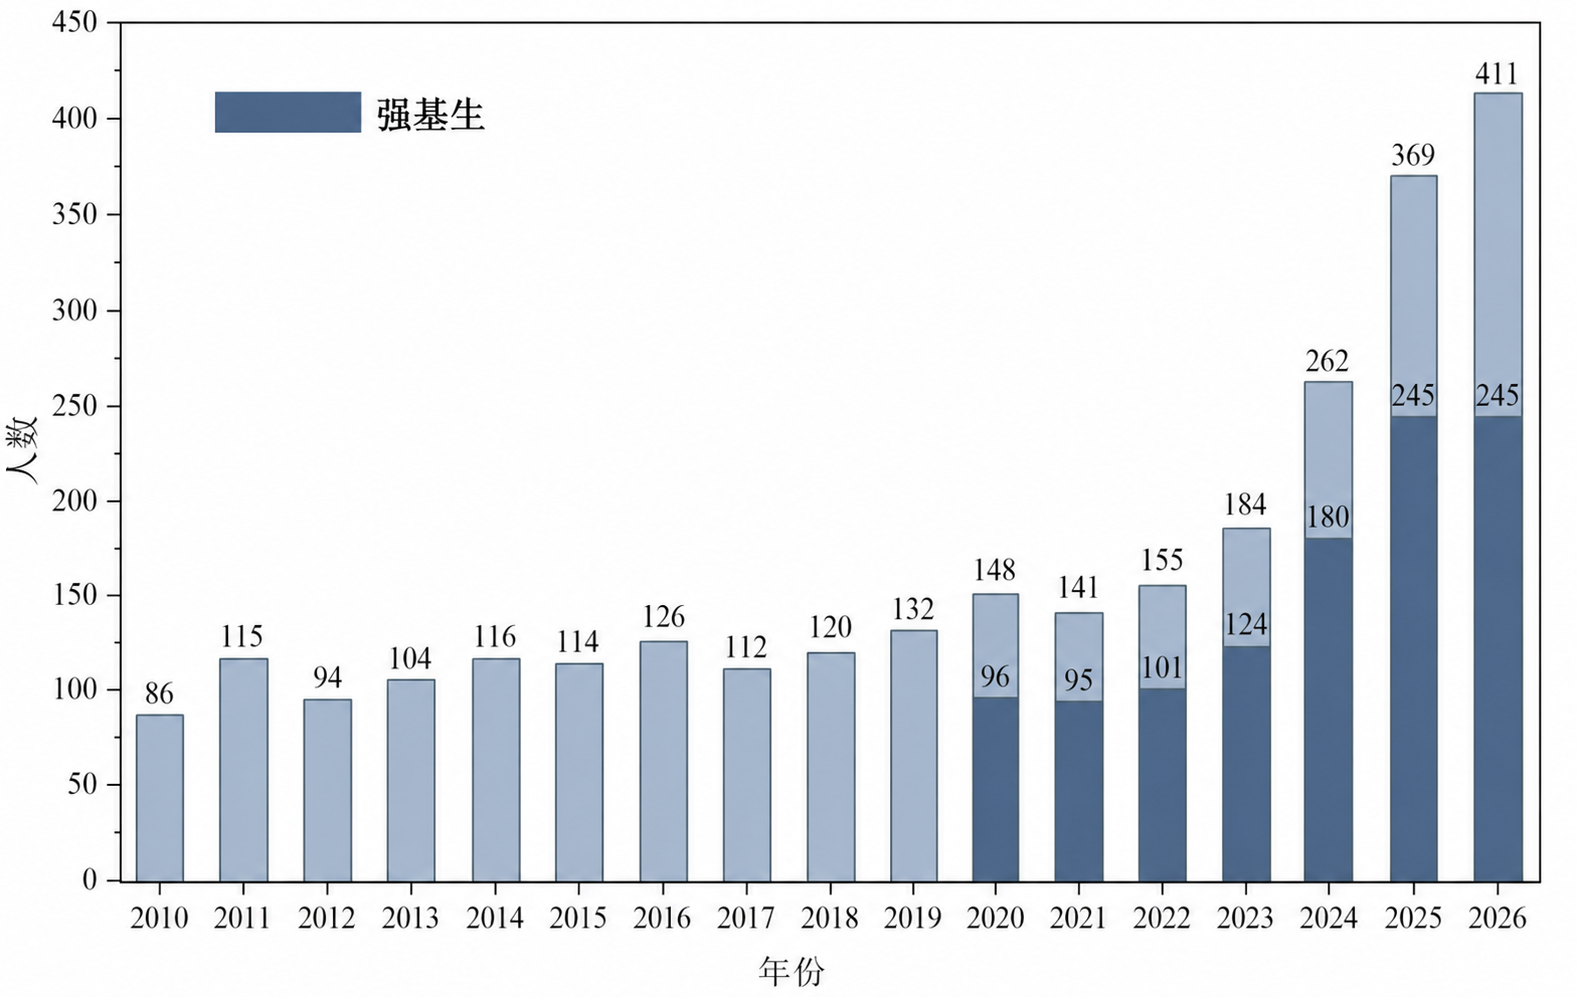
\includegraphics[width=0.7\linewidth]{assets/人数图.png} %需要重新制个图
	\renewcommand{\figurename}{图}
	\caption{工学院近年本科生招生人数}
	\label{fig:enter-label}
\end{figure}

\begin{figure}[H]
	\centering
	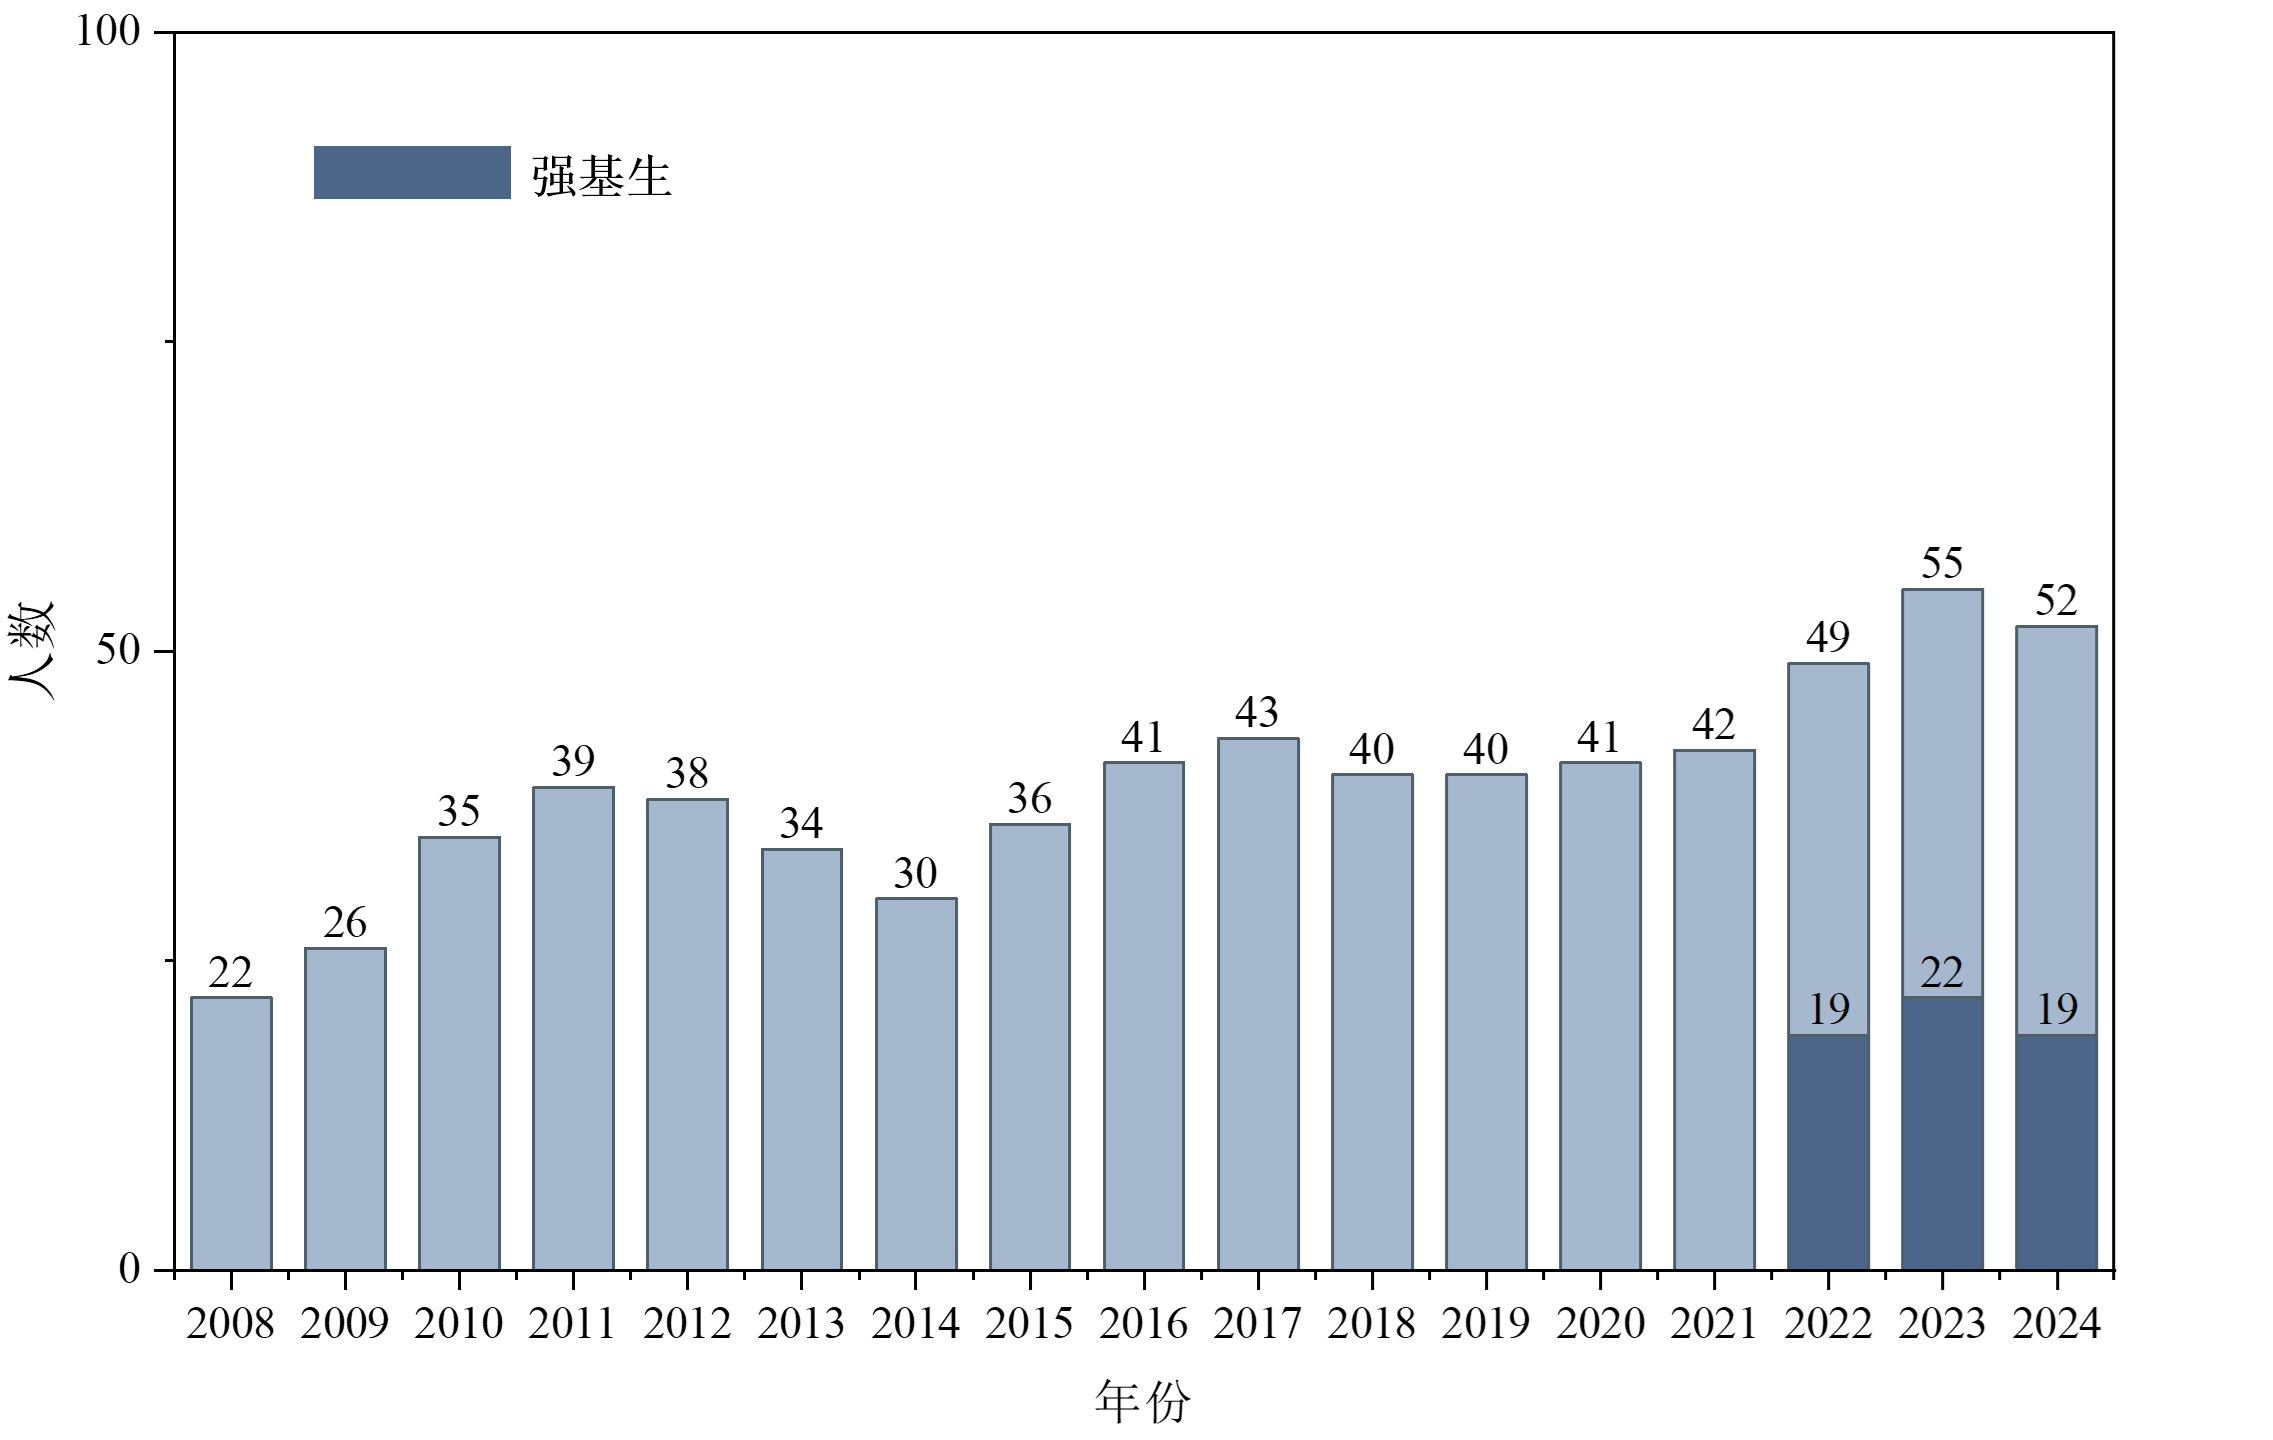
\includegraphics[width=0.7\linewidth]{assets/环科人数图.png} %需要重新制个图
	\renewcommand{\figurename}{图}
	\caption{环境科学学院近年本科生招生人数}
	\label{fig:enter-label}
\end{figure}

可以看出，由于强基专业的增加\footnote{2024年新增化学（材料科学与工程方向）、生物（生物医学工程方向）两专业}、其他院系并入\footnote{2025级环境科学与工程专业本科生的加入}和基础学科扩招，近年来工学院本科生招生人数正在稳步上升。

\vspace{10pt}

大一末分专业方向的时候，每届的同学选择也大不相同。例如：2019级，新设立机器人工程方向，50人左右选择了该方向；2022级选择理论与应用力学方向人数最多；2023级对生物医学工程方向的热情又有所提高；2024级则又对机器人工程方向兴趣较高。每学年末，工学院会召开年级大会说明各专业方向的意向人数，届时同学们可以了解到本年级选择方向的大致趋势。笔者想要指出的是：虽然工学院近年来招生人数不断上升，对同学们的学习生活产生了一定影响，但工学院方向众多，总人数的上升并不一定意味着前路“过于拥挤”，而是可能带来一些新的机遇，例如更充分的学科交流与学科融合。我们希望大家客观评估这一现象。

\subsection{工科试验班与强基计划}
工学院主要从两条轨道录取新生：工科试验班（此类同学后称“工试同学”）和强基计划（此类同学后称“强基同学”）。这两类学生面临的政策有部分差异：

\vspace{10pt}

第一，院系转换。强基计划原始文件中规定：由强基计划录取的学生原则上不能转专业。但在这一点上北大校内政策相对宽容：强基计划专业内部可以互转。工试同学原则上没有转专业限制。

\vspace{10pt}

第二，推荐免试攻读研究生。工试同学走传统的保研路径，强基同学走转段路径。强基同学自带转段名额\footnote{转段名额什么条件下被取消，请自行查找}，而GPA在推免线上的工试同学才能获得推免名额\footnote{针对2024级及之前的同学而言。2026级政策尚不明晰，但也一定和成绩相关，因此大家仍需保证较好成绩}。但无论工试同学或强基同学，推免之后找老师接收这一步，都需要自己进行。在接收方，强基同学存在限制：强基计划有委托培养性质，也就是说，北大的强基生只能保送本校攻读研究生，而工试同学可以找其他院校的老师接收自己。此外，强基计划和工科试验班的同学都不限制考研和出国。

\vspace{10pt}

第三，培养方案。详见教务部官网《北京大学本科教学计划》或工学院官网上的培养方案，其中强基与工试的培养方案会分别列出。

\vspace{10pt}

以上提到的事项（尤其是强基同学）每年具体政策都可能有变化，所以希望大家多多关注相关消息。

\section{细谈本科专业}
以下介绍工学院的七大本科专业方向和环境科学学院的五大本科专业方向，主要采用向高年级学长学姐约稿介绍的形式，内容仅供参考。尤其是与培养方案和修读课程相关的问题，稿件中学长学姐们都以2024级及之前的培养方案作为参考。因此，请同学们在仔细阅读的同时独立思考。不理解或与现行方案有出入之处，还请进一步咨询老师或学长学姐。
\subsection{理论与应用力学}
\subsubsection{（1）2021级\ 谢谊锋}
\textbf{P1 理力专业学习内容}

这里分为四个部分讲解：

\vspace{10pt}

\textbf{第一部分为政治课、英语课、体育课、通识课等课程}，这一部分课程可以有三种心态进行学习：（1）完成毕业学分。北大本科毕业要求学生必须修完这类课程，所以可以选择任务量较少的课程，满足毕业要求。（2）自己感兴趣的方向内容。北大在这些课程的开设上具有很大的广度，所以如果有正好在兴趣点上的课程，可以自由选取。（3）通过这类课程提高成绩。目前对于非强基生而言，保研的推免资格和课程成绩相关。且课程成绩越高，在学年的评奖评优中也有优势。另外，工学院较为重视专业课的学习成绩，所以对于这部分课程，同学们可适当避免那些需要投入过多精力的课，而可以选修一些给分较好的课程\footnote{当然，也会比较难抢上}。

\vspace{10pt}

上述三种心态可能同时存在于一门课程中，这当然是比较理想的情况。但是哪怕不感兴趣，不想在这类课程上花太多心思，也当然是在工院同学中普遍存在的心理，大家不必焦虑。

\vspace{10pt}

\textbf{第二部分为数学、力学、计算机的基础专业课}，下面列举了部分课程：
\begin{itemize}
	\item 数理基础课程：\\数学分析（一）（二）（三）、线性代数与几何、高等代数、常微分方程、数学物理方法（上）（下）、概率论、数理统计……
	\item 力学基础课程：\\理论力学、材料力学、弹性力学、流体力学……
	\item 计算机基础课程：\\计算概论、数据结构与算法\footnote{26级及以后本课程改为人工智能与算法设计}、计算方法……
\end{itemize}

这类课程的具体工程应用性不强，相反，其强调的是理论与概念，对于部分同学来说不是那么直观，甚至是难以理解的。但是希望同学们能够认真地学习这部分专业课，因为这部分知识，对于未来进入到需要数理知识应用的相关场景中时，会有极强的核心竞争力。同时，学院也十分重视这一部分的学习。所以，对于未来希望升学进修的同学，这一部分的学习情况是极为关键的。

\vspace{10pt}

在我的感受中，我是比周围人的理解能力要差一点的人，弄明白一些抽象概念所花的时间比优秀的同学要多一点。但是对于工学院的课程，只要肯下功夫，都是能够弄明白的，所以同学们也需要有自信心。

\vspace{10pt}

\textbf{第三部分为自主选修课}，这类课程同学们可以在全校范围内选课\footnote{注意，部分课程不计入自主选修课学分，详情参见培养方案，或向教务老师确认}。大家可以根据自己的兴趣、科研要求进行更加针对性的学习。

\vspace{10pt}

\textbf{第四部分是工学院的实验课、基础物理课程}。这类课程和工学院专业的关联性较弱，但是实际应用性很强，并且能够锻炼同学们的数理思维，也建议用心学习。

\vspace{10pt}

\textbf{P2 专业未来}

本科就业：

优势很弱，因为同学们花费了大量精力在抽象的数理知识学习上，较为缺乏具体的工程应用经验。并且本人身边的、在理力方向的同学几乎没人抽出精力去企业进行实习。另外，本科学习阶段，同学们的数理基础是比较“泛”的。例如，在固体力学这一块，同学们学到弹性力学便结束了；对于更深层次的塑性力学、断裂力学等课程的知识是没有掌握的。所以，想进入到某一方向的头部就业岗，除了教育培训，其余对口程度都很低。此外，本人也接触过某里、某方等头部企业的研发岗，我认为其工作内容对于我们学习到的这些抽象数理概念利用率低，而工作重心是在满足甲方要求的前提下，用最低的成本和最简洁明了的、最安全稳定的、最高效速成的方法完成甲方要求的项目。当然，北大文凭还是很强的敲门砖，并且同学们的学习能力也很强——这是我们的优势区间。

\vspace{10pt}

升学科研：

这是工学院大部分同学的选择，同学们通过在工学院本科阶段的学习，正如我前面提到学习的科目是很“泛”的，所以同学们是很可能找到和自己兴趣、能力相匹配的科研方向的。并且在这一阶段，可以将之前学习到的数理知识这一“内功”练就为一门独特的“外功”，将核心竞争力培养得更加具体化。

\vspace{10pt}

\textbf{P3 学习体会}

成熟的培养方案：

得益于力学系的悠久历史，本培养方案中的数理课程甚至是北大很多任教老师上过的课程，也是很多优秀毕业学长学姐们上过的。因此，经过时间长河的检验，这一培养方案在培养数理基础认知上是极为成熟的。同时，这一培养方案与具体内容也是不断革新的，保证了同学们可以在掌握基础的同时，对于力学相关前沿问题也能够有更加全面的认知和更为广阔的视野。

\vspace{10pt}

学习过程是十分辛苦的：

无论是本科生还是研究生阶段，力学系的学习都是需要同学们花费大量时间和精力的。相比其他方向的同学，力学系的卷度是更高的。力学系同学若希望取得较好成绩、专业排名，则需花费极大的精力。即使是像我这样大多数数理课程在优秀以上、自己擅长的数理课程能拿90+的同学，也是极为刻苦的。并且，以我对头部同学的观察，他们更加用功。

\vspace{10pt}

对力学数理知识有敬畏之心、好奇之心，并以在其中探索为乐，同学们的付出是可以得到回报的：

包括我在内的大部分同学，都认为我们在数理基础知识学习上投入的时间精力是得到了具有极强幸福感的回报了的。具体内容的确因人而异，所以这一部分我不具体展开描述，就留给同学们自己去发现吧。

\subsubsection{（2）2021级\ 杨铮昊}

传统的力学专业分流体和固体两派。我们最早会在大二下学期接触到的材料力学，就是固体力学的范畴，而直到大三我们才会通过两门必修课——流体力学（上）、流体力学（下）——入门流体力学这门学科。我挺建议对固体力学不是很感冒的同学，提前了解一下流体力学的内容，或许你就能更早发现自己的兴趣其实在流体。除了这两派以外，工院的力学与工程科学系还包括了许多其他的力学分支，如生物力学、力学系统与控制，也包括如流固耦合等一些交叉学科。这些方向需要学习的内容都不会出现在培养方案的推荐课程内，所以建议想要探索的同学尽早去联系对应的老师，寻求指导和帮助。

\vspace{10pt}

理力专业的课程方面恰如其名，围绕着“理论”与“应用”两个主题。在低年级优先学习的数学课和力学课都是为了打下扎实的“理论”基础，而大二下学期的材料力学实验，才正式开启“应用”的实践。如果学习理论课程时没有那么得心应手，不妨多去尝试一些实验课。这里的“实验”并不仅限于实验室里的实验，也包括那些需要动手编程的数值模拟实验。因为在未来的科研中，真实实验和数值实验都是推动科研的重要手段。

\vspace{10pt}

理力专业的课程难度总是被排在第一，因为比其他专业多出一些“更难”的数学课。但对于大多数专业而言，要想行稳致远都离不开扎实的数理基础，而理力专业只是更多强调了这一点且体现在了课程设置上。所以无论是选择哪个专业，基础数学课都一定要认真学习，力求扎实掌握。

\vspace{10pt}

有玩笑说各行各业都有理力专业的学生，这其实不假。通过本科阶段的学习，理力专业的学生应该有信心收获较为扎实的数理基础和动手能力。今后无论是在哪个领域从事科研或是就业，二者都能提供强大的竞争力。另一方面，如果你能够尽早地确定未来的奋斗方向、尽快入门并启动，更是一件好事。所以本科阶段除了沉淀和积累，很重要的一点就是多向外探索。

\vspace{10pt}

作为在此专业学习已达三年之久的“老登”，我还是感觉很幸福的，因为无论是老师还是同学都特别友善包容，让我既能在良好的学习氛围中收获满满，又敢于做出许多探索和尝试。但如果这个专业不适合你，同样放心寻求老师的帮助就好。

\subsubsection{（3）周培源班}

周培源书院（或周培源班，后简称周班）是工学院理论与应用力学专业方向专门开设的一个小班。有关招生政策基本信息，请有意向的同学多多关注学院官网报名通知，也可通过12月学院举办的工学嘉年华、大一下学期举办的若干次选专业指导讲座进行了解。

\vspace{10pt}

以下是周班的学长给大家作的补充介绍：

\textbf{周班介绍\quad 2021级 钱骏飞}

\vspace{10pt}

\textbf{\textbf{一、发起周班的动机及培养目标：}}

秉承“培本固源，笃行秀出”的理念，旨在培养出具有深厚数理基础和人文素养、追求长远科学目标、能够引领力学学科及未来新技术创新发展的杰出人才。

\vspace{10pt}

\textbf{\textbf{二、周班与普通班培养的差别：}}

目前周班同学接受的培养方案和普通班是完全一致的。在课程上的差别是，周班同学接受的是小班化教学，授课内容会略多于平行班，课程的考核难度也会较高。考虑到周班的同学们都很优秀，课程都是不限优秀率的。不过客观来说，给分并不是很香。如果大家希望的是更好地打牢自己的数理基础，多和身边优秀的老师同学们交流，同时对分数不是特别care，则非常建议大家来周班进行学习。但如果之后有出国的意愿，或者对分数看得比较重的话，一定要慎重选择，在周班想取得特别高的分数肯定是要比普通班难好多的。

\vspace{10pt}

除此之外，周班的一大优势就是灵活。每隔一段时间\footnote{大约是一学期一次左右吧}，周班的主管老师们会和同学们进行交流，询问一下同学们目前的学习情况，以及对课程进度的一些看法。如果建议得当的话，很有可能会进行一定的课程改革，比如将某些课提前一学期进行学习，或缩短/增长学时。在选课方面，周班可以进行课程替代。例如，国家精品课基础物理实验，就可以通过选修数院的实变或微分几何来替代。原则上说，必须要选取难度更高的课才能进行替代。至于具体到哪门课可以用哪门课来替代的话，最好要向周班主管老师荣起国老师询问确认好，并且经过教务老师同意。整个流程操作起来虽然略显复杂，但是真的很有用！

\vspace{10pt}

学习之余，活动也是不少滴！周班会为大家尽可能地安排讲座、报告等活动，带领同学们充分了解科技前沿进展，帮助大家认清未来可能从事的科研方向。假期会不定期组织同学们出国参观，并进行学术等各方面的交流，例如之前五一去了马德里和巴黎，暑假去德国等等。综上所述，课余生活还是很舒服的！

\vspace{10pt}

进入周班的门槛并不高。只要大家数理基础别太烂\footnote{会有个面试，别被老师拷打得太狼狈一般就没问题}，愿意接受这种培养方式，几乎就能成为周班大家庭的一员。

\vspace{10pt}

\textbf{\textbf{三、周班的转入转出机制}}

对普通班的同学，想在周班选拔之后进入周班也是可以的。你需要提前与周班的主管老师们联系好，征得同意后达到一定条件即可转入。周班的同学们倘若迫于课业压力而想转去平行班的话也是可以的，与老师们提前沟通好就行。

\vspace{10pt}

值得注意的一点是，普通班的同学可以选修周班的小班课来替代普通班的课，但周班的同学不可以修普通班的专业课来替代周班的专业课。一旦如此操作，便会被视为退出周班。

\subsection{工程与科学计算}
\subsubsection{（1）2021级\ 吴秉宪}

在我的理解中，工算方向的教学目标是培养一批兼具数学、力学基础和计算机编程能力的同学，初衷是为工业软件的设计和工程领域的计算任务积累后备力量。因此，工算的培养方案同时包括了数学分析、线性代数、高等代数、常微分方程等数学基础课，理论力学、材料力学等力学基础课，计算流体力学、计算固体力学等结合了计算背景的力学课，以及一系列与程序设计或优化方法有关的课程。

\vspace{10pt}

下面我仅站在个人立场分享我在工算方向学习三年以来的一些心得。

\vspace{10pt}

工算课程所涉及的范围较广，且很多课程之间关系不大，例如并行程序设计、计算机图形学、工程CAD、机器学习基础等。每门课基本都是一门全新的学问。这一点容易让人感到矛盾。一方面，我们能在本科阶段接触到计算机在不同子领域的应用，对完全不同的技术都有所涉猎，便于探索自己感兴趣的方向；另一方面，课程的广度不可避免地造成深度的欠缺，每门课可能只能帮助我们窥见一角，想要深入挖掘还是需要自己在课外花额外的时间。而且课程的广度意味着培养方案前后衔接得不十分紧密，每门课想学好都得花足够的时间。对于我来说，培养方案中的肯定是存在屑课的\footnote{这就需要灵活运用课程测评来避雷了，樂}。但我并不介意这样的培养模式——本科期间能够多尝试一些方向是一件好事。

\vspace{10pt}

那么，什么样的同学适合选工算？我们当时分流时，除了理力方向占绝对优势外，最受欢迎的应该就是工算了。我想，这可能是因为那时计算机热潮仍然占据主流。随着现在新能源、生医工、新材料的需求和热度升高，近两年几个小方向的人数几乎都差不多了。我认为在这样的趋势下选专业时，自己的生涯规划是最重要的。对于有明确目标或者兴趣要去某个行业的，就不必再看接下来的建议，只管在契合的领域大胆冲就是了。因为工学院不同方向之间的差异很大，本科就提前接触自己感兴趣的方向肯定更好，也更容易寻求升学的机会。对于没有明确兴趣的同学，我想从培养方案的角度给一些建议。如上所述，工算的培养方案会包括很多和计算机相关的课程。这些课虽不像信科的专业课那么硬核，不会涉及底层的架构设计，但是往往还是需要写一些代码的。所以很排斥写代码的同学也许不是那么适合这个方向\footnote{虽然现在似乎不管什么方向都需要会写一些代码了，悲；但现在可以用AI写代码了，乐}。大家可以通过大一的两门公共计算机基础课程感受自己对写代码的接受程度。工算的课程比较广比较杂，所以单论数理基础，肯定不如理力方向打得扎实，课程难度也相对低于理力。如果对于力学强烈感兴趣，或者对知识体系有很高的要求，建议去理力方向\footnote{当然，这个要求是其他所有方向都满足不了的，不只是工算。工算大概已经是理力之外对数理能力要求最高的方向了}。不过反过来，对于像我这样对力学没太大兴趣、想要尽可能规避力学课程、同时又比较喜欢程序设计的同学，工算就是一个很不错的去处。一些有志转码但是大一的时候还没下定决心转专业的同学也可以选工算作为一个跳板。

\vspace{10pt}

最后，关于工算方向未来能做的事情，我想说，事在人为。我觉得工算的同学在数学、力学和编程上都能够打下良好的基础。课程太杂的弊端常会让我苦恼本科好像没有系统地学到什么，无法直接将课堂所学应用于实践当中。但是不可否认的是，在遇到一些需要学新东西的场景时，这种通才的本领能够帮助我们比较快地上手。以保研为例，工算的同学可以回头继续研究力学\footnote{其中工程力学系应该是和工算方向直接对口的}，可以去对数学和编程有较高要求的工管系、控制系和机器人系，也可以去信科的几个研究生院寻求机会，甚至可以找一些与本专业无关但是恰好需要会做计算的同学参与研究的实验室。总体而言，工算的选择还是非常多的，重要的是敢不敢去尝试。保研的这几种途径里，大多数都需要主动地联系导师争取机会，尤其是跨院系保研。很多同学包括我自己都对自己的能力不够自信或者觉得专业背景不够契合而畏手畏脚，但是也有一些同学去尝试了就获得了offer。希望大家可以趁还有时间多去尝试，定好目标大胆去冲，我相信我们专业的出路基本都是挺好的。
\subsubsection{（2）2022级\ 曹林博}

我将从专业感悟、课程内容和学习心得三方面为大家介绍。

\vspace{10pt}

首先，从专业研究内容来说，工算需要通过计算机解决工程中的问题，比如设计、优化、仿真预测等问题。这里我引用袁子峰老师\footnote{力学与工程科学系助理教授}的观点：“我们在解决工程问题时，利用仿真方法得到的数值结果是对客观现象的近似描述，而这个过程是多个层面的问题。”我们需要经过理论公式的推导，构建合适的数学和力学模型来描述解决的问题中折射的客观现象（通常是偏微分方程体系），其次需要通过设计与证明（如稳定性、收敛性、鲁棒性）来生成一个可行性好的算法，最后通过代码编程实现这个算法。当然，工算专业课程的广泛性与紧凑性，也为我们研究其他领域内容提供了可能：代码能力的培养让我们将人工智能融入研究内容中，数学物理思维的锻炼让我们也能够投身传统力学的研究，甚至解决超越力学的物理过程的科学计算问题。因此，我们可以在本科生阶段（主要是前三年）通过旁听导师组会、与学长学姐交流、与老师面对面交谈、参访实验室等方式，探索自己的研究兴趣点，以为研究生阶段做准备。

\vspace{10pt}

其次，从课程体系上说，根据我们的研究内容，我们需要上数学类、力学类、计算机类三大类课程。

\vspace{10pt}

力学专业是非数学专业里面用数学用得最勤的，对数学的应用可以达到“润物细无声”的地步，因此我们需要夯实数学基础，这也为以后对于工程问题的符号化表述和逻辑性解决提供数学基础。工学院的数学课程比如常微分方程、工程数学、数学分析系列、高等代数等，需要将老师的讲义、PPT、参考教材结合起来，达到相互补充、帮助理解的作用。

\vspace{10pt}

力学类课程是我们工学院的看家本领，是我们区别于纯IT人员的重要特质。掌握力学的知识体系，才能为我们设计算法提供科学基础。理论力学、材料力学、流体力学等力学课程，需要我们通过习题的训练，将力学的知识应用在具体问题中，从而提高对力学知识的掌握。

\vspace{10pt}

计算机类课程培养我们使用计算机的能力，旨在将计算机作为一种工具，从而帮助我们实现模型的建立和问题的优化。计算概论、数据结构与算法会让大家学到编程语言最基础的语法和数据结构，计算几何、计算机图形学、并行程序设计等课程会在提高编程能力的同时，拓宽大家的视野，亲身体会到计算机是如何为科学研究发挥作用的，初步了解工业计算软件的代码编写规范，为我们提供了解科研和投入科研的机会。

\vspace{10pt}

最后，从我两年的学习心得出发，想对我大一时候存在的疑惑进行解答，这些问题可能大家初入工院的时候都会遇到。首先大家需要摆脱高中时候凭他律学习的学习方式，大学里的时间和精力是自己自由分配的，因此需要大家对自己的学习情况和生活情况做到心中有数，学会把握自己的生活节奏。其次大家需要多与老师和学长学姐交流，放下羞涩。老师和学长学姐们都是非常热心和善良的，乐于帮助大家解决问题，这也有利于培养大家与他人相处的能力。最后大家要对自己有信心，相信自己，追求热爱！

\vspace{10pt}

祝大家能够在北京大学工学院这个大集体中，熠熠生辉，光芒万丈！

\subsection{能源与环境系统工程}
\subsubsection{（1）2022级\ 付杨}

工学院能源专业\footnote{包括力学类强基能源方向，以下统称能源专业}的培养单位是力学与工程科学学院能源与资源工程系（以下简称能源系）。能源系成立于2005年，与重建工学院同年，是院内历史最久的系之一，不过在院内的存在感不算太高\footnote{这是能说的吗×}。

专业内容上，北大能源专业和工科院校的能动专业有不小差异，这和北大工科与传统工科的差异是一致的。考虑到能源技术更新迭代快，我们减少了不少具体的工艺或工程技术类课程\footnote{当然在工程热力学等课程中仍能有宏观了解}，同时增加了底层通用的理论基础课的比例。简单说，北大能源专业的核心是“热”，因此我们有三门从不同角度切入的热力学课程——工程热力学、物理化学、热力学与统计力学导论，还有传热传质学、热质传输数值模拟、渗流物理等课程介绍热量和物质的输运；能源系统分析与优化、新能源技术、化工原理等则从不同视角展现能源系统及相关领域。当然，还有大量数理基础课和力学基础课为专业课学习筑牢根基。对强基同学来说，会多一些像材料力学B这样的理力专业课程；相应地，非强基同学的必修课，能源与环境工程实验，会变为选修课，但整体课程体系差别不大。

\vspace{10pt}

学习体验方面，作为强基生，我同时修习过力学系和能源系的课程，能明显感受到两系在授课习惯、考题风格上的差异。能源专业涉及的力学系课程\footnote{如线代、概统等数学课，理力、工流、材力等力学课}历史悠久、体系成熟、范式完整，老师授课风格和高中阶段较为相似。期中/期末考题也比较规范，且因选课人数多，大多有往年题可参考，备考时大致能把握方向，老师也不会大幅调分。所以建议大家稳扎稳打，尽量吃透每道作业题。能源系的专业课，课堂听课感受可能不像力学系课程那样“条理清晰/体系完整”，考题也更灵活，对知识融会贯通的要求更高。但好在系里老师给分都比较宽松，只要认真学，都能有不错的收获\footnote{但过程可能会比较痛苦}。

\vspace{10pt}

有两门课想特别提一下：能源与环境工程导论，本科生实践大课堂。能源与环境工程导论（简称“能环导”）是大二的第一门专业课，前半学期介绍环境污染、环境监测等环境相关内容，后半学期每周会邀请一位能源系老师介绍自己的研究方向（例如碳封存、油气资源开发、能源政策、热管理等）。这门课既能让大家对能源专业的研究范畴有整体认识，也能为后续选择课题组提供参考。本科生实践大课堂是能源系独有的本科生科研形式。和一般的本研/短期本研不同，它不以出成果为目标，试错成本很低——哪怕一学期下来没得到像样的成果（前提是确实用心投入了），也是被允许的。通过一年的探索，大家能初步明确自己的科研兴趣，还能培养基础的科研规范和技能。

\vspace{10pt}

总之，能源系在工学院是规模较小的系，老师和学生人数都不多，所以基本都能互相认识，日常氛围轻松，偶尔还会组织春游/秋游、午餐会等活动。欢迎对能源与环境领域感兴趣的同学加入我们～

\subsubsection{（2）一位希望保持匿名的同学}
\textbf{一、专业情况概述}

\begin{figure}[htbp]
	\centering
	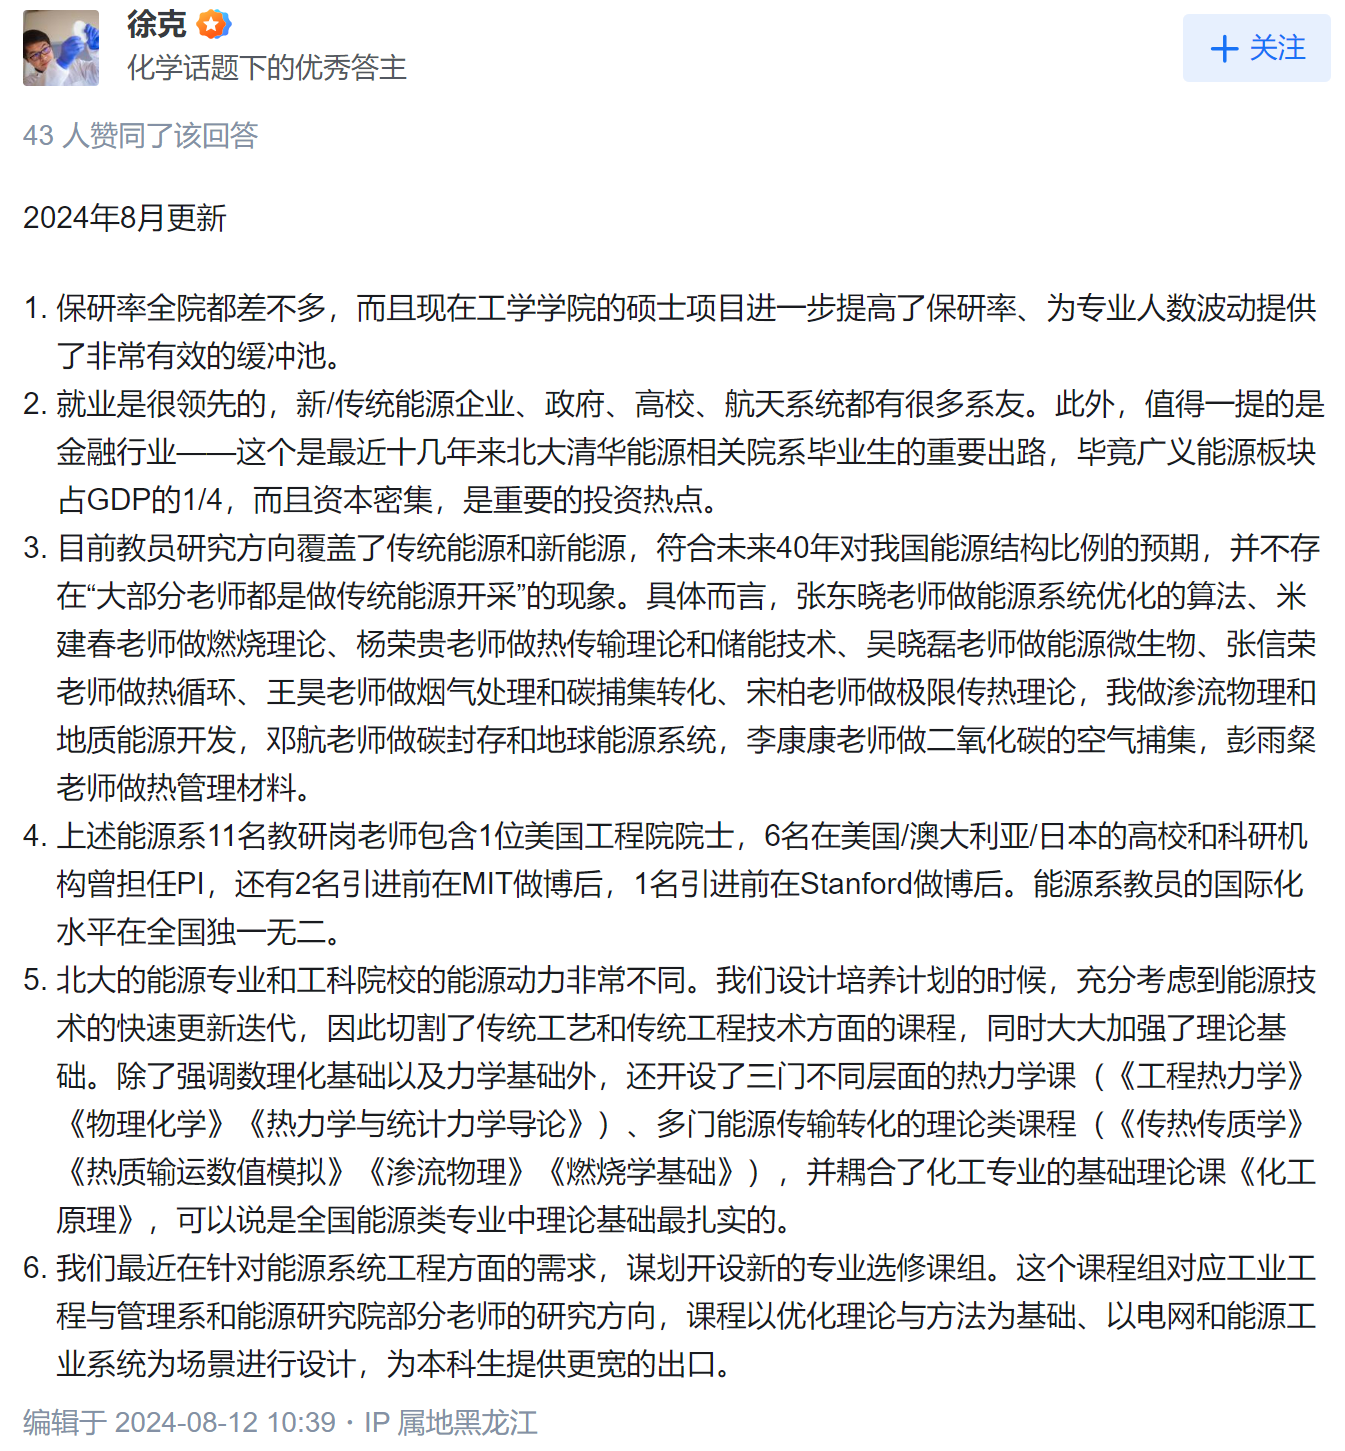
\includegraphics[width=0.7\linewidth]{assets/1.3.3徐克老师问答.png}
	\renewcommand{\figurename}{图}
	\caption{徐克老师知乎回答}
	\label{fig:enter-label}
\end{figure}

转自能源系徐克老师知乎回答。恰如陈正老师在树洞5G冲浪一样，能源系的徐克老师活跃在知乎一线。徐克老师对保研、就业、老师科研方向、课程设置等都进行了较为详细的讲述，同学们可以重点关注第3点。

来源：https://www.zhihu.com/question/583497117

\vspace{10pt}

\textbf{二、能源专业学习内容}

1. 非工学院（体育、通识、政治、英语）课程。

对于能源系的同学们来说，由于本专业课程难度相较理力等专业课程难度低，同学们可以有更多时间学习感兴趣的通识类课程。建议提前在树洞、课程测评等网站善用搜索，尽量不要选择给分迷惑、投入大于回报的课程即可。

\vspace{10pt}

2. 基础必修课

\begin{itemize}
	\item 数理基础课程：数学分析一、二(非强基同学可用高等数学B上下替换)、线性代数与几何、概率与数理统计、普通物理ⅠⅡ、普通化学B、（常微分方程）、（工程数学）……
	
	\item 力学类课程：工程流体力学、（理论力学B）、（材料力学B）、……
	
	\item 计算机基础课程：计算概论、数据结构与算法、计算方法……
	
\end{itemize}

括号标注的课程对于工科试验班（非强基）的同学是建议的自主选修课程，对于强基的同学是专业核心课（必修）。

\vspace{10pt}

大部分基础课程都会在前三个学期完成，对于能源专业来说，在培养方案上减少了部分数学课程，部分课程难度相较理力等专业降低，如用工程流体力学替换了流体力学。因为强基同学必须以理论力学为主修专业，所以理力专业部分核心课程仍是必不可少的。

\vspace{10pt}

这里需要注意的是开设在大一下学期的普通化学B和高等代数两门课程。由于在第二学期结束时才会选择专业方向，而部分专业要求必修普化B，部分专业要求必修高代，可能会需要在大二、大三之后补选相关课程。对于确定选择能源专业的同学来说，在大一时可以选择不修难度较大的高等代数。

\vspace{10pt}

虽然常微分方程、工程数学不是能源专业同学必修课，但在后续的学习中，相关课程知识还是会被用到。比如在工程流体力学中就会涉及求解常微分方程、以及工程数学中的复函数等。

\vspace{10pt}

3. 专业核心课
\begin{itemize}
	\item 热力学课程：工程热力学、传热传质学、热统导论……
	
	\item 能源传输转化类：传热传质学、热质输运模拟……
	
\end{itemize}


能源系专业课相对难度较低，易于理解，大多是基于热学、力学之上的课程，部分涉及化学中的热力学内容，如吉布斯自由能、熵、焓等相关概念。请大家相信有努力就会有回报。

\vspace{10pt}

4. 能源专业特色课程

这部分主要列举一些个人认为能源系在培养方案中比较有独特性的专业课。

\begin{itemize}
	\item 能源与环境系统工程导论（能环导）。这门课是能源专业大二上学期开设的专业基础课程，类似于工学院在大一上学期开设的现代工学通论。2023年秋季由邓航老师开设。课程前半学期主要由邓航老师讲解环境保护与修复、后半学期由能源系多个老师以讲座的形式讲解能源和资源的开发、生产、应用，老师大多会结合自己目前研究的方向课题进行介绍，是了解老师，选择自己感兴趣方向的机会。
	
	\item 金工实习。这门课程是由材料学院开设于暑期的能源专业必修课程。会安排去昌平校区住5天左右，住宿环境很好，课程给分很好，涉及车床加工、3D打印等多项具体的加工技术操作，是一门很好的工程生产实践体验课。
	
	\item 本科生实践大课堂。这门课是能源系面向大三年级开设的科研实践类课程，可以说是能源系自己的本研\footnote{指本科生科研。本手册后续内容对此有进一步介绍}。在第一节课会有多位老师介绍自己的项目供同学们选择，除了能源系自己的老师外，还有工管、先机、材料专业做与能源方向有关的老师。学期中主要跟随相应老师进行科研实践，期末以答辩汇报的形式完成。
	
\end{itemize}

\textbf{三、专业未来}

大部分同学主要的选择都是升学科研。能源系提供了很好的本科生科研环境，有利于同学们在本科阶段找到自己希望在研究生阶段继续学习研究的方向。此外，能源系大部分老师都有海外科研背景，国际化水平高，对于希望申请出国留学的同学来说，也有一定的帮助。

\vspace{10pt}

\textbf{四、学习体会}

1. 培养方案注重理论基础，学习过程注重工程实践。

能源专业是一门工程类专业。但在工学院整体注重数理基础、能源技术更新速度快的影响下，北大能源系的培养方案切割了传统的工程技术、更加注重理论类课程，而工程实践类的技能则是在鼓励同学们参与到老师的科研课题中学习的。

\vspace{10pt}

2. 以兴趣为导向的自我探索，非常nice的师生氛围。

能源专业课内学习相对不卷，但可能随着专业人数逐渐增加有所变化，同学们可以将更多精力放在本科生科研上或其他自己更感兴趣的领域。能源系经常组织一些师生聚餐、学长学姐本研升学经验分享等交流活动，帮助大家多次、详细地了解老师们的研究课题，找到自己感兴趣的方向。除此之外，每学期还会有班主任、辅导员交流聊天环节、期末考试学生宿舍走访慰问等等，及时解决同学们学习生活中的困难。

\subsection{航空航天工程}
\subsubsection{（1）2021级\ 柴宇澳}

北大航空系主要以理论研究为主，注重理论基础，可以算是力学专业的延伸。近年来航空系不断发展壮大，主要体现在：陈正老师转入航空系；连续多位教师入职；学生选择人数上升。主要的研究方向有：燃烧与航空发动机设计、流体力学、气动声学、一般力学等。航空系一些基础课程与理力要求相同（如高等动力学、材料力学等），增添一些航空航天相关课程（空气动力学、航空航天概论等），也会较理力少一些理论课（如固体力学等）。总而言之，难度比理力较低，但是内容很多都与理力（尤其是流体力学）相关。

\vspace{10pt}

航空航天工程系前景广阔，一是在航空航天科研院所工作（航天三院、五院、九所......很多很多）；二是在国企、私企工作（大疆（无人机相关）、华为（燃烧与电池相关）、美的（流动控制与湍流相关）等）；三是出国深造，后续在高校任职。

\vspace{10pt}

从我个人的学习体会来看，航空系的课业压力比理力小一些，相比于其他专业也不卷。航空系有许多优秀又有趣的老师：在空气动力学课上，吕本帅老师送给我了一架飞机模型，吕老师还带我们去参观航空航天博物馆；在航空航天工业实习课程上，周超老师带我们去密云放飞航模与无人机。陈正、黄迅、刘才山、李存标、程承旗、史一蓬等老师都是在各个领域登峰造极的教授。同时，在保研方面，航空系的老师更加愿意接受来自北大的本科生，航空系的保研率也因此非常高。不过航空系出国这方面可能会有签证上的困难\footnote{针对美国高校而言}，需要仔细衡量。个人感觉在航空系就读体验良好，氛围融洽，同学们相互学习，也不会盲目攀比内卷，就业选择也相对较多，适合对航空航天、流体力学等有兴趣的同学选择。

\subsubsection{（2）2022级\ 鞠志翔}

航空航天工程是和理论与应用力学比较相似的一个方向，在本科培养上削减了一些理论性较强的课程，如高等代数、弹性力学、数学分析三，以及将一些课程压缩学时偏重应用来讲，如数学物理方法上下压缩为工程数学，流体力学上下以工程流体力学替代等等。此外，有一些航空航天特色的课程，主要是工程热力学、飞行器设计与动力、飞行器结构力学、空气动力学基础。在升学上，既可以考虑航空航天的导师，也可以考虑理力的导师，如果是后者建议多学习（不一定选课）一些理力的课程，以应对夏令营的面试。

\vspace{10pt}

在航空航天工程专业本科培养方案中，除去计算机基础课、通选课、体育课、思政课、英语课等全校必修课程以及自主选修课程，专业课主要分为基础专业课、专业核心课和专业选修课三类。其中，基础专业课包括数学分析、线性代数与几何、普通物理。专业核心课为材料力学（及实验）、理论力学、高等动力学、飞行器结构力学、工程流体力学这种力学课，以及工程热力学、飞行器设计与动力两门主要涉及热力学的课，还有一门电子电路课和工程性较强但难度不大的空气动力学基础。专业选修课中有三门是必修的数学课，它们是常微分方程、工程数学和概率与数理统计；其他课程按照学分要求选课即可，其中计算方法、控制理论基础（自动控制原理）是相对用处较大的；工程制图个人感觉对后续学习基本没有帮助且任务量大；普通化学(B)和普通物理类似讲的杂但容易刷分，但对后续学习帮助也不大；航空航天工业实习非常水，可凑学分。

\vspace{10pt}

建议学弟学妹除去培养方案上的专业课，适当选修或旁听一些课程，比如数学分析三、高等代数、信号与系统等可以填补知识漏洞的课，举例来说，航空航天工程的培养方案只有数学分析一与二，缺乏级数的学习，此外工程数学也不会细讲傅立叶变换，而信号与系统会详细讲解。

\vspace{10pt}

下面根据几门个人选过以及印象较深刻的课程，向同学们分享一些具体课程的心得体会，希望可以帮助大家提升学习体验，其中基础专业课在此略过，线性代数与几何、普通物理一二以及常微分方程的笔记放置于北大网盘（见文末）中，可供同学们参考。此外，查看树洞中的课程测评也会给大家带来一些收获。

\vspace{10pt}

（1）电子与电路\ 黄迅老师 

评分机制：30实验 + 30开卷期中 + 40开卷期末

作业不计分。按照原始总分的排名给分，100到85一名次一分，85以下会有调整，给分很好。

\vspace{10pt}

上课建议认真听，中文掺杂英文，老师考点都会在课上说；课本是英文，考试可以带。课本建议按要求看完弄懂，其实干货不多。期中很靠后，基本是期末的预演。期末大部分会考期中原题，考完期中建议和同学把答案对出来。不建议考前突击。实验课为在面包板连接电路，并下载一些电路模拟软件，扣分不多。

\vspace{10pt}

（2）工程热力学\ 张信荣老师

评分机制：20作业 + 30大作业设计 + 50期末

如果不想选航系开的工程热力学，张信荣老师的课是个不错的选择。这门课课堂听感一般，会点名但不要求考勤，因此适合考前突击。期中设计超临界流体火箭发动机，认真写报告即可。期末偏重概念的考查，填空和简答占大部分，老师课上会讲一些例题计算题，期末大概率会考计算原题，给分很好。

\vspace{10pt}

（3）空气动力学基础 吕本帅老师
评分机制：25期中 + 35期末 + 40平时分，包括一个大作业

\vspace{10pt}

这门课程很多知识在工程流体力学和工程热力学中已经学习过，比如等熵流动、不可压无旋平面流动复势这些知识。新增加了一些结论性的知识，绝大部分计算都可通过查表代替公式计算，因此可以期末前突击记结论。

\vspace{10pt}

最后感谢观看，在本科学习过程中的一些学习资料已经放在网盘：

https://disk.pku.edu.cn/link/AA1EA6B17FBAC44A65AAF79260DB132729
中，大家可以参考。最后祝各位学弟学妹在燕园学业顺利，生活愉快！

\subsection{生物医学工程}
\subsubsection{（1）2022级\ 范文琳}

生物医学工程是一个所含内容非常广泛的专业，几乎任何涉及生物或医学问题的工程类实践都可以被划进这个范畴。因此，相比于具体知识的传授，生医系的专业课更加注重项目式的学习，并且会对一些科研和工作上的“软”技能有一定的侧重，比如小组合作、presentation、文书撰写等。生医系比较有特色的课程是系列PBL课程（i.e.生物医学工程原理、生物医学工程设计）。在这些课程中，老师会要求同学们以小组为单位，在一个学期内完成一个课题的文献研究，或实现一个小型项目。过程中同学们可以向任何可以得到的资源寻求帮助，主管课程的李长辉老师也会为各组提供一些如何求助的指导与建议。

\vspace{10pt}

科研方面，生医系对于本科生提早进行科研实践给予极大的鼓励。生物医学工程专业对口的老师很多，但具体的研究方向之间也相去甚远，包括成像、计算、电子，也有偏向纯生物的课题组。大家可以在未来技术学院官网上查看老师们的研究方向，通过和老师约谈或者听组会的方式来决定自己更加感兴趣的方向。一般而言，大家会在确定自己的方向之后在选课上进行一些调整，以规避交叉学科学习中通常存在的“博而不精”的问题。

\vspace{10pt}

另外值得注意的是，尽管生医系的强基生被要求修一系列力学系课程，但这些课程在难度要求上和正统的力学系课程还是有一定的区分。当然，任何理工类学科中数理基础总是重要的，诸君可以自己多多留意（x）。

\subsubsection{（2）2022级\ 李昆泰}
\textbf{生物医学工程系概况：}

生物医学工程系（常简称生医系，后文亦沿用，这个名字可能小有误导性，之后会在文章中详述）和材料系是工学院“系”、“专业”或“方向”中较为特别的两个，因为实际上生医系和材料系的“研究生院”都是单独成院的，它们对应的学院分别是未来技术学院和材料学院。未来技术学院这个学院可能在大家看来相当“科幻”，觉得我们搞的好像是什么天顶星科技一样。在某种意义上确实，我个人也觉得我们在创造一些极为有意义的工程发明和科学发现。更实际地说，北大的未来技术学院面向的就是未来的生命健康，所以也无怪乎生物医学工程系是在未来技术学院中的一个系了。简单理解的话，生医系是未来技术学院的一个系，而这个系的本科生放在了工学院这个学院中进行培养。大家如果选择国内深造，大概率可能会选择进入到未来技术学院的课题组中。

\vspace{10pt}

\textbf{生医系的入学渠道和同学构成：}

生物医学工程系现在应该有三个入学渠道。一是高考裸分录取中的“工科试验班”类，二是强基计划力学类的“理论与应用力学（生物医学工程方向）”，三是强基计划生物类的“生物四”。其实在大一选专业后，实际进入生医系就读时没什么差别（生物IV我现在不清楚），编班都在生医班，成绩排名、评奖评优什么的都在一起排，也享有同等的进实验室等的资源。差别主要在培养方案上：强基需要比非强基的同学多修一些力学类课程，数学类课程的难度要求可能也会高一些；非强基的同学则需要修读更多学分的生医工专业相关的课程。

\vspace{10pt}

\textbf{生医系在做什么：}

前文说了，生医系是未来技术学院的一个系；同时，生医系还是未来技术学院唯一的一个系。大家未来路径选择上很大的一个优势就是——本科从生医系毕业，研究生可以选择整个未来技术学院的方向\footnote{当然也可以选择如生科、人工智能等其它学院的方向，这里讨论的是主流的选择}。所以，与其说是在讨论生医系在做什么，其实更多讨论的是未来技术学院整体在做什么，乃至整个生物—医学—工程领域的交叉点上大家在做什么。

\vspace{10pt}

先从“狭义”的生医系本身讲起。这里要澄清一个长久以来的误解：生医生医，其实是生医工这个“生物医学工程”的简称的简称，“生”和“医”是工作面向的核心问题和应用场景，“工”则是这个专业的“技能”核心。大家可能会认为生医系是做生物科学研究的？还是当医生的？进检验科的？等等等等，其实都不甚准确，或者说不是标准的路径。准确地说，生医系可以说是给生物科学研究造更好的仪器设备，让科学家看得更清楚，操作得更“稳准狠”，打开更多的研究可能性的工作；是给医生创造更好的医疗器械和临床工具，或者给患者本身制造更好的健康检测、干预与辅助设备，增进病人的生存率和福祉，为更多疾病带来创新型的治疗与干预方法的工作。它的学科基础主要是工程学和物理、化学、生物学；关注的是解决生物科研和医疗临床问题\footnote{北大生医系前者做的较多，但社会上主要谈的是后者}；而在未来，它更有可能带来大幅长寿、人机融合等人类社会的重大变革。

\vspace{10pt}

在临床领域，生医工所做的可以看到的工作已经非常丰富了。大到CT、磁共振、超声等各种医疗器械，小到血压计、血糖仪、血氧仪等日用医疗健康产品，再到嵌入到智能手表里的心率检测等功能，都是生医系（与其他学科交叉融合）的创造。脂质体药物、CAR-T等创新疗法其实也可以称之为一种“针对生物的面向医学需求的工程学”，所以这个学科有相当的学科交叉性和知识结构多样性。进一步的，在“广义”的生物-医学-工程领域上说，我们会在各个尺度、各个物理原理上进行创新。我们会利用力、热、光、电、声等物理原理，酶促反应动力学等化学原理和激素调节等生物学原理，一方面探测生物从分子细胞到个体群体的各种信息，另一方面用这些自然的力量去扰动、调节乃至控制生物系统，以增进对生物系统的理解和对人类调控生物系统的手段的掌握；另一方面，我们会从物理的疆域跨越到信息的疆域，利用算法、大数据与人工智能的力量对我们获得的信息与能力进行更强大的总结、提炼与应用。这些抽象的理念具体化到各种方向中，就是生物成像\footnote{利用光学获取细胞及亚细胞尺度的信息}、生物力学\footnote{工学院可能做的比较多，提取生物学现象中所蕴含或利用的力学规律}、神经电生理和神经工程\footnote{通过电信号收集生物体的信息和对生物体进行扰动或控制}、生物传感器与生物电子学\footnote{利用电子元器件构建对不同物理信息的提取装置}、生物探针\footnote{利用蛋白质等生物分子的相互作用原理与光学等物理原理实现对生物系统的观测}等等。

\vspace{10pt}

未来技术学院还有分子医学所、国家生物医学成像科学中心、大数据与医学人工智能系等机构，其研究方向其实也在我刚刚讨论的广义生物—医学—工程交叉领域之中。相关的研究方向和实验室也是大家可以去尝试、选择的。在真正的科研实践当中，尤其是生物—医学—工程这个大的领域之中，科学与工程、发现与发明、研究与创造、提炼与综合一直是相互交织、相生相荣的关系。我们很难划出一个到底什么是生物科研，什么是生物医学工程，什么是分子医学研究的分界。但只要大家对生物学问题、医学问题和针对二者的工程问题中的其中一点有所兴趣，都欢迎大家来到生物医学工程这个广大而充满无限可能的领域中探索与创造。

\subsubsection{（3）2022级\ 丁奕航}

生医工专业近几年的变动比较大。作为22级的本科老登，我的分享主要基于自己力学强基的身份，兼有对非强基培养方案的一定了解。对于26级生物强基的同学，可能只在部分方面有参考意义（叠个甲先）。

\vspace{10pt}

生医工专业是一个非常广泛的专业。广义地说，任何在生物或医学方面的工程相关课题都属于生医工专业。北大的生医工内部也分为多个方向，主要包括分子细胞、成像、生物计算、生物材料等，每个方向都各有特色。由于强交叉的学科特性，往往每个方向所需要的专业能力都是多样而不同的。因此，建议同学们从大一开始就多多了解各个方向的具体情况，大致包括这个方向在做什么事、有哪些老师在研究哪些具体项目、可能需要哪些知识技能、自己是否感兴趣等。这一过程不必着急，通过专业课的学习、与老师同学们的交流、校内的各种讲座课程和官网上的教授主页等慢慢熟悉即可，主要是为了明确自己的兴趣方向。

\vspace{10pt}

生医工专业本科期间的学习和科研是紧密结合的。由于专业内各个方向区别较大，培养方案内的课程难以深入每个方向，更多是普遍地教授一些初级技能，给同学们一个初步认识。因此，大家往往需要在明确一个兴趣方向后尽早地进入老师的课题组，通过读论文、跟项目等方式，在应用中学习具体的实验操作、软件使用和更为细致的生物医学和数理力学知识，将其与课内学习相结合。这样的模式一方面需要大家一定的自学能力，另一方面可能也需要大家权衡课内外学习，放弃一部分课的优绩，换得更实用的技能。关于学习部分，还想多劝大家不要过分重视绩点，在专业人数持续增长的过程中不要被焦虑裹挟去卷一些没必要的事，而是为自己找到适合的方向，由兴趣和实用需求驱动，放松心态去锻炼一些自己需要的能力。即便是从功利角度出发，在保研和留学中绩点也并非第一指标，只是一个够用即可的门槛。学习能力、科研经历、乃至于合作能力、人际交往能力和性格等软性特点才是老师们更看重的。

\vspace{10pt}

在生医专业的学习中，还需要注意根据不同学科课程的特性调整自己的学习方式和习惯。我们的培养方案要涉及数理化生医等多种课程，其中数理（力学）课更注重理解推理，而化生医学课往往需要更多的记忆。用适合一种课程的习惯去学另一种课可能会吃亏，一定要注意避坑。（说来都是辛酸泪）

\vspace{10pt}

关于保研，第一当然是及早联系老师，在大三暑假前尽量有一点点实在的科研经历。这主要是因为夏令营时科研经历是最主要的考察项目，老师可能会问一些较为深入的问题，科研水不水一问便知。第二是建议多方面了解，不要仅限于未院，校内叉院、生科乃至信科等院系的一些项目都可以尝试，非强基的同学也可以联系外校老师们\footnote{如果政策没有变化的话}。第三是不要太在意沉没成本，当你觉得自己和当下的课题组不合适，直接换就好，毕竟直博是五年的相处，比很多恋爱都长，还不能轻易分。关于出国本人不甚了解，不过在本科低年级需要做的事相差不大，在此就不赘述。

\vspace{10pt}

最后，祝愿大家在工院快速扩张内卷加剧的当下，还能始终保持初入燕园的这种兴奋、好奇与探索欲，在这多彩的校园和有趣的专业里，享受短暂而美好的大学时光。

\subsubsection{（4）一位希望保持匿名的同学}

个人主要参与以实验为主的方向，且非强基，所以力学课学得比较少，以下讨论都基于这个前提展开（首先叠甲）。

\vspace{10pt}

\textbf{关于方向：}

我了解的实验室大多与生科方向较为接近，但整体而言更偏向临床应用，个人认为在科研中属于比较容易找到获得感与方向感的方向。实际参与过程中的主要感受是，这类动手较多的实验，仅仅在课本上学习或是在网上看视频，和自己亲自去参与一个完整的实验流程所感受到的是非常不同的，想了解相关方向的话也许可以早点去实验室了解一下，而且上手做过后也会更容易理解相关论文的研究方法等。

\vspace{10pt}

\textbf{关于上课：}

由于本人是高数B + 医预有机B选手，这两年的深刻教训就是基础课需要亿点练习，和分子细胞、生理学这样“会背=会做”的课不太一样，这些基础课的考试由于题目不少+难度不算特别高+不调分，所以几乎每一分都是要靠平时的努力和汗水自己做出来的（悲），仅仅理解完全不练习可能直接导致在交卷前对着会做但来不及写的题目发出尖锐的爆鸣，不过相信小灯们带着刚从高中训练出来的新鲜大脑，还是能轻松应对的（确信）。

\vspace{10pt}

最后夹带一些私货，推荐几个也许不是必修但有意思的课程\footnote{“有趣”的评价出于个人喜好，可能对一些未来倾向不同研究方向的同学来说比较无聊，另外尽管开课老师都非常nice但没有水课}。

\vspace{10pt}

（1）sky\footnote{即“生科院”的首字母}杨竞老师的免疫学。个人觉得老师讲课很有意思！虽然受限于课时很多细节没办法在课程中全部覆盖到，但作为入门了解感觉很不错；

\vspace{10pt}

（2）孙红芳老师的生物医学工程综合实验。我以前没学过生物竞赛，在该课程中可以学习到科研常用的实验操作及原理，并且练习一项很重要的技能——自己看protocol学习新实验的操作；

\vspace{10pt}

（3）胡薇薇等老师开设的文献写作与报告。虽然是通识课，但正如胡老师在开课时所说，这门课或许在通识课里有一点“硬”，但能坚持下来的同学一定收获满满，个人认为能经过几周甚至一两个月的准备，精读一篇论文，从其研究背景到方法、结论，流畅地作一次模拟学术汇报，可以对自己感兴趣的研究方向有更深入的了解并且锻炼一下学工科后日渐贫瘠的表达能力，很有成就感（还弥补了本人组会第一次讲journal时磕磕巴巴的遗憾hhh），并且听听其他不同专业同学的汇报，还是挺有意思的。

\subsection{材料科学与工程}
\subsubsection{（1）2021级\ 李一川}
材料专业学习的知识会涉及更多的领域，包括物理、化学、生物等多个方面的知识，课程内容也比较丰富。同时，在注重基础知识学习之上，会更加强调与实际应用和生产生活相结合。课程讲述的内容也非常前沿，许多也是当前社会发展的热点话题，比如钙钛矿半导体、新能源电池、柔性电子等等。材料学院目前已经单独成立学院，导师数量众多，涵盖的研究范围也非常的广，对接资源非常丰富，同学们可以根据自己的兴趣，非常自由的选择导师加入课题组进行本科生科研训练。

\vspace{10pt}

材料专业的本科教育更加强调基础知识的学习，以及大量细分领域的了解，拓宽知识面，而大部分同学会选择在本科毕业后继续在某一个专业领域继续深造，攻读硕士或博士。

\subsubsection{（2）2022级\ 曾帅鹏程}
\textbf{关于基础课程：}

1. 全校通选：全校学生情况都差不多，但作为工院学生尤其会对三四类通识感兴趣，所以务必注意一二类通识选择时一定要选核心通识课，避免多修。

\vspace{10pt}

2. 工院基础：以数分、高代等专业课程为代表，在大一未分流时，全体学生情况统一（强基与非强基会略有不同，具体请研究培养方案）。值得注意的是，工学院对数理的要求较其他理科学院来说有过之而无不及，且范围广（计算机、数学、物理、化学都有涵盖），务必对此多加上心。若对材料专业感兴趣，建议大一下修完大学化学，减少之后学期负担。

\vspace{10pt}

3. 材料专选：在大一后分流来到材料专业，需要修习许多专业课程，强基生不能完全丢掉理论力学的学习，因此课程任务量会比大一学年加重。理论力学方向相关课程会和生医、能源一起开班上课，难度略低但也不可轻率。材料方向课程则以小班授课形式进行，代表课程有：材料科学基础、材料物理、物理化学、材料学中的量子与统计……这些课程理论性极强，会结合当前材料方向前沿进行讲解，内容在化学基础比化院较弱的情况下会显得晦涩难懂，但很有必要花费大力气进行深度学习。工学院的课程课后花费时间一直位于北大第一，希望同学们早做心理准备，但也要相信，只要肯下功夫，成绩也不会辜负你的努力。

\vspace{10pt}

4. 自主选修：这方面课程需要和你的研究方向相结合，材料学的知识十分广博，在确定好自己今后学习方向后特异性极大，结合方向多修习校内相关课程，方能使学业一帆风顺。

\vspace{10pt}

\textbf{专业未来：}

材料学本科就业不占优势\footnote{其实除去金融和计算机，很少有专业会愿意本科后就业}，在读完研后\footnote{听说本校通常给博}就业方向极广。材料学科囊括范围极多，从本校导师研究方向便可管中窥豹：肿瘤疫苗、电催化、锂电池、纤维、钙钛矿、高分子等。所以需要尽早确定从事材料科研的方向，毕竟任何一个方向都需要精深学习，都需要花费时间。在研究生毕业后有许多出路：博后发展、企业研发、高校任职、科研所任职等。具体内容都是因人而异。

\vspace{10pt}

\textbf{学习体会：}

在化学基础较化院薄弱的情况下，每一门材料的课程都会显得晦涩难懂，每一门专业课程都需要在课后投入大量时间进行学习。但要相信，每一分努力都会带来回报。材料专业对科学前沿的了解十分重要，所以了解自己方向的科学前沿发展情形都很有必要，需要自己课后花费时间进行了解。

\subsubsection{（3）2023级\ 惠炜博}

\textbf{关于课程学习}

材料专业与其他传统力学类专业很大的区别是，在分流之后的第一年就会将学习范围极度拓宽，数学、物理、化学和更加交叉的方向都有所涉及，我本人是工科试验班类（非强基），对这种变化的体会尤为深刻。当然这也意味着在选择材料专业之后有了一次重塑的机会：课程不那么依赖大一数理课的基础，继续付出努力仍然有可能在材料专业闪闪发光。

\vspace{10pt}

由于工学院本科生的化学基础较弱（此处是对非化学强基的同学而言），在上材料专业的核心课如：材料科学基础、材料物理、材料中的量子统计的同时，还需要在普通化学B的基础上学习物理化学、有机化学B、分析化学等课程，相当于是边打地基边造楼。尤其是物理化学中有很多重要的基础内容，却被放在大二下学期。不过各位也不必过分担心，与化院相比，我们所学的基础化学类课程已经是减学分、减学时、减内容之后的版本了。只要肯认真学习，还是能够满足考核要求和基本的知识体系构建需求的。此外，由于排课学期和排课顺序等因素，负责教授专业核心课的老师们可能会选择在自己所讲的部分向大家补充前置知识。在这里也建议各位想选择材料专业的同学们要培养充分的自主学习能力。

\vspace{10pt}

材料专业的课程（基础化学类课程除外）目前来说基本形成了一种范式，即课堂讲授＋小组文献汇报＋习题课（若有平时作业）＋闭卷考试，考查的能力也是多方面的。关于小组文献汇报，老师会给出一些和课程内容有关联的文献，同学们自己去选择自己感兴趣的文献进行研究和汇报，一般来说时间在20至25分钟。有的老师比较排斥对着稿子读或者是当PPT reader，所以这个部分需要很强的表达能力和变通能力。关于习题课，即老师或助教将具体的题目分配给具体的同学在特定的一节课来讲解自己的思考和解答过程，几乎没有选择空间，讲题的过程也非常考验表达。关于闭卷考试，材料专业核心课需要记忆的内容偏多（非常多），理解的东西也不少，比较考验记忆力和知识体系化的能力。

\vspace{10pt}

\textbf{关于就读体验}

尽管自己觉得不算轻松，但不得不承认，与工学院其他专业相比，材料专业的课程难度总体上较小。只要肯付出努力，稳扎稳打，基本都会取得比较不错的结果。此外，大部分老师会在上课时向同学们介绍自己的实验室所研究的课题方向，也很愿意跟同学们进行课间交流，让大家在官网之外能够有更加生动的了解。如果是像我一样的工科试验班同学，在大二时就可以免于上很多3学分4学时的课，留出更多的学习时间去做其他事情，例如了解老师、旁听组会、进实验室做本研等。外界（甚至我们自己）经常调侃“生化环材”是四大“天坑”，但其实翻看材料专业老师们的主页就会发现，他们从事的大部分都是迎合新时代国家发展战略需求的研究。大部分材料专业的同学会选择本科结束之后再读研究生，而在材料专业的保研压力也相比其他专业要小很多。

\subsection{机器人工程}
\subsubsection{（1）2021级\ 刘家豪}
\textbf{专业内容}

从本专业的必修课设置看，机器人系统的设计、制造中所涉及的各环节内容均有覆盖，课程涵盖集成电路、控制器、机械设计、建模等内容。个人认为通过本科阶段的学习，了解制作完整的机器人所需知识，掌握MATLAB、SolidWorks等常用软件的使用，甚至自己DIY一些简单的机器人应不成问题。在专业必修课的主线之外，亦有较为丰富的选修课程可供体验，譬如机器学习、嵌入式、图论、计算机视觉等相关课程。

\vspace{10pt}

总体来看，作为一个多学科交叉的本科专业，机器人工程的课程设置更注重广度，培养能力全面的人才。建议结合本科课程的学习、实验课体验、本研经历选择自己感兴趣的具体研究方向。如果对机器人领域感兴趣的话，相信本专业能够给你良好的学习体验。

\vspace{10pt}

\textbf{自身体会}

就我个人三年来的学习体验而言，与其他工科院校的类似专业相比，本专业也较为注重数理基础的培养，这也是本校工学院的院系特色之一，具体体现为大一需要完成多门基础数学课的学习，后续也有较多数学类课程可供选择。学有余力的同学可以尝试本院的“理力+机器人”双主修项目。

\vspace{10pt}

若要达到精通某一具体的机器人领域，以作为将来科研或就业道路的立身之本，我认为仅完成本科阶段的课程学习可能并不足够，课外的自学和实践也很重要。本科学习期间适当参与科研项目或竞赛更有助于自身技能的完善，如大二下学期报名参与自己感兴趣的本科生科研项目等。

\vspace{10pt}

\textbf{未来去向}

若想继续从事机器人领域，相比与直接本科就业，我个人认为读研深造可能是更为合适的选择。下面我就我个人的了解大致介绍与本专业相关度较高的科研方向。由于本专业涵盖较多学科的内容，相关可供选择的科研方向亦丰富多样，在此仅举一些我较熟悉的例子。例如从事某一细分领域的研究，以机器人感知为例，硬件如视觉、触觉传感器等的设计，软件如多传感器融合算法、SLAM等，都是可选的方向；又如完整机器人系统的设计，譬如特定用途的机器人如某一类医用机器人、水下机器人、软体机器人等；将AI与机器人融合也是时下较为热门的方向。另外，进入工学院官网浏览本系老师的研究方向或咨询学长学姐等，或许能让你对本专业的科研方向有一个较为全面的认知。

\vspace{10pt}

我个人对于本科就业了解不多，在此也就不过多介绍。进入相关科研院所工作、加入科技公司或某些大厂的机器人研发部门，一般是较为对口的选择。当然，有了北大计算机通识课、专业相关课程所积累的编程基础，进入互联网企业工作也不失为一个选择。倾向于就业的同学可以多多留意院系宣讲时介绍的毕业去向统计或咨询学工办老师。

\subsubsection{（2）一位希望保持匿名的同学}
机器人工程专业涉及多个领域的基础课程，包括力学（理论力学、高等动力学）、数学（高等代数、常微分方程）、电路（如数电、模电）、机械（如机械设计基础、机器人学概论）、自动控制原理等。这些课程是入门的基本要求，也是未来深入学习和研究应用更具体内容的基础，需要大家都能有一定程度的掌握。因此，对于想要选择机器人专业的同学来说，前两年的首要任务就是重视这些基础课程的学习。

\vspace{10pt}

除了基础课程的学习，第二个关键任务是主动探索本专业的研究方向。机器人专业涵盖了多个研究方向，包括智能系统与控制、群体博弈与智能决策、医用机器人、水下机器人与装备、先进制造与工业软件、无人系统的自主决策与规划等\footnote{大家可以到工学院官网查看更具体的内容}。建议大家积极利用各种机会，如现代工学通论课程、各类讲座，以及与老师的交流，去更加深入地了解每个方向的研究内容。在还没有明确的兴趣时，多与老师交流将大有裨益。在对各个研究方向有了一定了解后，就可以选择一个合适的时机，主动联系老师，参与一些本研任务。最初可能有忐忑和顾虑，但是这种边学边用的学习模式，给予我们很大的成长进步的空间，不仅能够加深对知识的理解，还能提升解决实际问题的能力，最重要的是也能检验我们是否真正感兴趣\footnote{如果发现自己实在不感兴趣，那么就去探索下一个方向，试错空间很大的！}，这对我们的自身发展能起到更全面的帮助。

\vspace{10pt}

此外，在后续的课程学习和本研中，MATLAB、Python以及SolidWorks等软件将会频繁使用。因此，建议大家提前自主学习+练习这些工具的基本操作内容\footnote{迟早都需要自学的}。

\vspace{10pt}

希望大家在选专业这方面上不会有太多的困惑啦，如果有，那就及时主动寻求帮助！愿大家能够享受这段美好的时光！

\subsubsection{（3）2022级\ 欧阳卓}
\textbf{专业学习：}

在专业必修课中，首先最基础也是最重要的是一些数学物理和力学的课程，俗话说“像科学家一样思考问题，像工程师一样解决问题”，这些基础课程可以让你对基本的理论体系有一个初步的了解，搭建起自己脑中的“科学大厦”。进一步是关于机器人相关的专业课程，以我的理解可以大致分为三层：

\vspace{10pt}

底层设计：

对于机器人，底层的机械结构是机器人的骨架，我们可以通过例如机械设计基础、先进制造基础等课程了解机械结构设计的方法、机械的加工制造等方面的知识，并学习诸如工程 CAD、SolidWorks 等软件的使用方法；

\vspace{10pt}

“血肉”铸造：

电子电路、单片机、传感器相关电子元件好比机器人的血肉，它们将底层机械结构有机地结合起来，使得机械臂能动起来、机器人能像人一样“看见”外部信息，通过模电、数电、机器人学实验二等课程可以对电子相关内容有个大致的了解；

\vspace{10pt}

“大脑”控制：

对于机器人来说，顶层的算法、规划、控制等内容就像机器人的大脑，当机器人通过传感器得到相关指令后，大脑会对这些指令进行处理，并告诉机器人下一步该怎么做、怎么将信号转换为动作并实现。这一部分涉及内容较广，可以通过一些计算机算法相关的课程和控制等相关课程来学习。

\vspace{10pt}

上述三部分内容仅仅是我的个人见解。以我个人而言，我会通过专业必修和选修课对各个部分进行一个初步的了解，然后会对自己感兴趣的方向进行更广泛、更深入的了解。比如我对机械不是很感兴趣，但会继续选一些微电子、机器学习、强化学习的课程，对电子和算法层面有更多了解。

\vspace{10pt}

\textbf{科研方向：}
机器人可选择的科研方向很广。你可以尝试机械的项目，进行一些机器人实物的设计；也可以进行嵌入式开发、对电子电路进行深入的探索；同样也可以进行优化控制的研究。进组也会拥有更多元的选择。我在大二时，就是先加入了智能学院王弈森老师组进行机器学习的研究。大二下也旁听过机器人系李忠奎老师组，大三上加入了工管系尤鹏程老师组进行强化学习、优化控制等方向的研究。大家在选择科研方向的时候思路可以打开，不一定仅仅只局限在自己的专业领域，因为你会发现开始科研时很多知识你都得从头开始学，所以不要因为这个领域你不熟悉就气馁，更不要觉得自己专业对口就能很轻松地解决科研问题。

\vspace{10pt}

\textbf{个人体验：}
关于自身学习体验，这里我主要谈谈课内选课、学习等方面。

\vspace{10pt}

1. 关于选课，前面很多学长也谈到了，在这里我还想说一点我关于绩点\footnote{考虑到从2025级开始取消绩点制度，请大家将其看作是“成绩”的同义词}的认识。成绩的高低有很大一部分来自选课的规划，比如你选了一门好课，可能你比别人花更少的时间就能拿到更不错的分数。这样说可能有点功利，但对于较为看重成绩的同学来说，选课是你同样要花很多时间去规划的一件事，因为选择有时候比努力更重要。

\vspace{10pt}

2. 有的新同学可能会有很多东西想学，一学期一不小心就选了一大堆专业课和通选，想要挑战自己。以我的经验和个人见解，这样一来，可能会因为课业压力过大而心态爆炸，导致过早实现绩点自由\footnote{指绩点处于较低水平，产生“无所谓”的态度}（一学期八门十门专业课还能3.9+ 的大佬除外）。另外，很可能因为课程过多，你会把大量时间花在写作业、做lab和应付考试上。一学期学下来成绩不错，但回过头来发现很多东西只是浅尝辄止，并未深挖，学过了就忘了。第三，从我个人角度，上课并不是学习效率最高的方式，如果你有足够的自律（这个前提很重要！），你完全可以只学基本必修课，其他想学的课程都自行找资料学习，这样可以省去很多无用的作业、无用的内卷以及考前背诵一些犄角旮旯的东西的时间。但说实话，我觉得上课会通过作业、考试、绩点等方式逼迫你学习。如果没有课程的压力，自己又没有足够的动力（无论是热爱还是单纯的自律），时间可能就都用在摸鱼划水玩游戏上去了。最终知识没学会，学分也没混到（本人的惨痛经历 ×），故这一点因人而异。

\subsubsection{（4）2023级\ 石昊}

\textbf{专业理解：}

正如培养方案第一句话所说：“机器人工程专业是……涉及机械、电子、力学、计算机、自动控制、人工智能等众多学科。”工学院的机器人工程是一个涵盖学科非常多、学习内容非常广的专业。就拿课程设计来说，本科阶段需要修读的课程涵盖了机械、电子电路、力学和计算机等方面。同时，该专业也对学生技能的广度和深度提出了要求，包括但不限于计算机编程、SolidWorks建模、Arduino控制和PCB电路设计等。个人认为工学院机器人工程专业的课程设计比较合理，其涵盖了机器人领域最底层的知识体系和技能点。不过，鉴于专业的特性，不可避免地会因为学习的内容太多太杂而导致学生对日后的方向产生迷茫和焦虑。而且，不可否认的是，相较其他工科类院校学习机器人的同学，贵校\footnote{指北京大学。“贵校”是北大同学口中对北京大学的调侃称呼}机器人工程专业的同学在动手做项目或者做科研方面的经历会比较少。理论固然重要，但是作为一个工科学科，实践经验要比理论学习更重要。这个时候可能需要同学发挥主观能动性，积极寻找科研和项目的机会，比如联系导师进课题组和参加有关的机器人比赛等。

\vspace{10pt}

\textbf{就读体验：}

就我个人来说，在机器人专业的就读体验是很不错的，主要有以下几点。首先，正如前面所说，学院设置的课程体系全面涵盖了机器人领域的核心知识。同时，得益于北大自由的选课制度，如果对计算机、AI和电子这方面的知识有更深的需求的话，还可以选择信科的课程来完善自己的知识结构，也为个性化发展提供了广阔的空间。此外，机器人工程专业拥有开放包容的学术氛围。以我的切身体会为例，我经常和同专业同学及课题组成员展开深入交流，既探讨课程内容，也分享研究思路。这种思维的碰撞，不仅拓宽了我的专业视野，更显著提升了我的学习效率和科研创新能力。此外，作为工学院2019年设立的新兴学科，机器人系汇聚了一批十分优秀的青年教师。他们的加入为专业发展注入了强劲动力，使整个学科呈现出蓬勃发展的态势。这也让我个人觉得机器人系正生机勃勃，蒸蒸日上。

\vspace{10pt}

\textbf{给学弟学妹的话：}

我在前面也说到了，由于需要学习的内容太多太杂，很多同学可能会迷失方向，产生焦虑和不安的情绪。我认为尽早联系导师进组是个明智的选择。即便暂时不直接参与具体研究，单纯观察前沿科研人员的工作状态和研究内容也极具价值——正所谓“他山之石，可以攻玉”。学习和借鉴他人的创新成果，往往能帮助我们逐步沉淀出自己的研究方向。同时，在学习和科研过程中，积极与同学和老师交流往往会有意想不到的收获。我个人也正在寻找未来的方向，上面的话也谈不上建议，更多的是和学弟学妹们共勉。学弟学妹们刚步入大学校园，可能会感到焦虑和不适应。其实本科的试错成本是很低的，大家可以勇敢尝试自己感兴趣的一切事物。无论遇到什么困难，希望大家保持乐观，坚信一切都会越来越好。不管同学们之后是否会选择机器人专业，祝愿大家一切顺利，都能够找到自己喜欢的方向，日后能在自己的领域里发光发热！

\subsection{环境科学与工程}

\vspace{10pt}

\textbf{环境化学}


\subsubsection{（1）2022级\ 王成昊}

环境科学与工程学院主要包括四个专业方向：环境科学、环境工程、环境健康与环境管理。通过强基计划进入北大的同学修读的是环境化学专业，在后续研究生阶段才需要从以上四个方向中选择一个自己感兴趣的方向。环院老师的研究方向十分多元化，从大气物理、大气化学，到仪器开发、材料合成，再到生态学、微生物学，以及经济学、管理学、法学和伦理学都有涉及。具体的专业情况和老师研究方向，可以到学院官网的“师资力量”一栏查阅。需要额外指出的一点是，环境科学与环境工程这两个方向研究内容实际上有着一定的交叉与重叠，具体选择时更应关注导师的具体方向，不必拘泥于某一专业方向。在选择本研导师或者研究生阶段导师时，可以广泛地搜集老师们的资料，尤其是最近发表的文章，了解老师们目前感兴趣的方向。此外，也可主动约老师聊天或旁听组会，感受课题组氛围与工作重点。

\vspace{10pt}

环境学科作为一个问题导向性学科，其最终目的在于解决实际问题，因此课程设计上会比较“宽口径”。环境化学专业的课程大致分为三大模块：一是夯实数理基础的公共必修课，包括高等数学、线性代数、概率统计、计算概论等；二是建立化学根基的化学类必修与选修课，其中不少课程与化院专业课直接对接；三是旨在掌握环境专业知识的环境类必修与选修课。由于课程涉及范围较广，教学内容跨度较大，想要每门课程都追求完美不太现实，建议结合自身实际情况和未来发展方向综合考虑，合理分配投入到不同课程上的精力和时间。

\vspace{10pt}

关于选课，还有几点碎碎念。首先，切勿仅凭课程名字臆断课程内容。选课前最好看一下课程的教学大纲与安排，同时搜集一下这门课的往年评价，确认其确实符合自己的选课需求后再选课。其次，不必畏惧中期退课。如果在课程学习中压力过大，且期中成绩十分不理想，在确认后续有机会重新选课后，最好不要硬撑，果断退课，保住成绩方为上策。最后，需要强调自学能力的重要性。不同课程的授课风格不同，如果课程教学方法和进度不适合自己的节奏，一定程度上选择自学或许是一个不错的想法。此外，大学的学习也不必拘泥于课堂，本科生科研、学生工作、社会实践、社团活动、课外时间也都是学习的机会。

\vspace{10pt}

环境作为一门相对冷门的专业，每届都会转出不少同学，继续留在本院的同学大多会选择继续深造，也有少数选择直接就业。对于是否转专业这一问题，我认为转专业是非常正常而且合理的选择。但是转专业的前提是对转出和转入的专业有着比较充分的了解，同时有着较为明确的职业规划。专业各有利弊，找到既喜欢又适合的方向，是大学阶段最重要的一课。

\vspace{10pt}

最后，真诚欢迎各位同学加入环院大家庭！祝愿大家能够在大学四年间，感受大学的酸甜苦辣，寻得自己真正的热爱与理想，度过一段“五味俱全”的充实生活。

\subsubsection{（2）2022级\ 陶安然}

\textbf{（1）学习内容}

我们的专业课主要由环境科学与工程学院和化学与分子工程学院两个学院开设（以下简称“环院”和“化院”）。其中化院开设的课程主要有普通化学、定量分析化学、有机化学、物理化学和一些实验课程。相比于化院的学生，我们学习的化学课程难度低一些，对于有化学竞赛基础的同学来说，化学课程的学习是比较轻松的；没有化学竞赛基础的同学则要做好啃硬骨头的准备，但是认真学习也是可以学懂并且获得不错成绩的。环院开设的课程主要有环境问题、环境科学、环境监测、环境工程（一）（二）等，和非强基专业学生的基础环境课程比较一致。当然了，计算机基础课和基本的数学课也是我们要修读的，鉴于之前的部分数学课对同学们来说难度较大，学院对培养方案中的数学内容做了调整，希望大家能拥有一个良好的数学学习体验。

\vspace{10pt}

\textbf{（2）个人学习体会和建议}

环境化学的学习内容还是很有趣的。我觉得与其他专业较为不同的是，我们能将学习到的化学相关基础知识应用到具体环境问题上，从分子结构出发解释环境现象的机理。本人没有化学竞赛的基础，所以在刚刚入学时，学习普通化学这门课要付出比较大的时间精力。但根据身边统计学，是否有竞赛经历对大家后续的成绩和整体发展几乎没有影响，所以大家不用因为竞赛基础的问题焦虑或者松懈。从整个课程学习上来看，学院安排的课程是循序渐进的，在大一大二时跟随课程安排就能打好学科基础。大三或者大二下学期开始可以根据感兴趣的研究方向有意识选修相关的课程。科研方面，大部分同学选择在大二时加入课题组学习，老师们都很欢迎本科生进组，可以在大一升大二这段时间联系老师听听组会，找到自己真正感兴趣的方向。除此之外，大家也有很多其他学习机会，例如在大一结束时可以加入BBP实验班\footnote{有更多国际交流机会}，也有曼彻斯特、伯克利等出国交流的项目。总之，环境化学的学习有挑战也有机会，同学们多多和学长学姐以及老师交流，大家都会提供很实用的建议，我也从中受益很多。最后，祝大家能在环境化学的学习中收获充实的大学生活。

\vspace{10pt}

\textbf{环境科学}

\subsubsection{（1）2022级\ 林奕妃}

在大一甚至大二时，强基的同学\footnote{环境化学方向}与非强基同学\footnote{环境科学与工程类}的培养方案没有显著差别，主要的课程集中于公共基础课与专业必修课，涉及数学、物理、化学、计算机的基础课程。其中大一的化学课程要求会达到化院标准\footnote{即字面意义上有两三门课会与化院同学一起上}，应该算是工学院中对化学要求最高的方向。但与之相对的是对物理课程的要求会更宽松些\footnote{相对于工学院其他方向，毕竟应该只要求一门普通物理B}；至于数学部分，由于工学院一直是自己开设数学课，不是和其他院一样由数院开课，所以不便比较难度，但是感觉数学课的数量也会相对较少些；计算机课程与工学院其他方向应该大差不差，即理工科院系的普遍要求。大二大三细分方向之后，环境化学方向的同学会有更多的化学课学分要求，环境科学与工程类的同学会有更多的环境专业课要求。

\vspace{10pt}

但以上的讨论是不包括环境管理方向的，环境管理的培养方案只要求一门化学课，即普通化学A\footnote{就是会和化院同学一起上的课之一。工学院其他专业似乎只要求普通化学B}，其余的专业课学分基本上全是经管类的课程，还有部分社科类的课程\footnote{选这个方向的同学大部分还会兼修一个经济学双学位}。

\vspace{10pt}

除了上述专业，我们还有一些其他项目\footnote{不确定具体到25级会如何实施，但是应该不会就此“后继无人”}。一个是大一开学九月即分流的环境大数据方向。这个方向是环境+信科联合培养，课程以数学和计算机见长，同时去除了其余环境学科要求的一众化学课，事实上培养方案似乎必修化学课一门不剩。另一个是大一结束时提交申请、大二开学基于大一情况二次选拔的BBP卓越环境国际班，每级招收五人。这个班作为一个荣誉项目，加入后你会拥有另一个班主任和新的班级体制，但原有班级与专业不变。BBP项目会为你配备专属导师，鼓励你在大二就开始进行本科生科研训练，同时BBP项目的同学会拥有更多参与学院的外事活动与出国交流项目的可能性。

\vspace{10pt}

出于专业特色，我们这个方向的同学拥有许多外事活动、出国交流、野外实习的机会。学院许多老师与国内外学者保持着密切的科研交流与合作，会利用寒暑假通过“全球塑造力育才”奖学金的支持带同学们进行短期海外交流，同时学院内也会经常组织博雅环境讲坛，邀请来自国内外的学者进行分享。在大一暑假，环境综合实习一会带大家去环境治理的成功案例城市进行认知性实习，往年我们有去上海、深圳、成都等城市的实习团。在大二暑假，环境综合实习二会带大家去塞罕坝进行实操性实习，我们将针对塞罕坝的大气、水体、湖泊底泥、土壤等要素进行环境监测，亲身体会环境治理带来的成效，感悟环境人的使命担当。

\vspace{10pt}

作为一个研究型院系的学生，我们这个方向大部分同学的首要选择是升学科研。学院很长一段时间呈本科生比老师少的倒三角型结构，保研竞争相对较小，有许多方向可供选择，同一方向可能有多个老师。且学院老师的背景国际化程度高，对希望出国申请的同学也有一定帮助。因此也建议大家在本科阶段在平衡好学业的基础上积极参与本科生科研锻炼。

\vspace{10pt}

最后谈谈我的一些个人想法。我觉得我们这个方向和工学院其他方向最大的差别在于我们是一个“问题导向”的专业，即我们从一个复杂的实际环境问题出发，去探究其背后的科学机理，找到问题背后的关键控制因素，并提供解决问题的方案。而其他方向更多的是“技术导向”的专业，即从科学机理与控制因素出发，得到技术方案，再评估其现实作用。如果说我们这个方向是从现实挖掘出理论再指导现实，那么别的方向更多的是从理论去触及现实再指导理论。

\vspace{10pt}

对我们这个方向感兴趣的同学可以通过环境问题这门课，一窥我们方向的经典案例。这门课由院士亲自上课，还能选择院士的小班讨论课。大家可能在大一时对于老师课上讲到的一些深层的东西还不能理解。这都没有关系，老师们也都很和蔼且负责。目前我大三，回顾我大一上的课程汇报，感觉老师真是对新生有很大的包容与温柔。作为一门环境方向的导论课，如果你选择了这个方向，在接下来几年的学习过程中，你将一直call back这门课。相信在你后面的学习过程中在有所触动时翻阅出这门课的课件，会有不一样的感受，再次感悟到这门课的底蕴与魅力。

\vspace{10pt}

环无止境，共创未来，欢迎大家加入我们这个温暖的大家庭！

\vspace{10pt}

\textbf{环境工程}

\subsubsection{（1）2022级\ 张璋}
\textbf{课程学习：}

首先，环境学科的学生需要修习高等数学、线性代数、概率统计这些数学基础课程以及普通化学和普通物理，这说明环境工程专业要求学生拥有较为良好的数理基础。而在核心课程中环境工程专业的学生会与其他环境专业的同学一起学习环境问题、环境科学、环境工程学一、环境监测、环境管理学这些环境学科的基础课程，掌握环境学科的基本知识同时也可以根据自己的兴趣确定自己日后的专业选择。

\vspace{10pt}

而在确定选择环境工程后，学习的核心课程也与其他专业有了较大区别。不同于环境科学、环境管理等专业的同学核心课程需要学习环境工程学二，环境工程的学子需要在两学期内分别选修水处理工程（上）、（下），这两门课程分别针对给水（自来水等）处理与排水（污水）处理的各种方式进行讲解，并结合具体的案例帮助学生理解水处理的整体框架以及实际应用可能面对的风险。相较于环境工程学二，两门课程教授的内容有诸多相近之处，但水处理工程的讲解更加详细，因此这两门课程互斥，请大家选课时注意。水处理工程作为环境工程的核心课程还有一个突出的特点，就是对学生工程理念的要求。水处理工程（下）在下半学期会集中于讲解各种具体污水处理厂、流域治理的设计方案、可行性研究报告，这需要我们认真阅读老师发给我们的文件，了解文件包含的内容以及编制的大致流程。

\vspace{10pt}

在期末本课程的最后考核就是要求我们根据具体的污水处理要求来编制一个污水处理厂的设计方案。这一任务包含的内容较为繁琐，但我认为是一个十分有意义的工作。在编制的过程中我对现有的污水处理方案、水质标准要求都有了更加深刻的理解。更重要的是通过方案的编制我深刻地理解了工程设计的重要要求——因地制宜、控制成本、简化操作。

\vspace{10pt}

核心课程中，另一门不同于其他专业的课程就是工程制图。工程制图作为几乎所有工科学科的基础课程，我认为最能够体现环境工程的工科特色。当然本课程难度并不是很大，主要分为手绘工图与CAD绘图两部分，期末考核需要我们用CAD绘制一个混凝沉淀池的示意图，这一要求恰好和水处理工程的设计方案相对应，因此我认为这两门课程对了解环境工程实践中的应用过程以及日后可能工作内容有较大的帮助。

\vspace{10pt}

说完了必修课程，下面来讲讲我对选修课程的理解。环境工程的本质是使用物理化学生物方法来解决污染，因此需要学生拥有较好的化学基础。专业选修课的基础课程中包含了大量的化学课程，包括定量分析化学、有机化学、物理化学等。理论学习的同时，学生们也需要投身于实验与实践之中。基础课程中我认为环境综合实习一、二是非常值得一选的。实习一偏重于参观，我们会前往污水处理厂、自来水厂、垃圾填埋场、水库等与环境学科密切相关的场所参观学习，了解他们工作的大致内容以及工艺流程等，加深我们对环境事业的了解。而实习二更加偏重于实践，我们会前往塞罕坝国家森林公园进行一周左右的环境监测，并根据监测结果分析环境近况。实践中我们可以熟悉学习过的环境监测方法并利用各种分析方法对结果进行讨论，从中可以学习到许多知识。需要注意的是，实习中需要用到各种监测仪器，因此环境监测实验是环境综合实习二的先修课，同学们在选课的时候需要特别注意。

\vspace{10pt}

相比于基础课，本专业的其他选修课程就十分多样了。选修课程中，你可以了解到诸如环境微生物、环境矿物、环境材料等多个不同的环境领域。学习这些领域，可以帮助同学们寻找自己未来感兴趣的研究方向。此外，也有例如环境质量评价、环境工程概预算、环境遥感基础这类偏向于应用的课程。通过这些课程学习，同学们可以对环境行业涉及的工作有更多的了解，有助于日后的工作选择。另外，选修课程中有本科生科研训练。对科研感兴趣的同学，可以提前和老师联系寻找自己感兴趣的研究方向。如果研究方向中有一些本院课程中没有教授的技能，可以在自主选修课程中，选修其他院系的相关课程进行学习。总而言之，本院的多数选修课程因为是小班课所以压力也会相对比较小，老师们人都很好，给分也好，课程内容大多数也很有意思，还是推荐大家选择的。不过选之前还是需要提前看看课程评测，避免踩雷。

\vspace{10pt}

总的来说，我认为环境工程还是一个非常有意思的专业，能学到很多的知识，并且最重要的是培养了同学的工科认知。当然专业也肯定有一些不足之处：可能你选过的基础课程日后基本用不到，北京大学的环境工程也过于偏向理论。但总体上还是一个不错的专业。有关环境工程专业的前景，我想说这个专业的保研前景还是相当不错的，多数的同学可能会在毕业后继续投身科学研究中，可能在本院、化院、城环等院系攻读研究生。最后呢，我想和大家说的是同学们一定要提前做好未来的规划，多与老师以及学长学姐们交流，这样你们的学业就可以更加顺利。

\vspace{10pt}

祝大家在大学生活中找到自己心之所向，度过充实的四年！

\vspace{10pt}

\textbf{环境管理}

\subsubsection{（1）2022级\ 魏煜航}

环境管理是一门聚焦环境问题与人类社会经济运行关系的交叉学科，它以环境科学研究和环境——社会作用机制分析为基础，致力于揭示环境问题产生的深层次原因，为协调人与环境之间的关系提供坚实的理论和实证支持。

\vspace{10pt}

该专业融合了环境科学、社会学、经济学、管理学等多学科的知识，注重培养学生从多角度分析和解决环境问题的能力。在四年的专业培养中，我们不仅能掌握扎实的理论基础，还能通过实践环节提升应用能力，成为具备综合素养的环境管理人才。

\vspace{10pt}

在学习方面，比较建议同时辅修国发院经济学双学位。因为环境管理的政策工具理解需要拥有一定的经济学基础，且双学位的修读能够更好地帮助你拓宽视野，进一步更深刻地理解环境管理的内核。

\subsubsection{（2）2022级\ 黄浩洋}

\textbf{（1）专业介绍}

环境管理是一门讲究综合交叉的专业。只会做实验是不足够的，一门心思写代码搭模型也不合适。想要学好学精，必须要具备扎实的多学科基础知识。所谓多学科，包括但不限于化学、物理、数学、计算机、生物、地理、经济学和社会学等学科。不要求门门精通，面面俱到，但至少对于各学科的基本知识要能够做到系统掌握。因为想要面向实际需求，回答好科学问题，需要我们综合运用和系统整合各学科的方法和技术。环境管理专业的学生，应该具备远大的格局，以解决环境问题为目标，放眼国家乃至世界，结合科学的思维、工程的方法和健康的考量，致力于环境规划和治理，为经济社会和人类的存续和发展贡献科学的管理决策。

\vspace{10pt}

\textbf{（2）学习心得}

环境管理专业的课程覆盖面广，但毕业要求不高。如果只是为了满足毕业学分，无需学习非常深奥的专业知识，广泛涉猎，有所侧重即可，但难免浮光掠影。若想在学分之上，获得更多有助于自身能力提升的知识，需要扎根你所感兴趣的少数几个学科方向，少选点水课，多学点有用的课程：投资自己才是更重要的。而且你毕业了可能就没有太多机会去选修这些课程了，不如趁自己还在校，还年轻，还学有余力，抓住机会和时间，去拓展和提升自己。

\vspace{10pt}

课业成绩很重要，而确定未来的方向更重要，不同的方向选择决定不同的本科学习模式。如果你有志于科研，那么提前了解专业方向和老师是非常必要的。更早地进入课题组，并参与学习和科研工作，将会有助于你科研技能和经验的增长，也能提供更好的科研平台和发展机会。

\vspace{10pt}

\textbf{（3）个人感想}

人生是多向度的，适合自己的选择才是最好的。大学就是一个发现自己的过程，去经历，去感悟，去认识朋友，去学会生活，去探索心灵和远方。不需要给自己太多压力，和自己和解，和生活和解。不需要受制于专业培养方案的条条框框，去自由地寻找适合自己的定位，总有属于自己的一片天地。

\vspace{10pt}

\textbf{环境健康}

\subsubsection{（1）2022级\ 姚昊阳}

\textbf{（1）专业与课程设置：}

环境学院的本科专业包括五个：环境科学、环境工程、环境管理、环境化学（强基计划）、环境大数据。而如果你未来希望在环境学院继续深造，可供你选择的有四个系：环境科学系、环境工程系、环境管理系、环境健康系。其中，环境健康系是没有本科专业的。对于未来希望深造的同学，你需要做的就是在本科前两年的基础课学习过程中尽快确定你未来的发展方向，并按照对应的选课计划完成课程的学习。

\vspace{10pt}

在本科前两年，大家会学习一系列的专业基础课（高数、线代、普物、普化等）以及环境专业各个方向的专业必修课（环境问题、环境科学、环境工程学、环境管理学等）。大家可以在这些课程的学习中，体会环境学科不同方向的特点，并确定自己的专业兴趣点所在。例如，对科研是否感兴趣？究竟是不是喜欢做实验？在各个领域中（大气化学、水处理、污染物的健康效应等）对哪个方向更感兴趣？在对这些问题的思考后，或许你们可以找到自己未来希望从事的方向。

\vspace{10pt}

\textbf{（2）环境健康系简介：}

环境健康系是环境科学与工程学院的研究生系中唯一没有本科生专业的系，因此本科同学们大多对环境健康相关研究的了解不多，所以我想在这里简单介绍一下环境健康系的一些情况。环境健康系成立于2021年，主要关注各类环境条件与污染物对人体的健康效应。相比于环境科学、环境工程系主要关注污染物本身的迁移、转化规律，环境健康的相关研究更多以人体本身为研究对象，研究各类环境因素（如高温、缺氧、低气压等等因素）特别是污染物暴露因素对人体健康的影响，从而为环境政策、标准的制定提供科学依据。

\vspace{10pt}

可以看出，环境健康研究不仅需要具备环境学科的相关知识，还需要了解人体健康（医学）的相关知识，是一个典型的交叉学科。因此，如果有对污染物质的健康危害/流行病学与公共卫生/环境污染物的毒性等等研究感兴趣的同学，非常建议你们去了解环境健康系的研究内容，也可以去选修或者旁听一些相关的专业课（例如环境统计方法、环境流行病学等），也可以与老师们多多交流。

\vspace{10pt}

\textbf{环境大数据}

\subsubsection{（1）2022级\ 方慈弘}

本方向的知识体系构成是以环境科学与工程的学科知识为基础、以数学与信息科学的学科知识为支撑、以深度的环境数据挖掘和环境系统模拟为工具，将环境科学与信息科学的知识与方法融合，培养学生在系统掌握环境科学与工程基础知识的前提下，具有熟练的数据分析挖掘与编程实现、大气水能源系统模拟与应用等基本能力。毕业生的发展方向包括但不限于以下领域：在著名大学或研究机构从事环境管理与决策的相关研究工作，进入环境咨询企业、政府部门的政策研究机构，或前往国内外著名大学攻读博士学位。

\vspace{10pt}

课程体系总体上分为三类。专业基础课：夯实环境科学理论基础；专业必修与选修课：拓展数据分析、建模、AI等能力；综合训练与毕业设计：强化利用大数据方法解决实际问题和跨学科综合应用能力。该方向既有扎实的环境科学基础课程，如环境问题、环境科学、环境监测等；也包括大量数学和计算机相关课程，如高等数学A、线性代数A、概率统计A、计算概论A、程序设计实习等。此外，还注重环境与大数据结合的实践训练，设有水环境模型与数据分析和大气环境模型与数据分析等课程。通过系统学习，同学们将具备采集、处理、预分析和建模环境数据的能力，能够胜任环境科学研究和实际工作中的数据密集型任务。

\vspace{10pt}

环境大数据是一门既“宽”又“专”的交叉学科。要求同学们既懂环境机制，又懂计算逻辑；既能思考实际问题，也能用数学语言建模表达。重要的学习体会以及建议包括：打牢基础，包括数学专业的线性代数和概率统计、计算机专业的C++和Python以及环境专业的基本化学知识；重视实践，积极完成课程作业和科研训练项目，比如环境数据建模、遥感影像识别、污染模拟模型等；主动探索学科交叉领域，可以选修经双、信科和地空课程，扩大视野，例如“计量经济”“机器学习”和“遥感导论”等；英语能力非常重要，大部分环境前沿文献和资料均为英文，尽早适应专业英语阅读和写作，有助于未来发展；善用资源，学院师资力量雄厚，科研氛围浓厚，拥有丰富的科研项目资源与实践平台，鼓励学生积极主动与老师沟通。

\vspace{10pt}

环境科学（大数据方向）融合了环境系统原理与数据科学方法，是一门注重逻辑推理与实际应用的交叉学科。课程负担相对较重，但知识体系完整、技术实用，具有很强的延展性，无论将来从事科研、进入企业，还是继续深造，都会具备良好的技术基础与分析能力。欢迎各位新同学加入环境科学（大数据方向）。

\chapter{选课指导}
\section{课程分类}
\subsection{北京大学课程分类}

详情见开学期间会发放的《北京大学本科生选课手册》和《工学院本科教学手册》，这两份文件极其重要，请务必仔细研究。毕业之前，必须修完的学分（见以上两份文件）约为140学分，不同的专业和方向毕业学分要求不同\footnote{也就是说，修完这些学分和对应课程是你拿毕业证书的必然要求，但这并不代表你只能选这些课，在力所能及的范围内选修感兴趣的课程也是可以的}，下面列举了部分课程\footnote{仅代表往年情况，26级具体情况不太一样，如计概只有python班，数算被改为人工智能与算法设计}：

\begin{figure}[htbp]
	\centering
	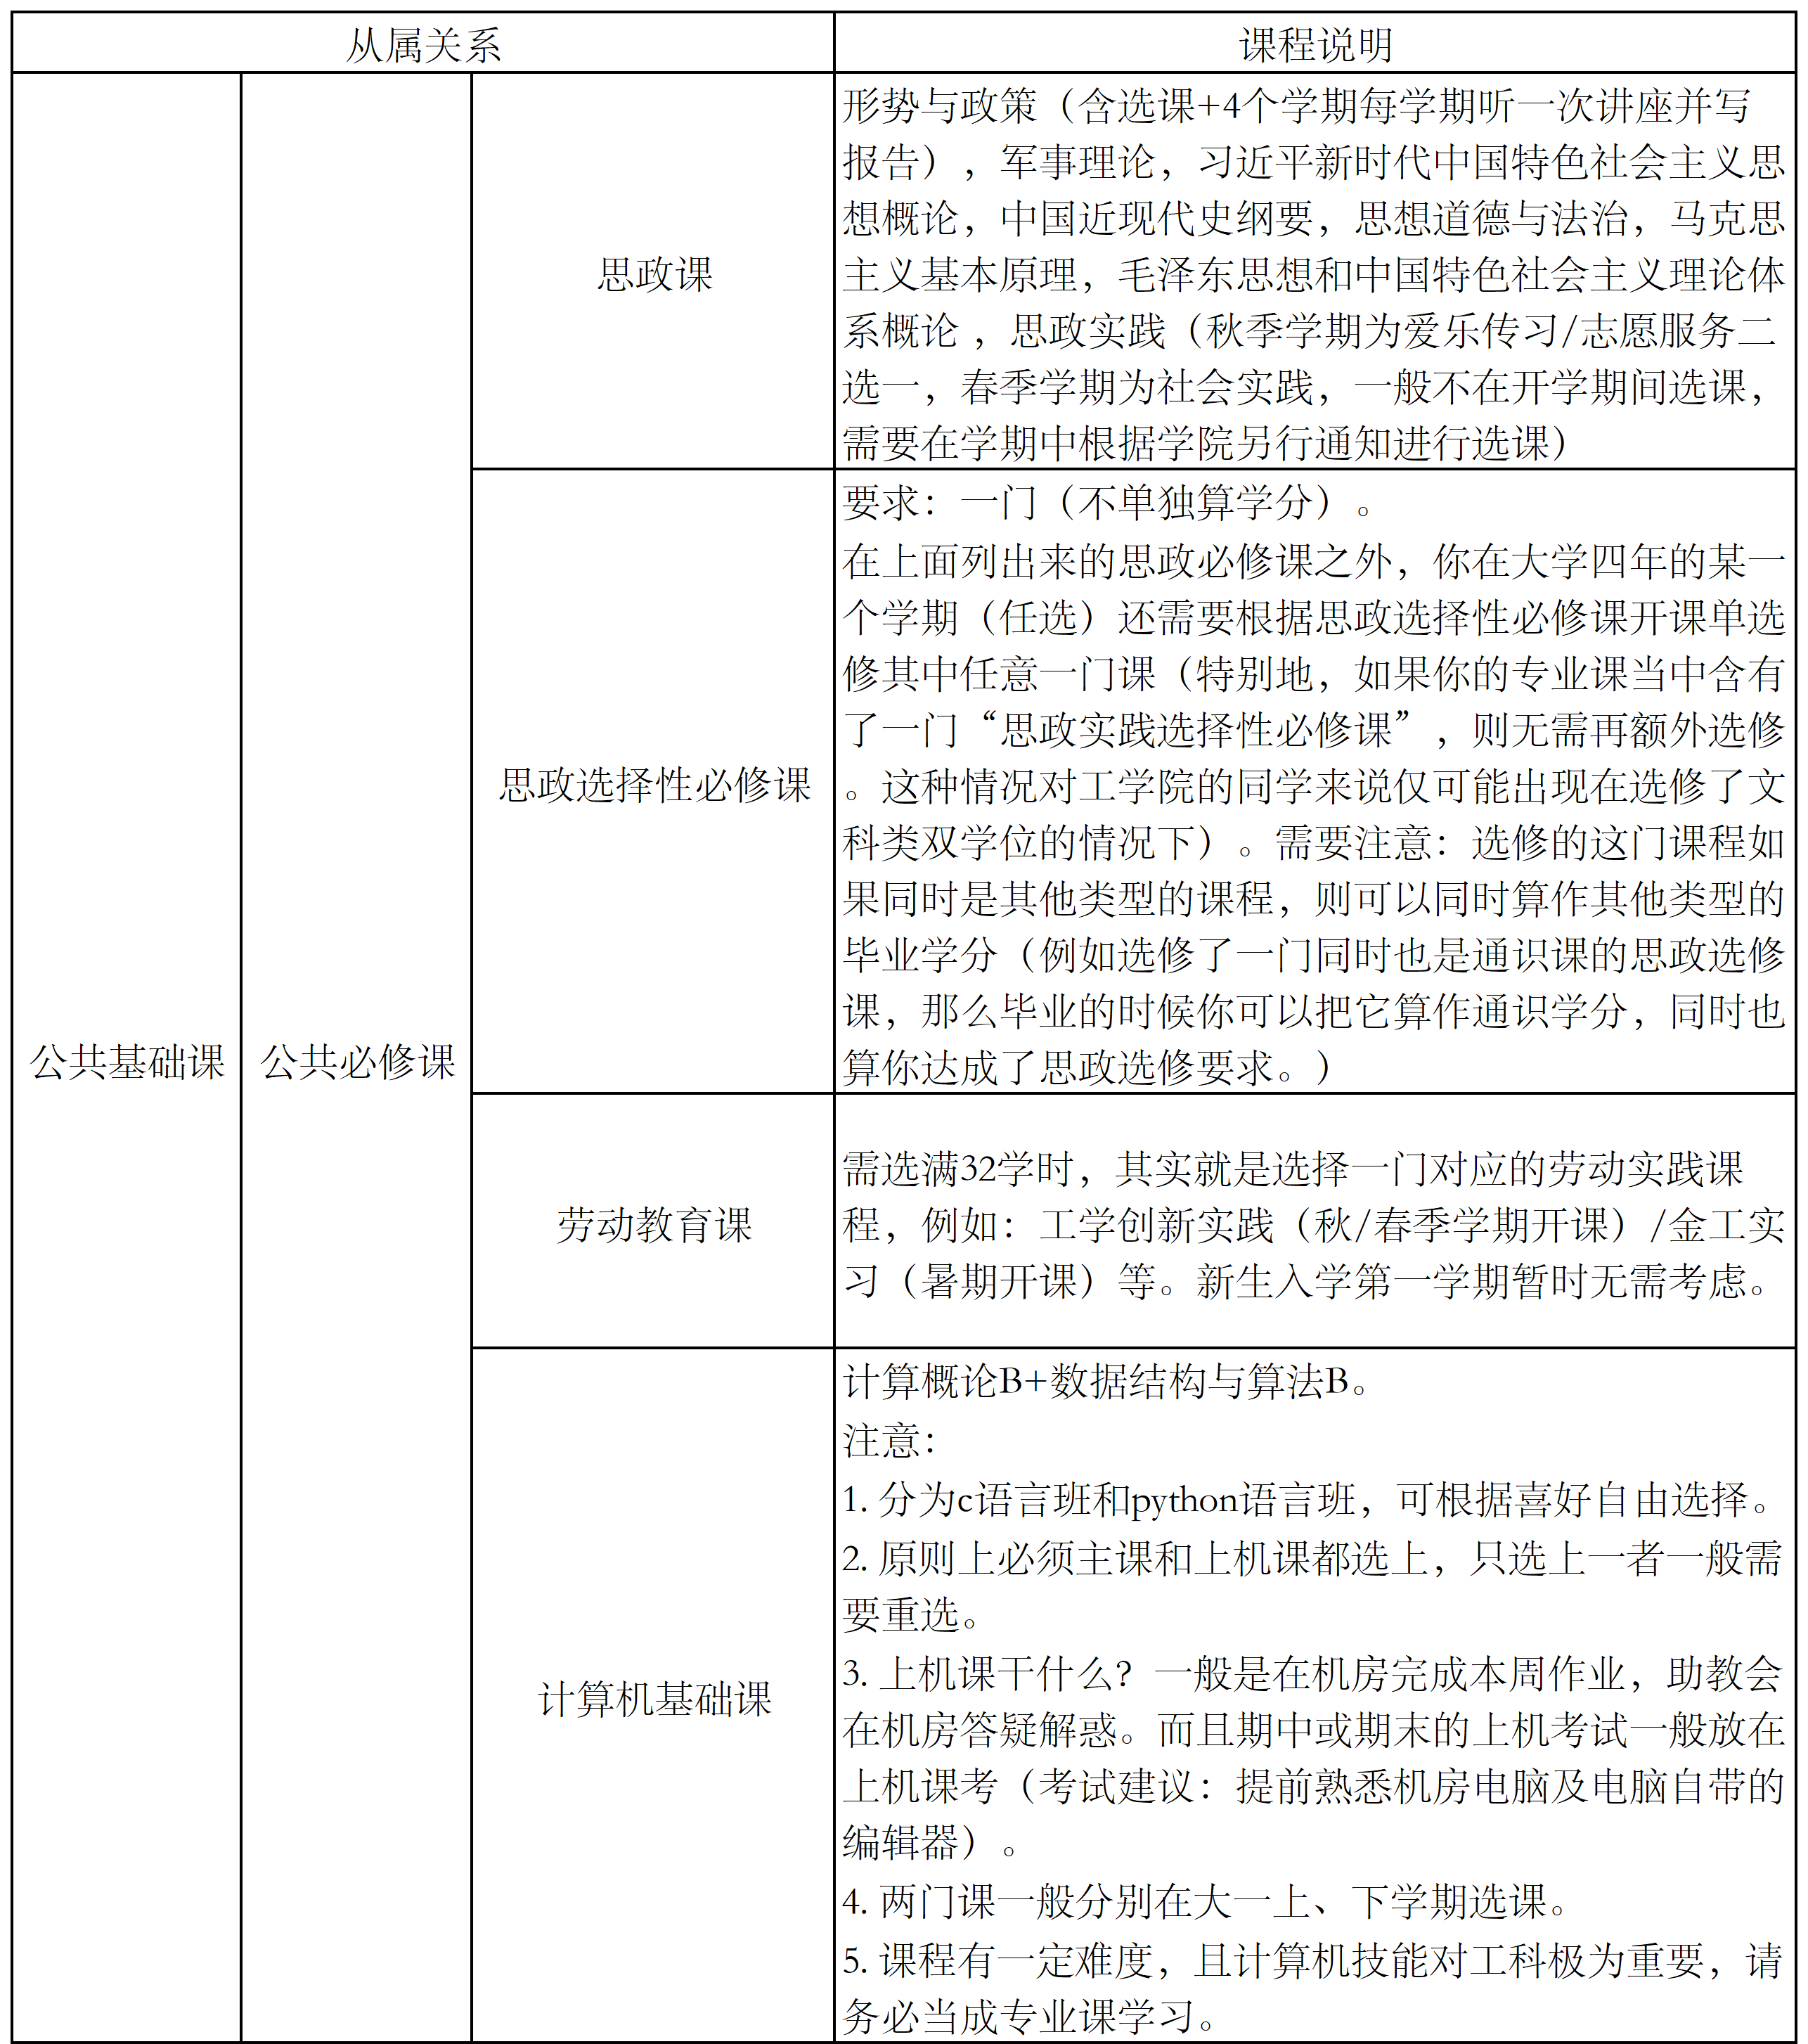
\includegraphics[width=1.02\linewidth]{assets/大表1.png}
\end{figure}

%%%%%%%%%%%%%%%%%%%%%%%%%%这里有个大表格
\begin{figure}[H]
	\centering
	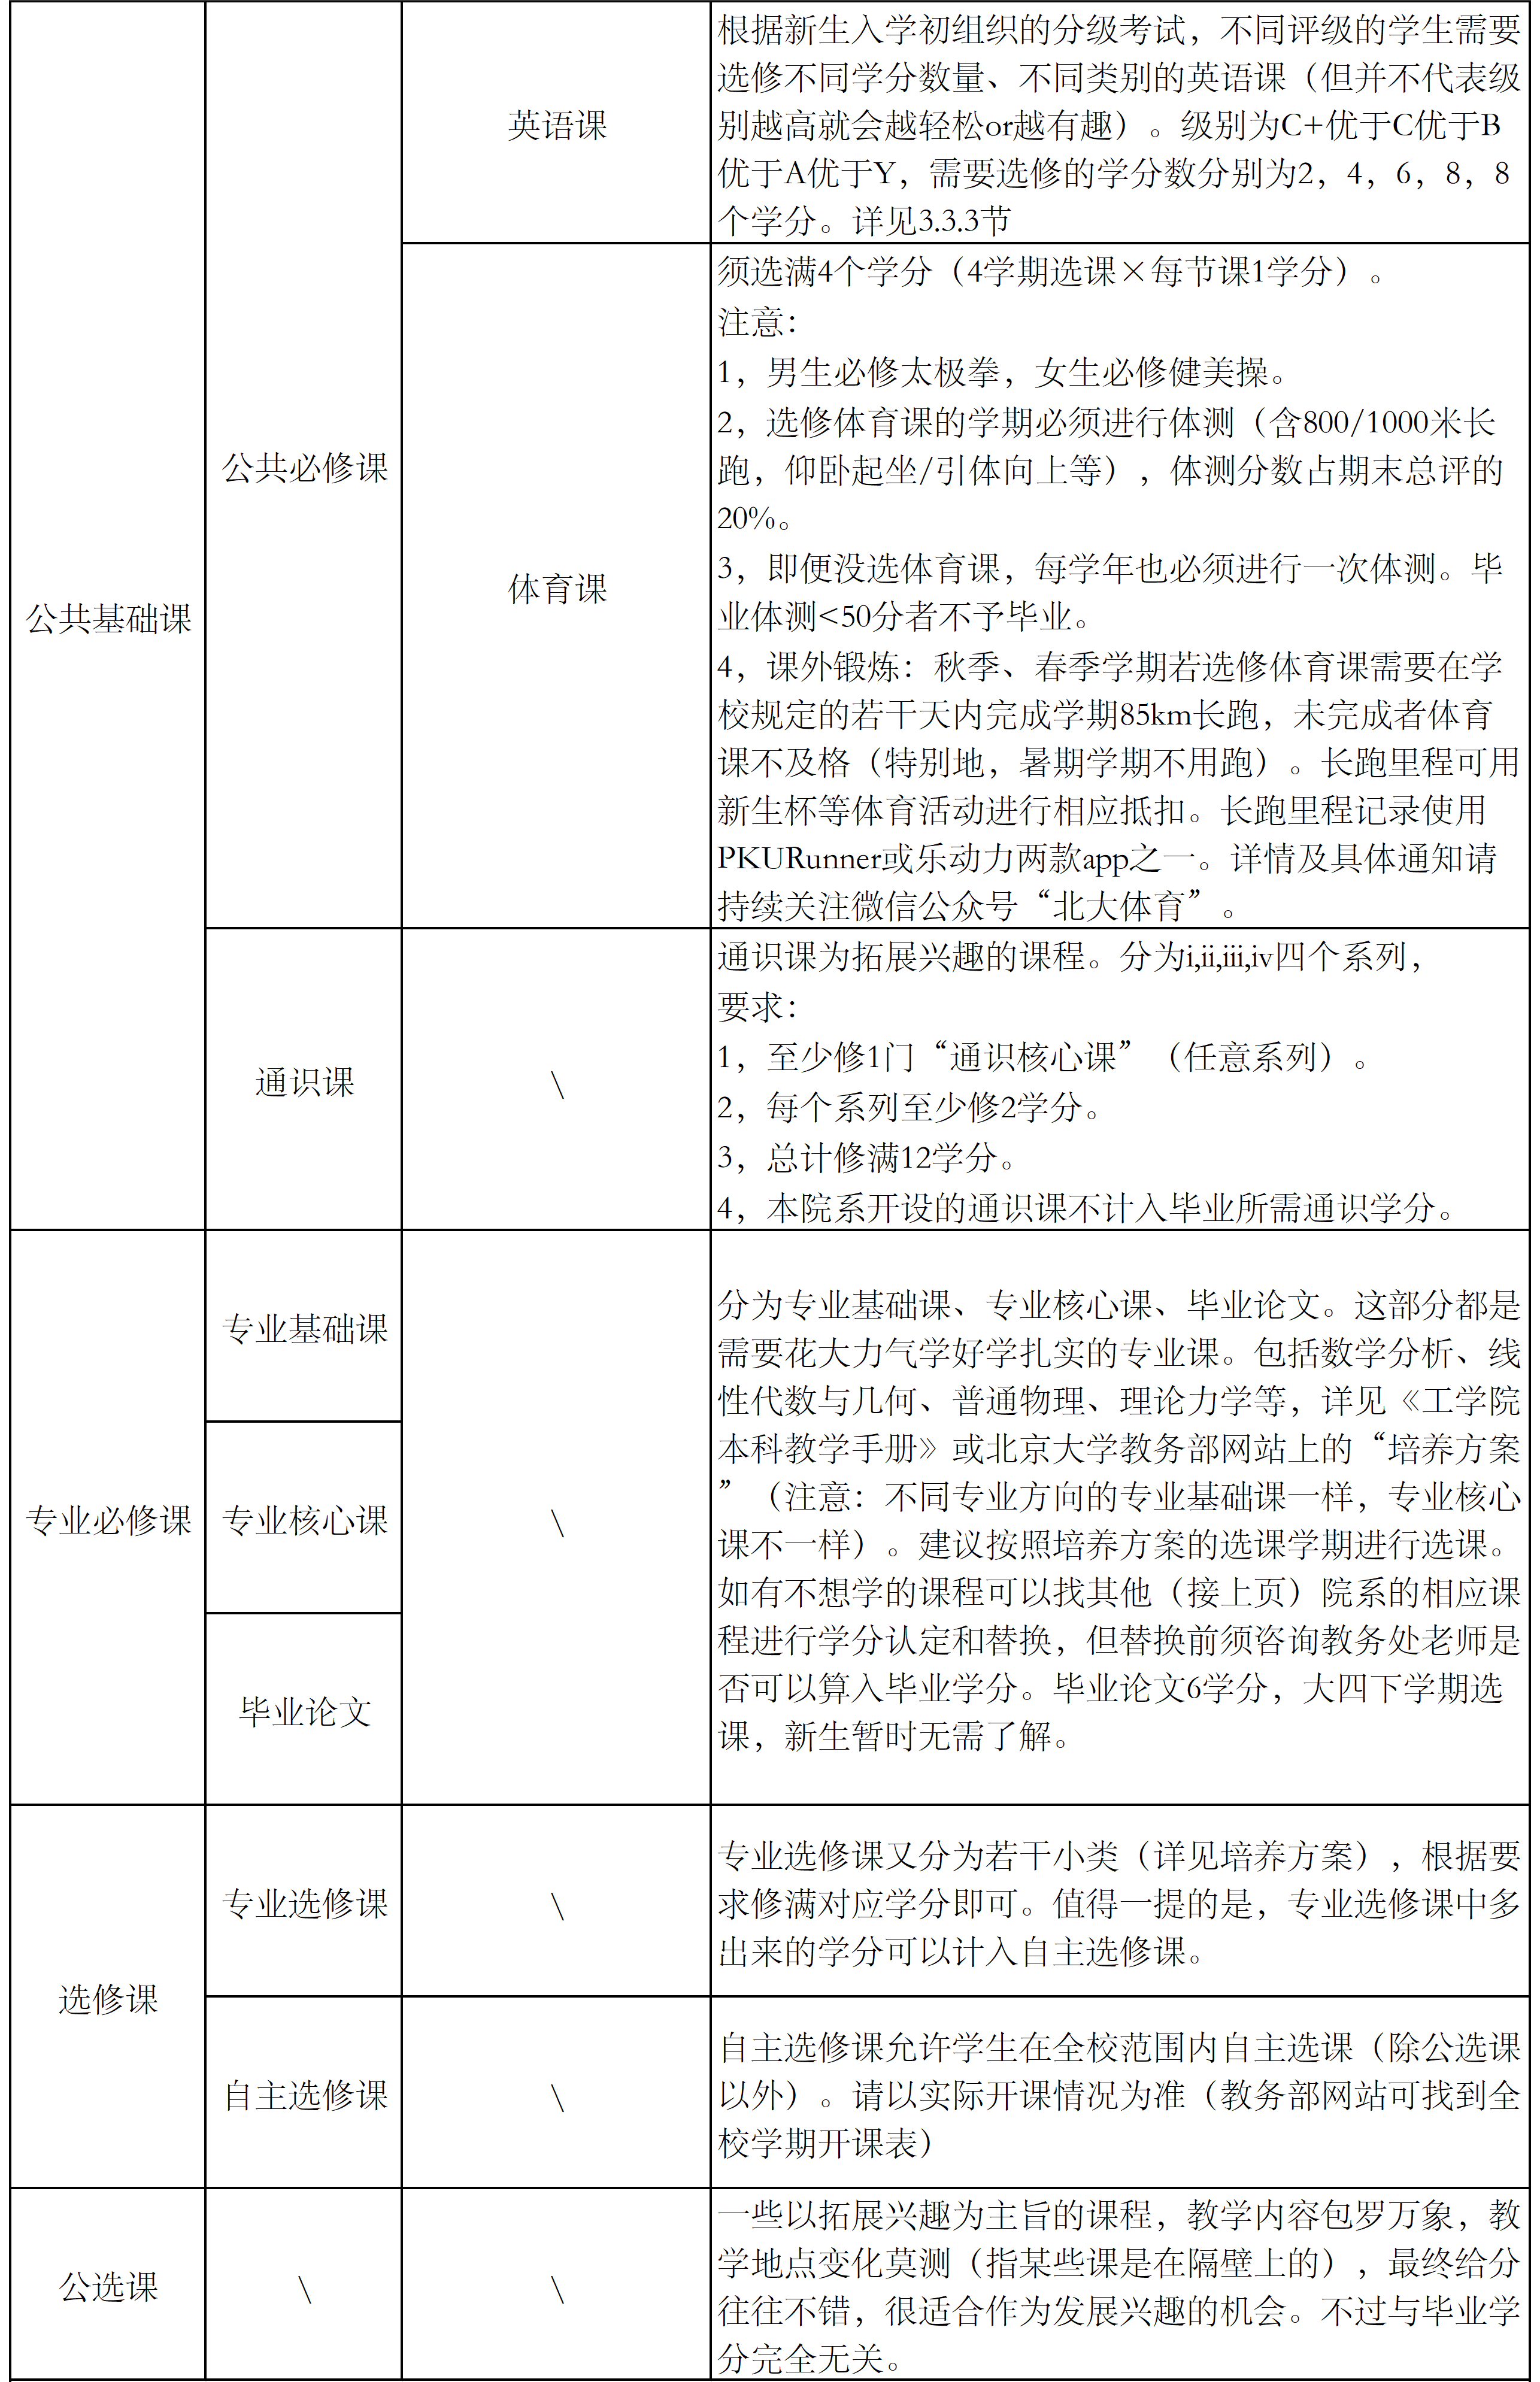
\includegraphics[width=1.02\linewidth]{assets/大表2.png}
\end{figure}



总结：
\begin{figure}[H]
	\centering
	
\includegraphics[width=0.2\linewidth]{assets/2.1.1衡量.png}
\end{figure}

\section{毕业要求}
1. 毕业要求：

修完培养方案中要求的学分，或经教务部审核认定的可以转化的学分。

\vspace{10pt}

2. 推免（保研）要求：

原则上在大三前修完专业必修课和大部分专业选修课，各专业存在差异，详见培养方案。强基和非强基同学要求有所不同，详见1.2.2节

\vspace{10pt}

该部分仅为获得免试研究生资格的必要条件而非充分条件，录取要求请见招生单位相关规定。各专业、各录取单位存在差异，详见培养方案。

3. 荣誉学位要求：

考虑政策变化，具体请参考学院评定细则。

\section{选课网基本操作}

欲进入选课系统，可从北京大学个人门户进入，也可在搜索引擎直接搜索“北京大学选课系统”。下面将以时间为主要线索，对北京大学选课系统（海淀大赌场doge）进行简要说明。

选课总体上分为五个阶段，分别是\textbf{\textbf{预选、补退选第一阶段、补退选第二阶段、补退选第三阶段、补选}}。又可以简单地根据预选抽签前后把时间划分为两个阶段，前一个大阶段（预选）是主要\textbf{\textbf{选课}}阶段，后一个大阶段（补退选和补选）是主要\textbf{\textbf{抢课}}阶段。

\vspace{10pt}

整体时间轴（具体日期每年不同，需要关注教务通知，尤其是暑假学期选课）以2026年秋季学期为例：
\begin{figure}[htbp]
	\centering
	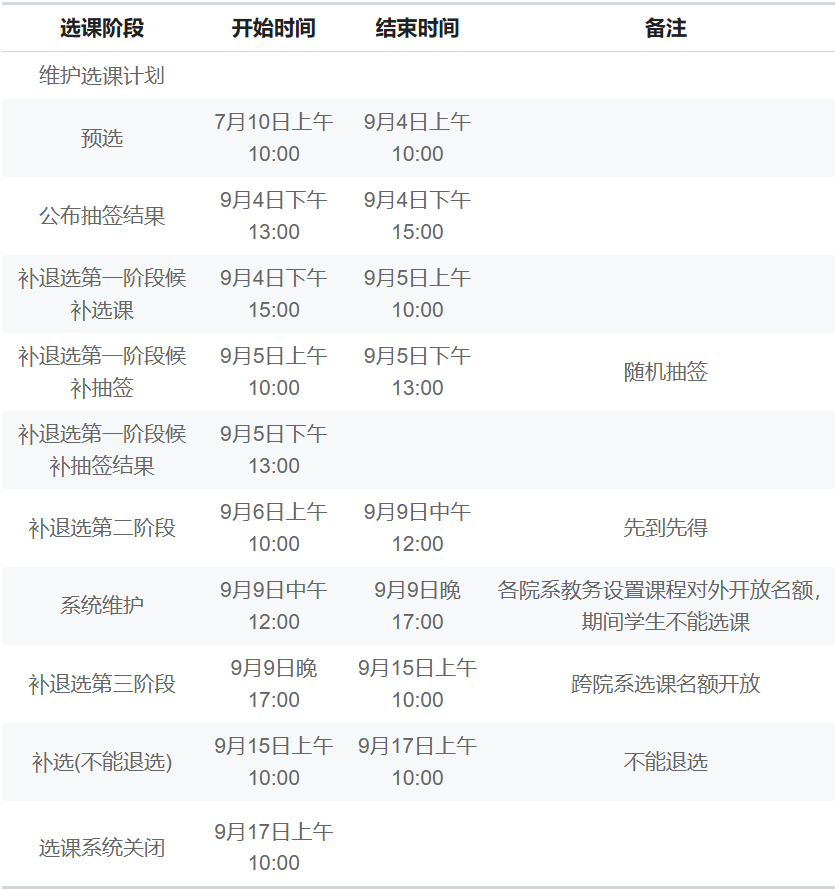
\includegraphics[width=0.6\linewidth]{assets/选课时间轴.png}
	\renewcommand{\figurename}{图}
	\caption{2026年秋季学期选课时间轴}
	\label{fig:enter-label}
\end{figure}

\vspace{10pt}

\textbf{1. 预选}

(1)把课程从选课列表（货架）添加到选课计划（购物车）。

教务会将一些重要课程提前加入选课计划。课程加入选课计划后还没有成功预选。点击课程名称，可以获悉课程简介、所用课本、课程大纲等信息。不过很多信息并不完全准确（有的甚至是十几年之前写的版本），具体内容务必咨询开课老师、学长学姐们。

\vspace{10pt}

(2) 把选课计划（购物车）中的课程添加到预选单（待“支付”）中。

\vspace{10pt}

(3) 为预选课程投点（详见2.5.1节）。

\vspace{10pt}

(4) 等待抽签结果，查看课程是否成功选上。

\vspace{10pt}

\textbf{2. 补退选第一阶段}

从此阶段开始，选课操作需要手动填写验证码以防作弊，每次选课或刷新后均需要填写。

\vspace{10pt}

(1) 如果有人退课，会让出该课程的若干名额，在课程栏显示为xx/xx。

\vspace{10pt}

(2) 把课程加入补退选单中，具体操作和预选阶段基本相同。

\vspace{10pt}

(3) 等抽签抢空出的名额。通常而言几率不大，常常是几十个人抢几个名额。需要提醒的是，教务在补退选第一阶段扩充的名额，会在时间截止前显示在课程栏中。若临近截止时间仍未显示，则大概率不会再扩充名额。

\vspace{10pt}

\textbf{3. 补退选第二阶段}

抢课最关键的阶段，\textbf{先到先得，不抽签}。

\vspace{10pt}

(1) 蹲点等其他同学退课，刷新选课网站以获得空余名额。退课和名额刷新往往不会同步。

\vspace{10pt}

(2) 拼手速抢！具体操作和预选阶段基本相同。

\vspace{10pt}

\textbf{4. 补退选第三阶段}

\vspace{10pt}

(1) 跨院系选课名额开放，可以选一些其他院系的课程。该阶段对于有志于转专业的同学来说比较重要。

\vspace{10pt}

(2) 抢课规则同3。

\vspace{10pt}

\textbf{5. 补选}

\vspace{10pt}

(1) 该阶段选中某一课程后不可退选。

\vspace{10pt}

(2) 可以恳求开课老师收留，或者恳求教务老师增加选课名额。该方法需要灵活使用。

\vspace{10pt}

\textbf{6. 投点技巧}

此处介绍选课投点技巧\footnote{虽然并不是很重要}。

\vspace{10pt}

每位同学一共有99点意愿值，需要在不同课程之间分配。对同一门课程而言，在其他条件均相同的前提下，投点越多的同学，选中该门课程的概率越大。当然，若课程特别火爆，则可能有99意愿值仍然失利的非酋；反之，也可能有0意愿值上岸的超级欧皇。那么，我们该怎样分配点数呢？这时我们需要考虑两个问题：\textbf{什么课程需要投点；投点的课程要投多少点}。

\vspace{10pt}

\textbf{什么课程需要投点：}

\vspace{10pt}

我们已知，对于专业课，比如理论力学方向大家一定要学的数学分析（一），开放名额一定大于对应年级的总人数；且无论如何，教务老师会保证同学们选上本专业的专业课。那么，这门课完全没有投点的必要——事实上系统中也投不了点，因为专业课等会被设置为系统推荐课程，无需投点。什么课需要投点？答案是各类供不应求的体育、通识、英语、政治等。

\vspace{10pt}

我们又知道，一般而言，每位同学每学期最多可以选25学分的课程。这其中专业课占了很大一部分。这就导致了一个问题：若某位同学想预选多门通识课作为备选项，但是发现无法将所有备选项加入预选，否则会超过学分上限。这时可以如下取巧：在预选阶段，不选之后一定会选上的专业课，用专业课的学分空档预选那些通识课备选项。待选上心仪的通识课后，把其他没选上的备选课退掉，再在补退选阶段把专业课加回来。这是一种小技巧，更多技巧建议自行体悟。

\vspace{10pt}

\textbf{该课程投多少点：}

\vspace{10pt}

比较热门的投点办法有两个：质数投点法（玄学）和all-in投点法。前者认为，只要所有投点都是质数，则最终选课成功率大大上升。后者不计代价地把大量点数\footnote{甚至所有点数}砸到一门课中，以期待高概率选中一门课。

\vspace{10pt}

后一种方法未必不好，因为这至少保证了一门好课大概率选中。当然，也有可能all-in但仍然选不上orz。如果我们采取平均投点的办法，每门课选中概率都不大，有可能出现所有课全都选不上的情况，但也有可能全中。最终的投点办法，还需自行衡量。有一个有意思但未必有用的投点辅助程序可以玩一下。\href{https://wyjjmzx.github.io/pku/toudian.html}{https://wyjjmzx.github.io/pku/toudian.html}

\section{选课信息来源}
我们常用以下途径判断一个课程的综合好评率：

\vspace{10pt}

1.在选课网的“选课计划”中，点击课号或课名，可以查看课程的先修课程、简介、大纲、教学评估得分等信息。其中教学评估是每位同学在临近期末考试时给课程做出的评估。选课网上的信息主要来自老师、助教、教务等，相对注重课程的内容部分，也更正式，而以下四种渠道的信息则更多来自同学。

\vspace{10pt}

2. 看“预选名额/计划名额”。本质上是直接应用他人劳动成果。其他同学搜索了解该课程后觉得不错，因此预选人数较多，那大概率这门课的综合口碑不错。

\vspace{10pt}

3. 树洞treehole.pku.edu.cn，搜索课程简写或老师姓名简写即可查到学长学姐的课程测评。考虑到树洞的匿名性质，课程评测等内容需要同学们注意分辨。

\vspace{10pt}

4. 非官方课程测评网站。在搜索引擎中直接搜索“北大课程测评”，第一个网站即为课程测评网站。该网站完全非官方，且完全不控评，内容同样地需要同学们注意分辨。

\vspace{10pt}

5. 广泛咨询靠谱的学长学姐，获得较为详细的听课感受等信息。

\vspace{10pt}

\textbf{核心要义：不仅仅追求良好的给分，更要追求自身兴趣能力的发展。}

\section{特殊选课模式}
\subsection{跨院系选课}
有志于转专业、双专业、辅修的同学需要注意，其他院系的专业课只可在补退选第三阶段进行选择。因此，需要提前为想选的课预留出时间和学分空间。

\vspace{10pt}

如果没有转专业、双专业、辅修打算，也可以在这一环节选择其他院系感兴趣的课程。学分可计入毕业学分中的“自主选修课”部分。

\subsection{课程替代}
培养方案是灵活机动的。根据培养方案，一些课程之间可以互相替代，进行毕业学分认定。关于培养方案上未明确的内容，请主动咨询工学院教务老师。

\subsection{冲突选课和手工选课}
申请特别麻烦，且一般用不上。若实在需要可参照：教务部网站-学生-选课和退课。

\subsection{双学位选课与超学分选课}
分为主修+辅双两个选课通道。辅双通道可以进行双专业、辅修课程的选择，且无需投点。通过辅双通道选择的双学位课程需要缴纳相应学费\footnote{详见本手册4.1}。

\vspace{10pt}

理论上，每学期选课量为14$\sim$25学分。当挂科不超过两门时，可以申请超学分选课，一般至多为每学期30学分。超学分选课需要经历一系列申请、审批过程，详见教务部官网。

\vspace{10pt}

特别地，双专业学生选课每学期学分上限为30学分。

\subsection{中期退课}
每学期中期\footnote{第八周左右}可根据教务通知进行中期退课。

\vspace{10pt}

体育课，第10周之前已经结束的课程，以及物理、生物、化学类实验课不允许中期退课。因病等特殊情况需要退体育课的同学，须提供由任课教师以及体育教研部主管教学的领导签字同意的《北京大学本科生手工退课申请表》，在退课期间交至体育教研室教务办公室（五四体育中心203），逾期将不予受理。

\vspace{10pt}

退课后，成绩单上该课程记为W，不参与绩点计算。退课后每学期所修学分一般不得低于14学分下限。

\vspace{10pt}

中期退课是某一门课程实在学不下去时的应急策略。过多的中期退课可能会让老师对学生的能力产生质疑。同学们可以适当使用，但不建议过度依赖。

\subsection{绩点改革}
以下内容依据教务部《关于进一步做好本科学业评价工作的通知》。该文件发布于2025年7月25日。

\vspace{10pt}

改革的具体影响如下：

\vspace{10pt}

1.从2025年秋季学期开始，每学期第九周结束前，同学们可在部分公共基础课程和专业课程包以外的课程内选择1门课，以“合格制（P/NP）”方式记载成绩。

\vspace{10pt}

2.允许课程等级制给分，取消课程优秀率限制。

\vspace{10pt}

3.从2025级开始，在各项含有学业评价的工作中不再使用绩点，而使用完整成绩单。

\vspace{10pt}

其中，笔者认为有几点需要着重：

\vspace{10pt}

1.百分制成绩与等级制成绩没有直接转换关系。

\vspace{10pt}

2.部分公共基础课程（包括大学英语、思想政治理论必修课、信息课程、军事理论、体育课），主修专业的专业必修课及院系特定课程不得采用P/NP方式记载成绩。也就是说，大一的大家可以选择P/NP方式的课程主要是通识课。

\vspace{10pt}

3.更关注于专业课的成绩排名。

\vspace{10pt}

4.如果按均分制计分，相比绩点制来说，低分课程的影响没那么大（绩点制下，任何一门<70分的课程对绩点都是灾难性打击）

\subsection{不按照培养方案选课}
理论上，同学们可以有自己的选课规划。但需要指出的是，培养方案的设置有很大的合理性，适合绝大多数人的学习进程。如果想按照自己的节奏安排课程，建议与老师、学长学姐深入探讨一下这种方案的合理性。

\chapter{学习生活}
\section{工学院培养方案}
探索过工学院官网的同学可能会发现，工学院近几年的培养方案几乎是一年一改，辅修双学位的政策也时有变动。笔者认为，这与2019年开设机器人工程专业、2020年录取强基计划的学生、近年来学院课程开设情况、同学诉求等诸多因素有密切关系。

\begin{figure}[htbp]
  \centering
	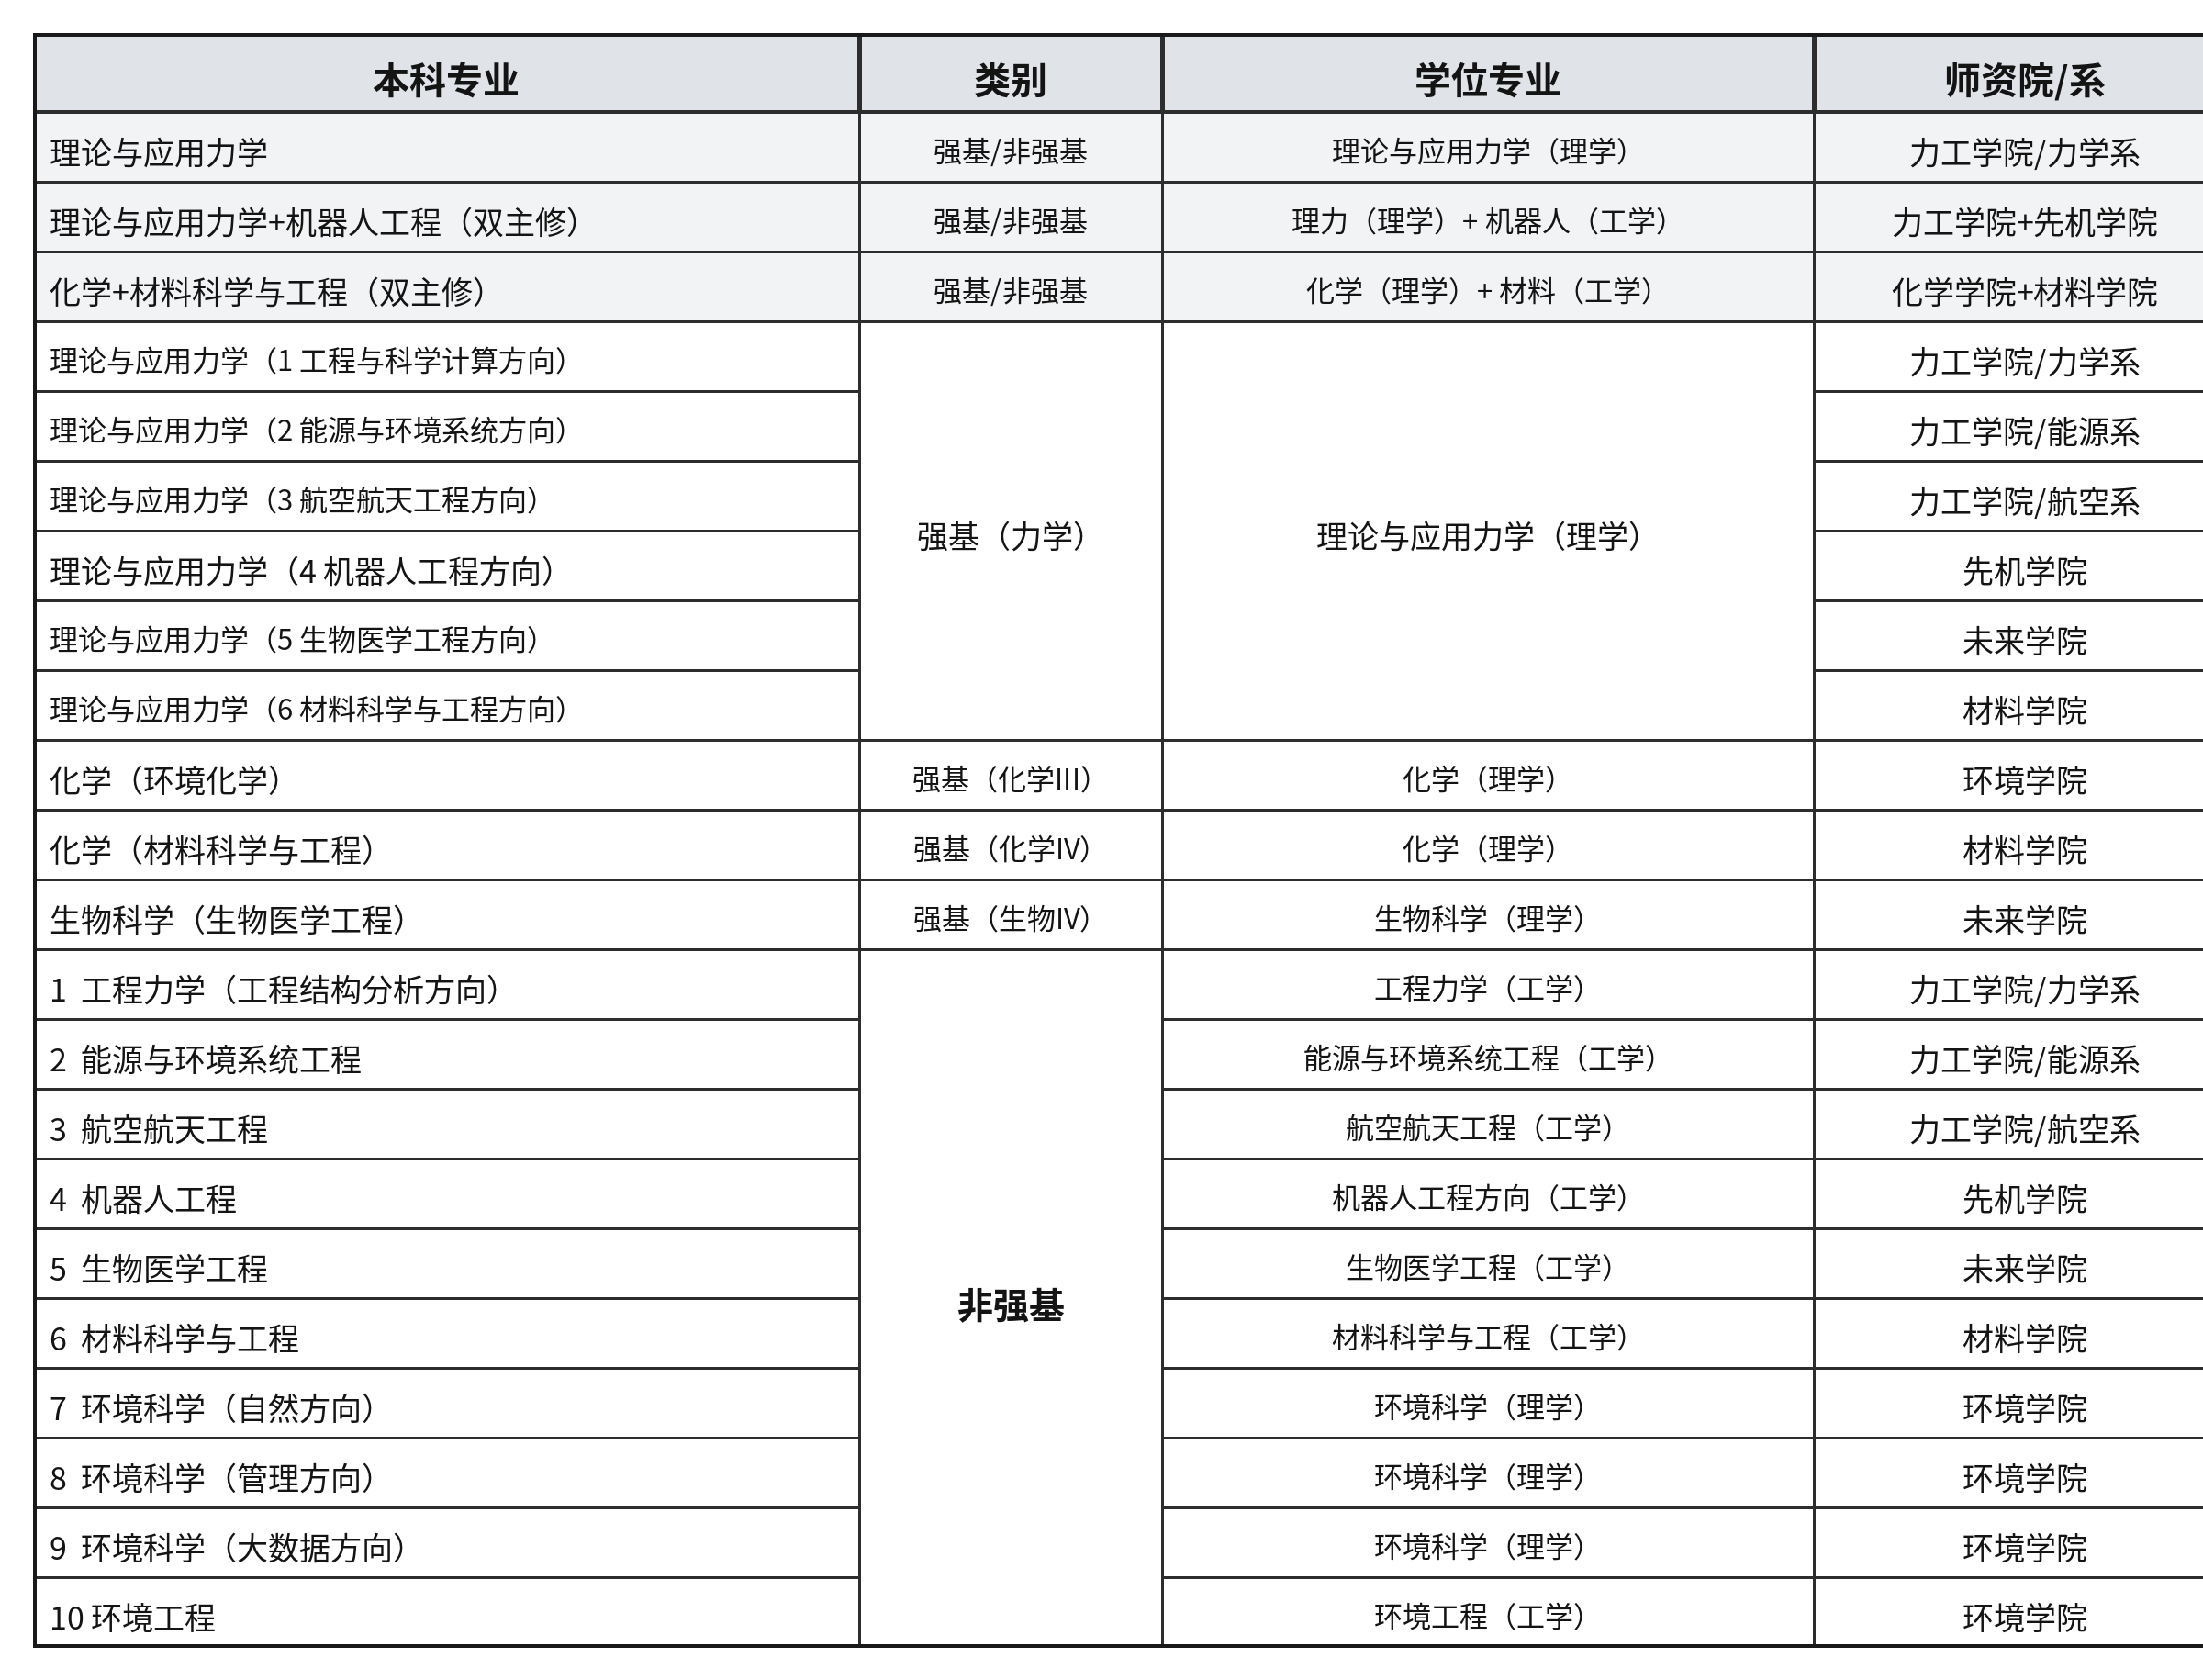
\includegraphics[width=1\linewidth]{assets/培养方案.png}
	\renewcommand{\figurename}{图}
	\caption{2024版培养方案专业情况}
	\label{fig:enter-label}
\end{figure}

\vspace{10pt}

数百位思想意识独立、成长环境各异、未来规划多种多样的本科生，若全部严格遵循一份名为“培养方案”的小册子中的表格与条款，必然导致毁灭性的结果。正如一位厨师为一千人炒一大锅菜，我敢说我夹到的那部分大概率不是夹生就是糊掉。

\vspace{10pt}

因此，阅读培养方案时，大家应时刻主动思考：我希望培养自己的哪些能力？培养方案能在哪些方面帮助我？学院暂时帮不到的方面我该如何自己找办法？希望大家辩证看待课程安排，逐渐学会分析培养方案现存的不足，取其精华，去其糟粕。

\vspace{10pt}

笔者分享自己的一些见解供大家参考。在理论学科领域一直以来的优势地位，使得北京大学在新工科发展上选择了“以科学促工程”的思路，这一思路也直接反应在了工学院的培养方案上：重视理论教学，而实践、设计、研发、创造类的培养较少。显然，工学院培养方案给予同学们最大的优势就是坚实的数理基础——各类注重理论的专业课为大家建构学科知识体系，同时在学习过程中包含了不少练习和考试。因此，认真学下来，大家会收获极为宝贵的逻辑分析能力。以数学分析为例，其本身就蕴含长逻辑链条的知识脉络，很多推导和证明也都是环环相扣；物理类课程可以训练大家的建模能力，将现实生活中的复杂问题简化抽象为可以解决的数学模型。这些能力会让我们在之后的学习和研究中更有条理、更加深入地考虑问题。

\vspace{10pt}

现行培养方案亦有难以避免的核心问题：内容难度和抽象程度较高，课程数量较多。

\vspace{10pt}

一方面，大家容易停留在抽象层面上沾沾自喜，忽视了抽象的理论知识和具体的现实问题大相径庭。如果只掌握抽象的知识，或者一些近乎炫技的解题手段\footnote{除了得分，解题手段在大学没有任何价值可言，而分数在你毕业后只是一串数字}，却不注重实际应用，那么抽象理论对于大家则毫无价值可言。这种在实例中应用的训练恐怕需要通过实实在在的大作业和科研训练来完成。对于前者，部分老师的课程含有大作业，大家可在树洞上善用搜索，在选课时予以关注考量；对于后者，大家可以通过本科生科研\footnote{一般在大二开始，少数同学会在大一下学期开始}锻炼自己。

\vspace{10pt}

另一方面，我们不可忽视时间成本。难度较高、数量较多的理论课程，想要学好、学透它们，是需要相当多的时间的。现在的大环境下，本科生进行科研训练，对于升学和选择研究生导师都是十分重要的。缺乏类似训练，势必会对后两者造成影响。而课程的难度和数量，在某种程度上对于大家及时进入科研训练是一种阻碍。

\vspace{10pt}

总而言之，工学院培养方案正在不断迭代中逐渐改进，但问题总归会有。方案本身只是一碗最为基础的大锅饭，加上什么样的菜拌着吃，是大家接下来需要认真辨析和思考的地方。

\section{基础课程}
\textbf{强调：}

以下内容为编写团队一己之见，具有一定参考价值。但我们也鼓励大家去别处，如认识的老师、学长学姐以及树洞等，寻求解答。希望大家兼听则明，敢闯敢试，探索出一条适合自己的学习之路！

\vspace{10pt}

我们还要提醒大家：学会探索属于自己的学习方法。到大一下学期，大家应该尝试着摸索，如何从了解到学好一门课程。同时切忌平时偷懒——习以为常的不了了之会导致后面越来越听不懂，引发“雪崩效应”。

\subsection{数学课程}
\textbf{1. 数学分析（一）（或：高等数学（I））}

数学分析，是一门以微分、积分为核心而展开的一系列强调“逻辑”“精确”的分析式课程。教材推荐张筑生老师的《数学分析新讲》\footnote{亦称其为“黄皮书”}，网课推荐b站上史一蓬老师的数学分析公开课。

\vspace{10pt}

笔者对于学好数学分析（一）的建议如下：

\vspace{10pt}

（1）注重“极限”“连续”“可导”“可积”等基本概念的书写，“中值定理”“泰勒公式”等定理公式的使用条件。解答习题时力求完整、严谨书写，拒绝伪证。事实上，能敏锐地发现伪证的漏洞，说明你对于概念和定理的掌握已经非常牢靠了。因此，我们建议考前进行一些有关基本概念和定理公式的系统整理记忆。

\vspace{10pt}

（2）证明题没有思路时可以尝试结合图像或题目条件进行思考，搭建大致思路后再用严谨的语言（如$\varepsilon-\delta$语言）书写。切忌一蹴而就，这样往往会导致思路混乱、漏洞百出。

\vspace{10pt}

（3）无需完全掌握一些过于复杂的证明，只需知晓大概思路即可。事实上，考试一般不会涉及这类高难度的证明，而很多新生容易在这上面花太多时间，导致整体逻辑框架混乱，重点偏移。

\vspace{10pt}

（4）鉴于数学分析极易因“想当然”而出错，掌握若干经典且基本的“反例”显得尤为重要。

\vspace{10pt}

（5）利用好习题课，多和老师、助教、同学探讨交流，互相体会对方证明或解题过程的优点和不足\footnote{也有可能发现对方是伪证（doge}。

\vspace{10pt}

\textbf{2. 数学分析（二）（或：高等数学（II））}

进入大一下学期，数学课程难度会陡然上升，你会觉得“上学期学得这么简单，但我竟然还喊不会！”这其实说明，你的水平上涨了许多。事实上，当你在学习某一课程中，感觉过程不快但又并不至于崩溃时，往往是水平上涨最快的时候。不必担心，时间会证明一切。

\vspace{10pt}

数学分析（二）会逐步介绍广义积分、多元微分，多元积分。内容看似简单，实则丰富且变化多端，尤其是多元微积分部分。因此，我们建议课前适当预习，否则容易上课走神导致整节课跟不上\footnote{笔者曾不幸体会，简直是巨大的灾难}；同时，课后认真总结和完成习题。此外，我们需要强调史一蓬老师的教学思想之一：问题不过夜。考虑到数学类课程具有极强的前后关联性，未及时解决的问题积累下来会导致后续内容学得云里雾里。因此，请大家尽量做到“今日事，今日毕”，或者至少“本周事，本周毕”。

\vspace{10pt}

具体学习建议和数学分析（一）大致相同，建议投入更多的时间和精力，适当增加练习量。

\vspace{10pt}

\textbf{3. 线性代数与几何} 

线性代数与几何，是一门介绍矩阵与行列式运算、线性变换、向量与几何为核心的课程，在多数人眼中，难度高于数学分析（一）。教材推荐David.C.Lay的《线性代数及其应用》（Linear Algebra and Its Applications），上手容易，框架清晰，70\%习题很简单，且很多题目里暗藏玄机\footnote{指暗含很多高等代数的知识，极具启发性}。如能读完本书，必定收获颇丰。

\vspace{10pt}

笔者对于学好线性代数的建议如下：

\vspace{10pt}

（1）构建思维导图，知道若干概念对应若干性质\footnote{例如“可逆矩阵定理”的24种表述}，便于后期融会贯通。

\vspace{10pt}

（2）认真完成作业，力求算得又快又对，在作业中总结方法技巧。核心知识往往只能在实际操作即做题中掌握。

\vspace{10pt}

（3）掌握基本定理的证明，因为证明中的思想和技巧能帮你更深入了解定理的来龙去脉，而且很容易用在具体的题目当中。

\vspace{10pt}

（4）多交流多探讨。线性代数往往会在周末开设“学业辅导课”，由高年级学长学姐或课程助教讲授，基础与拓展均有涉及。如有兴趣，可以一试，以进一步夯实数理基础。

\vspace{10pt}

\textbf{4. 高等代数}

如果你把线性代数学得特别通透，那么高等代数大概率不在话下。高等代数的核心知识和线性代数基本一样，会额外增添多项式理论、线性空间和空间上的线性变换、若尔当标准型等重要内容。教材推荐丘维声老师的《高等代数》\footnote{数院所用教材，部分章节无需掌握。至于是哪一部分，见仁见智，请听好老师的安排与学长学姐的建议}。

\vspace{10pt}

笔者对于学好高等代数的建议如下：

\vspace{10pt}

（1）敢于去繁从简。很多证明思路繁杂，技巧性强，没精力也没必要掌握。但是同样地，你应该知道它的核心思路；亦不可忽略包括但不限于老师所强调的、地位关键的证明。

\vspace{10pt}

（2）多角度理解一个定理到底在说什么，换而言之，把知识串起来。例如：限制线性变换和矩阵对角化的联系、最小多项式的多种求法等。

\vspace{10pt}

（3）多做题但不盲目做题。计算是工院人最基本且核心的技能。因此，我们需要掌握各种跟“算”有关的思想方法和技巧，在此基础上再去掌握证明（也会相应地变简单一些）。

\vspace{10pt}

\subsection{物理课程}
\textbf{1. 普通物理（I）}

普通物理是大家正式接触的第一门物理类课程，开课时间为大一下学期。普通物理（I）包含力学、电磁学的大部分基础内容，且两者往往以期中考试为界限分开。教材推荐钟锡华老师、陈熙谋老师的《大学物理通用教程》。

\vspace{10pt}

对于有一定物理竞赛经历的同学而言，普通物理课程几乎所有内容都是“已学习”状态。因此，笔者推荐《物理学难题集萃》（舒幼生、胡望雨、陈秉乾）作为拓展材料。

\vspace{10pt}

笔者对于学好普通物理（一）的建议如下：

\vspace{10pt}

（1）熟练掌握教材中的基本概念和经典模型，熟练程度决定解题速度上限。

\vspace{10pt}

（2）先自行完成习题，再看答案。期中或期末考试的部分题目来源于作业和往年题，平时直接照抄的一时之快，最终只会化作考场上的抓耳挠腮，得不偿失。

\vspace{10pt}

（3）进行适当拓展。受限于课时和班级人数，普通物理课程难度中等，所讲授的内容存在一些不够深入的地方，等待大家通过阅读进阶材料\footnote{老师可能会在课上列出进阶教材等。若没有，请善用搜索}等方式自行探索，构建更为完善的知识体系。

\vspace{10pt}

\textbf{2. 普通物理（II）}

开课时间为大二上学期，介绍热学、光学和近代物理三部分内容。教材仍为《大学物理通用教程》，不同老师授课进度和内容选取不尽相同。

\vspace{10pt}

笔者认为，相比普物（I），普物（II）内容更多、更注重理解，因此给出下列学习建议供大家参考：

\vspace{10pt}

（1）阅读教材多多益善，理解物理概念和物理过程。有余力可参阅其他教材，相得益彰。

\vspace{10pt}

（2）反复推导重要公式、结论，直至没有疑点。这能在解题时帮你节省相当一部分时间。

\vspace{10pt}

（3）抓大放小，关注主干内容。同样地，受限于课时等因素，教材中存在众多介绍类内容，且该部分内容在后继物理课程（如热力学与统计物理、电动力学、量子力学、固体物理等）中有严密的理论推导来支撑，所以不必事无巨细地搞清楚每一句话。

\vspace{10pt}

此外，对于普通物理课程，同一课程号的不同班级可互相替代。因此，我们建议大家选课前通过各个渠道，广泛参考不同班级的课程评价，了解工院班与数院班、地空班等不同班级、不同老师的课程侧重和授课风格，选择最适合自己的班级。当然，学有余力、力求进阶的同学可以选修物理学院开设的力学、电磁学、热学、光学、近代物理等替代普通物理。详情请咨询教务老师或参阅培养方案。

\subsection{化学课程}

\textbf{1. 普通化学B}

来到大学，化学课依旧保持了其庞杂、缺乏系统规律的特点。其主要内容是更加深入地讨论很多高中时期悬而未决的问题，比如吉布斯自由能的来源、平衡常数表达式的导出、物质的内部结构等，但难度、知识含量远远大于高中时期。教材推荐北大出版社的《普通化学原理》（蓝皮书）。笔者在此给出下列学习建议，供大家参考：

\vspace{10pt}

（1）搞清楚概念、定义，做到能够自己复述。大学化学中的概念可能对一些同学来说会较抽象，如成键轨道非键轨道等，这就需要同学们自己阅读课本，自己查资料，直到完全弄懂概念。厘清概念是整个化学学习的基石，务必要重视。

\vspace{10pt}

（2）仔细研究老师课堂上给出的例题，要自己独立的做出来，虽然面对复杂问题思考的过程可能很花时间，但对于能力培养和考试成绩都很有帮助。

\vspace{10pt}

（3）掌握多元化的解题方法。课堂上提到的方法尽量都要掌握，也基本都会在考试中用到。 妄图用单一的方法解决所有问题往往会使问题变得更难解决。

\vspace{10pt}

（4）各位上的化学课可能是开卷也可能是闭卷，但不能因为开卷考试就放松警惕，否则很有可能翻遍书都找不到答案。建议按照闭卷考试的要求学习和准备考试。

\subsection{生物课程}

\textbf{1. 普通生物学}

普通生物学B是一门Ⅳ类通识核心课，自24级开始被列为生物科学（生物医学工程方向）的专业课，选课时间为大一下学期。普通生物学B作为一门通识课，一般由佟向军老师或者陈丹英老师开课，其中佟老师的普生B同时是元培同学限定选修范围内的课程，作为生物医学工程同学的专业课的是陈丹英老师的普生B。这门课的教材是《陈阅增普通生物学》，不过其实看老师的PPT就足够了。

\vspace{10pt}

笔者对于普通生物学B的建议如下：

\vspace{10pt}

（1）关注往年题（这点的重要性毋庸置疑）。

\vspace{10pt}

（2）作为一门通识课，该课程的课业压力并不是特别大。大家可以妥善安排时间，例如在学期初完成论文翻译的工作，这样期末周的压力就会相对小。事实上，该思路适用于大多数通识课。

\section{公共课程}
\subsection{计算机基础课程}

计算机基础课程指计算概论和数据结构与算法两门课，分别在大一上、下开课，由信息科学技术学院的老师开课，多个学院同学合上。需注意，不同老师开设不同语言的课程，分为C语言和Python。C语言相对更底层更基础，Python相对更简洁开发效率更高。两种语言不分优劣，请大家自行选择。此外，一门计算机课程由课程本体和上机课两部分组成，大家需同时选择同一班级的上机课。

\vspace{10pt}

笔者认为计算机课程需注意两个方面：理论基础和代码能力。

\vspace{10pt}

理论基础会在笔试\footnote{一般为期末考试}中考察，具体内容包括但不限于计算机原理、网络与互联网基础、信息表示与存储、数据基础、算法思想和程序设计等。

\vspace{10pt}

代码能力会在上机考试\footnote{一般为期中考试，也可能单独考试}中考察，要求使用完全正确的逻辑和算法解决问题。笔试是基础，上机是应用，二者的关系类似于理论与实践，任一方面的欠缺都会影响课程学习，因此在学习过程中不宜偏废。

\vspace{10pt}

很多同学没有信息竞赛基础，或者从来没接触过代码，可能会担心不能适应课程。这样的担心是合情合理的，但也是不必要的。事实上，计算机课程会以0基础为参考水平进行教学，绝大部分同学无需考虑不能适应的问题。如果实在放心不下，可以提前寻找资料学习某一语言的基础语法。

\subsection{思想政治课程}
思想政治课程包含：形势与政策（形策）、军事理论（军理）、中国近现代史纲要（史纲）、思想道德与法制（思修）、习近平新时代中国特色社会主义思想概论（习概）、马克思主义基本原理（马原）、毛泽东思想和中国特色社会主义理论体系概论（毛概）、思想政治实践。

\vspace{10pt}

政治课最终分数一般由以下部分构成：平时分+论文分+考试分，其中考试分是主体，平时分具体打分方法因老师而异，但大多数政治课的大多数老师都会开设小组展示（Presentation）\footnote{简称pre}。大家在学期初进行分组并确认主题，小组内针对课程内容某一部分进行深入探讨，并进行一定时长的课堂展示。由此，政治课的主要任务是：准备小组展示、写论文、准备期末考试。

\vspace{10pt}

对于政治课的期末考试，平时功夫固然重要，但是期末复习尤其关键。由于不同老师讲课风格迥异，课程安排也不尽相同，而每门政治课考试是全校统一考试，因此考试题目不会有很强的个性。这也意味着题目可被穷举，且有很强的模板性。我们推荐大家通过各类渠道\footnote{详见本手册后续介绍}整理复习资料和往年题目，并多次背诵强化记忆。政治课的最终得分和期末复习时背诵的严格程度、完整程度是强正相关的。

\vspace{10pt}

最后，我们介绍思政实践课程。思政实践课程\footnote{详见practice.pku.edu.cn}包括“爱乐传习”“志愿服务”“社会实践”三个模块。“爱乐传习”即一二九合唱比赛；志愿服务如字面所述；社会实践指假期去往全国各地进行实地考察。对于思政实践，大家唯一需要注意的是时刻关注邮件和学工办通知，切勿错过选课时间。此外，在大一上学期结束时，大家可能会注意到，树洞的成绩查询中，思想政治实践显示P或IP。实际上，P意为Pass，IP意为In Process，大家无需担心。

\subsection{通选课程}
通选课是丰富同学视野、培养通识人才的重要途径，分为四个系列：I.人类文明及其传统；II.现代社会及其问题；III.艺术与人文；IV.数学、自然与技术。每个系列均包含通识教育核心课、通选课两部分课程，具体课程列表参见《北京大学本科生选课手册》。

\vspace{10pt}

通识课修读总学分为12学分，具体要求包括：

·至少修读一门“通识教育核心课”（任一系列即可）；

·每个课程系列至少修读2学分（通识核心课和通选课均可）；

·原则上不允许以专业课替代通识教育课程学分；

·本院系开设的通识教育课程不计入学生毕业所需的通识教育课程学分；

·建议合理分配修读时间，每学期修读一门课程。

\vspace{10pt}

不可否认的是，北大存在所谓“给分好”或“给分差”的通识课。但分数本身不是同学们追求的终极目标，修读通识课的意义也远不止功利层面的成绩优劣。因此，在充分参考课程测评、关注所谓热门课程之外，我们更希望大家找到、发展自己的兴趣与热爱，通过对应的通识课程开拓眼界、丰富视野，追寻心中所向。这是北大给予每位同学的宝贵机遇，我们应当好好珍惜。

\subsection{英语课程}
所有新生（英语专业学生和留学生除外）须参加英语分级考试，根据考试成绩编入A级、B级、C级和C+级，分别对应8学分、6学分、4学分和2学分的英语课程要求，并修读对应级别的课程，具体要求如下表所示。这也是培养方案中总学分是区间而非定值的原因。

\vspace{10pt}

对于在分级考试中得到C+级的同学，可进一步参加免修测试。通过测试即可获得英语免修资格。

\begin{table}[htbp]
	\centering
	
	\begin{tabular}{| l | l | l |}
		\hline
		入学分级 & 应修学分 & 应修课程类别 \\
		\hline
		A & 8 & A级课程4学分、B级课程4学分 \\
		\hline
		B & 6 & B级课程4学分、C级课程2学分 \\
		\hline
		C & 4 & C级课程4学分，或C级课程2学分、C+级课程2学分 \\
		\hline
		C$+$  & 2 & 批判性思维与学术写作\hspace{6pt} 2学分 \\
		\hline
		
	\end{tabular}
	
\end{table}

对于英语分级，我们需要提醒大家，等级高低与对应课程的趣味性、难度、选择面等没有直接关系。事实上，存在“B级相较于C级，在选择面、趣味性上更胜一筹”的声音。因此，部分同学甚至尝试“控分”以求得到B级。笔者不建议大家采取这种行为，这是对自身英语水平提升不负责任的做法。英语分级考试的目的，是通过评级大致划分每位同学英语能力的初始水平，进而应用不同的培养方案，实现英语能力的高效提升。如果通过“控分”手段得到低分，或者考前突击得到高分，评级考试就失去了原本的意义，英语素养的强化也显得捉襟见肘。因此，面对分级考试，大家不必焦虑，正常发挥，得到符合能力的评级，适应对应方案即可。

\subsection{劳动教育课程}
培养方案要求，本科阶段劳动教育学时累计不少于32学时，翻译一下，就是选一门工学院的劳动教育课程即可\footnote{至于学时到底是多少，教务会进行协调，总之选一门课就行了}。大多数劳动教育课程在暑期开课。

\vspace{10pt}

工学院目前开设五门劳动教育课：工学创新实践、金工实习、航空航天金工实习、生物医学工程金工实习、先进制造与机器人实习。请根据培养方案要求选课。例如，生物医学工程专业要求必修生物医学工程金工实习；而理论与应用力学专业并未对此作出要求，因此可以任选其一。当然，选择其他院系的劳动教育课也未尝不可，不过能否实现认定请咨询教务老师。

\vspace{10pt}

劳动教育课程以动手操作为主，旨在让大家感受工程技术在实践中的应用，体验感不错。例如，工学创新实践会以某个主题（例如无人机制作）为线索，串联起整个学期的学习，让同学们真正实现从零开始，制造作品的体验。

\subsection{公选课程，清华、北外课程}
公选课以各院系面向全校开设的课程为主，大家可自由修读这类课程。但请注意：一，根据2024版工学院培养方案，公选课不计入自主选修课学分，无法算作毕业学分；二，公选课中不仅有通识课程，还有一定比例的专业课程，请大家仔细阅读课程详细信息。总而言之，公选课和通识课一起为大家提供了一个根据兴趣选课的广阔平台，大家可以积极探索其中的好课。

\vspace{10pt}

下面向大家简要介绍清华大学、北京外国语大学的课程信息：

\vspace{10pt}

1.查阅开课名单

\vspace{10pt}

路径一：选课网——培养方案——添加其他课程——课程分类选择“公选课”——开课单位选择“教务部”——查看清华和北外的开放课程

\vspace{10pt}

路径二：北京大学教务部官网——直接搜索“清华”或“北外”——查看通知和附件

\vspace{10pt}

2.开放课程简介\footnote{在此只介绍清华课程，北外开设的小语种课程请自行利用树洞等渠道寻找信息}

\vspace{10pt}

清华向我们开放的课程，以基础工业训练中心开设的工程实践类课程为主，如制造工程体验、现代加工技术与实践等。大家可通过这类课程学习一些工程上的基本操作，小组合作完成一些作品。课程质量见仁见智。以笔者经历来看，训练中心开设课程质量总体不错。个人认为，工学院低年级同学可以选修训练中心的课程来补充实践方面的基本知识。其他院系（如航天航空学院、行健书院等）开设的课程，大家可以根据自己的需求和兴趣进行选择，在学院允许情况下可转为专业课学分。

\vspace{10pt}

3.选课注意事项

\vspace{10pt}

清华、北外课程一般比普通课程更晚录入选课系统，且选课名额较少。选课后，请务必关注教务邮件，并根据邮件内容进行进一步操作，包括清华课程网注册、掌握入校方式等。

\vspace{10pt}

值得注意的是，清华、北外与北大在作息时间上相去甚远，请大家选课时关注“备注”一栏的实际上课时间，务必预留足够的通勤时间。举个例子：北大某课程时间为8:00$\sim$9:50，清华某课程时间为9:50$\sim$12:15。此时，两校课程看似没有时间冲突，但实际上不可能及时赶到清华教室。很抱歉，我们暂未找到在两校教学楼之间瞬移的方法。一般而言，在导航软件预估用时的基础上再加5分钟，是较为保险的策略。

\vspace{10pt}

4.学分与成绩互认

\vspace{10pt}

外校课程结课后，课程成绩待下一学期开学时由教务部发邮件告知\footnote{毕业年级除外}，同时告知转学分的方式。开放课程学分可以转为本校的通选学分、全校任选学分或专业课学分\footnote{详见当年教务部官网通知，亦可和院系教务沟通确认}。清华课为等级制，不计入绩点，但是等级会出现在成绩单上。此外，转学分需要自己办理，并非默认操作。当某一门课程学分未转换时，成绩单上不会出现该课程。

\vspace{10pt}

在开放课程学习之外，笔者也推荐大家在休闲时刻，前往包括但不限于清华大学在内的其他高校，体验不同的校园风格、自然风光和人文气息。逛逛校园锻炼身体，看看风景放松身心，会会同学增进感情——即使抛开这些不谈，在清华大学入校政策日益收紧、普通游客必须抽签入校的当下，北大学子轻易放过畅通清华的机会，实在有些可惜。

\section{转入/转出工学院}
“思想自由，兼容并包”，这是北京大学一直以来的办学理念。因此，在必要的基本规则下，北京大学为大家提供了自由且多元的、寻求更佳自我发展的机会。这点很好地体现在了转专业政策上。我们必须认识到，任何院校的任何转专业政策，都不可能没有任何规则和限制，否则全校几千人都跑去通班\footnote{隶属于元培学院}学当下最火的人工智能了！北大亦是如此——存在一系列考核选拔、强基计划转专业范围受限\footnote{详见本手册1.2节}等。笔者必须强调的是，转专业存在一定门槛，转入某些院系可能面临很强的竞争，请大家慎重考量，在转专业前做好脑力和心理双重准备。

\vspace{10pt}

获取转专业信息的主要途径有：

·北京大学教务部官网-“学籍异动”页面

·春季学期开学初全校范围内组织的转系/辅双经验介绍讲座（自行关注相关通知）

·拟转入院系官网、公众号

·有相关经历经验的学长学姐

·北大树洞

\vspace{10pt}

下图为工学院本科生转出情况及转入情况\footnote{数据可能有±1误差}：
\begin{figure}[htbp]
	\centering
	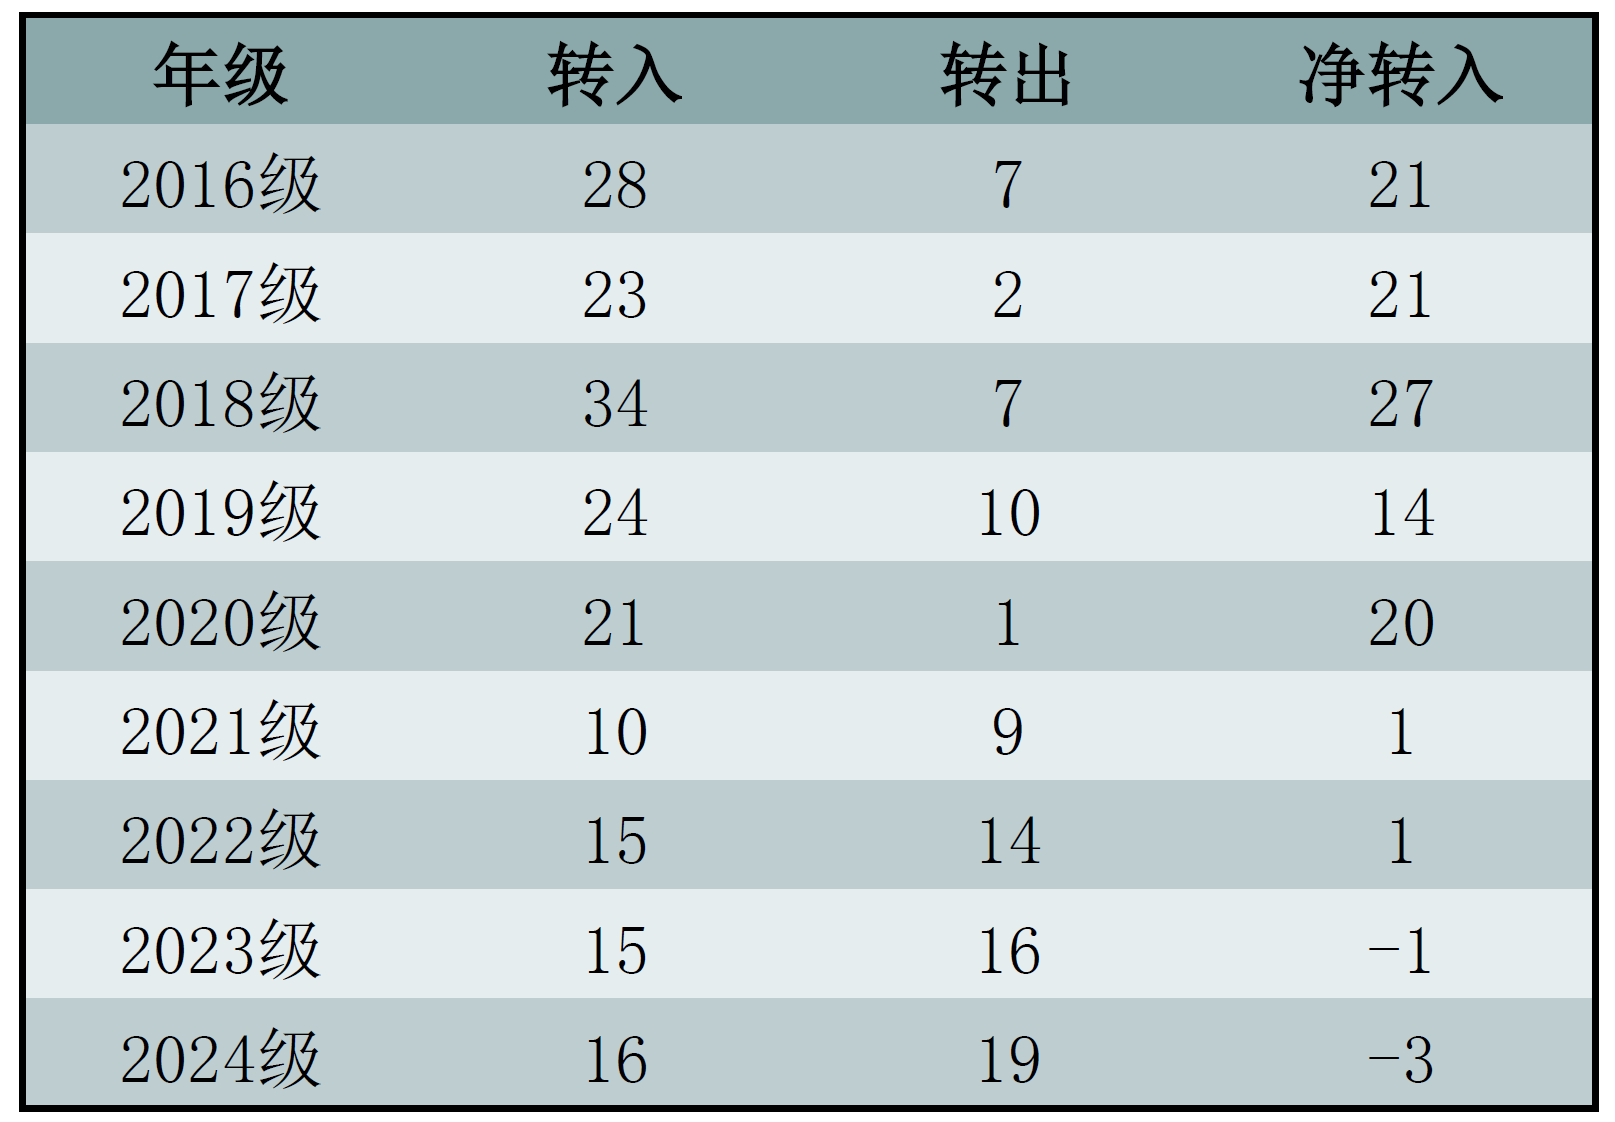
\includegraphics[width=0.6\linewidth]{assets/转入转出情况.png}
	\renewcommand{\figurename}{图}
	\caption{工学院本科生转入转出情况}
	\label{fig:enter-label}
\end{figure}

在这里，我们也为大家找到了几位智慧而热心的学长学姐，分享他们有关自己成功转专业的经历经验。

\subsection{工学院转出经验分享}
\subsubsection{（1）工院$\to$信科$\parallel$作者：一位希望保持匿名的同学，大一平转转入信科信息与计算科学专业（智班）}

\textbf{转院考量}：兴趣，以及对于未来的规划。建议入学后多了解各个方向，形成更全面的认识后再做决定。本人转信科并非因为觉得工院不好，而是心中向来对计算机抱有更大的热忱，报考北大时就已经坚定地向往去信科学习，只不过因为种种原因被调剂至工院。

\vspace{10pt}

\textbf{转院流程}：每年报名及考试时间不尽相同，请密切关注院系相关通知，或民间的转信科微信群。大概在每年三四月份，信科发布转院系通知后，按照要求填写和提交相关材料。之后教务会通过邮件通知考试时间和安排，按要求参加考试即可。

\vspace{10pt}

\textbf{课程规划}：仔细比对信科和工院（自己预期方向的）培养方案，做好转入信科和留在工院的两手准备。大一上的课大体相似，但是信科上计算概论A，工院上计算概论B（根据以往经验，如果计算概论B上80分，可以不用重新修读计算概论A）；工院上自己开设的数学分析和线性代数/高等代数，信科上数院开设的相应课程（根据以往经验，可以替代）。【以下仅针对部分计算机相关方向的专业，其他例如电子信息等专业会略有不同】大一下的课有部分差别。根据以往经验，普通物理Ⅰ可以替代专业选修课的物理类课程。信科多出来的两门专业课\footnote{程序设计实习和人工智能引论}需要在之后补修，可以选择这其中一门时间不冲突的专业课，减轻之后的补课压力。数据结构与算法B不可替代数据结构与算法A的，且数据结构与算法A是在秋季学期开课。

\vspace{10pt}

\textbf{考前准备}：多刷题，打好基础即可。转计算机相关专业的是机考（算法题），转电子信息相关专业的是笔试（物理）。民间转信科微信群里可能会有往年题，可以参考。面试中规中矩，不过也可以稍微准备一下。

\vspace{10pt}

\textbf{住宿调整}：一般不会换寝室。若确有需求，可自行找宿管申请。

\vspace{10pt}

\textbf{心态调整}：放平心态，即使没考过，大二还有机会，虽然届时课程规划会比较麻烦。实在没考过也不必太沮丧，工院也是非常值得留下来的。俗话说，三百六十行，行行出状元，真的用心学的话，在哪儿不都一样？

\subsubsection{（2）工院$\to$数院$\parallel$作者：原2022级\ 秦晟，大一降转转入数院数学与应用数学专业}
对于转院，我认为问题最大的可能不是报名流程，而是自己为什么要下这个决定。

\vspace{10pt}

1. 首先掂量的是自己想法的“纯度”和“目的性”。一定要避免一时脑子热、跟大流等类似情况。可以旁听几节课，并且注重自己在学这些课程的内心体验，看看是否真如自己所想。

\vspace{10pt}

2. 关于摇摆不定，我十分鼓励大家在遇到可能包括转院在内的各种疑惑时，多和老师、家人、同学沟通，之后再看看自己的想法是否有所松动。

\vspace{10pt}

3. 关于平转降转，仁者见仁，智者见智。一年的时间，可以看作节省，也可看作积淀。不同的选择有不同的注意事项：平转，提前选课；降转，较为灵活。

\vspace{10pt}

4. 关于流程，教务部每年都于四月中旬发布校本部转专业工作通知与各院系接收人数和考核计划，学生会也会组织转专业、双专业、辅修的交流会，有意向的同学可以关注北大教务部和校学生会公众号。

\vspace{10pt}

5. 关于重视程度，大家可能会将这类事情看得很重，认为大学专业关系到人生职业、未来发展，就犹豫不觉、不知所措。我想说的是，这么想百分之百没问题，但人生纷杂难测，机会众多，遵循当下自己的真实内心想法就好。

\vspace{10pt}

祝大家大学本科4（or 5 or 6）年快乐。

\subsection{转入工学院经验分享}

工学院的各位同学大概率用不到这部分内容，但是如果你身边有对转入工学院有兴趣的同学、朋友，可以把这些内容推荐给ta！

\subsubsection{（1）物院$\to$工院$\parallel$作者：2023级\ 李宗远，大一平转转入工学院机器人专业}

北大在大一下和大二下分别有一次转专业机会。我这届转专业在四月初开始报名，报名方式参考北大公示的文件。不过每年时间可能不一样，大家及时关注学院官网上发布的信息以及邮件。至于考核和接收时间就是各个学院自行决定了。我这届是在5月15日进行面试，大概一周后工学院公示转专业结果。

\vspace{10pt}

每年都北大会发布《XX年校本部各院系转院（系）转专业接收工作具体方案》，内含各个学院所接收的转专业人数、报名条件、报名方式以及考量方式等。在学院官网中可以找到以往的文件。2023和2024年工学院的报名条件都是“在校期间无不及格课程”，听往届学长说以前还对绩点有要求。

\vspace{10pt}

23年与24年工学院的转入考量都只有面试。我这届的面试流程是：学生先进行一分钟的自我介绍（随便说说就行，没多少影响），然后是老师提问。对我而言，老师问的问题是“你这学期选了多少学分的课”“你这学期选的专业课期中考试考了多少分”，然后提醒我要提高自己的绩点，我的面试就结束了（狗头）。我的面试时间属于很短的，我个人推测是因为我大一所修的课程和工院的培养方案基本吻合，并且我大一下的几门专业课的期中成绩都不错。

\vspace{10pt}

老师面试的主要目的是了解学生的情况，未必会问具体的专业问题。大多数老师也都很和善，现场的氛围倒是和茶话会挺像。和我一起参加面试另一位同学就被面试了五六分钟。他是一名大二的学生，想要降转工院。但他学习的数学课程是C级，而且在疫情期间选过pf，也退过课。我说的这三条都是面试过程中老师问他的点。

\vspace{10pt}

23年工院的招收人数是30人，最后公示接收人数是二十几人。24年工院的招收人数是40人，报名人数21人，接受人数16人，其中选择机器人工程的占了一半。在报名人数仅占接受人数一半的情况下，还是刷掉了五个人。个人推测，他们被刷掉的原因可能如下：课程选择与工院培养方案大相径庭或者成绩不好，工院老师担心他转入后跟不上课程进度；还有一种可能是选择转入机器人专业的人太多了，工院老师要考虑机器人系学生的保研竞争问题。

\vspace{10pt}

至于平转和降转，大家可以根据自己情况来选择，如果像我一样大一选的课和工院培养方案基本吻合，就可以选择平转，如果专业课有很大不同也可以选择降转，这样可以较好的跟上课程进度。如果课程相差很大还选择了平转，面试老师有可能会问你能不能跟上课程之类的问题。

\vspace{10pt}

如果以后工院的转专业考核还和24年一样的话，我的建议是在平时用功夫，多修些相关专业课，把成绩拉高，有什么问题及时询问工院的教务老师和有相关经验的学长学姐。也要记得去官网找最新的我在上文中提到的那几个文件——在大学里信息搜集能力十分重要。至于面试，没多少好准备的。当然，如果考核方式有所变化，就不要按照我的建议来啦。

\textbf{课程规划：}

在前文我也提到，我大一的课程选择与工院的培养方案基本吻合，这在一定程度上帮助我顺利通过工院的面试。因此，同学们可以去北大官网了解本科生培养方案（要找最新版的）。如果在大一上开始前或大一下开始前就决定转入工院的话，可以按照工院的培养方案进行选课，这样转过来以后就不用再补课了。或者选一些可以平替工院的课，比如B级及以上数学课。例如，工院23年的培养方案上写着，非强基生可以用高数B代替工院的数学分析。其实理学部学生大一的专业课有很多相似之处，比如高数，线代，普物，计概和数算，无非是不同专业难度不同。所以理学部的学生转入工院还是比较轻松的，如果是文科的同学想要转入工院，我建议提前修一些相关的专业课。

\vspace{10pt}

非工院学生要在选课的第三阶段才能选工院的专业课，不过工院大一的课程容纳人数很多，名额有很多空余，基本不用抢，在第三阶段选课也没什么影响。

\textbf{住宿调整：}

同学们在转完专业后，可自行选择留在原宿舍或申请换宿舍。留在原宿舍的好处是，和舍友已经很熟了，不用再磨合。如果和原宿舍同学相处得不太愉快，也可以借此机会换一个宿舍。新宿舍的同学有可能也是工院的，大家平时还可以一起交流讨论专业问题。转宿舍的具体流程，需和原学院以及工学院的学工老师沟通。

\textbf{心态调整：}

转入工院的难度要比热门的信科、数院小一些，考核也不多。因此，同学们不必焦虑，平时认真学习别挂科，在选课上多花些心思，提前去了解工院的几个专业，确定好自己的目标，转入工院就是水到渠成的事啦。

\vspace{10pt}

最后预祝想要转入工院的同学们都成功转进自己心仪的专业，欢迎你们加入工院这个温暖的大家庭！

\subsubsection{（2）生科$\to$工院$\parallel$作者：2022级\ 王喆楷，大一降转转入工学院工程与科学计算方向}
\textbf{\textbf{关于降转和平转}}\textbf{\textbf{：}}

平转即两专业学习无缝连接，降转则需要在新专业多读一年。

\vspace{10pt}

如果大家在转专业前后课程重复度较高，或者在转专业前所修的部分专业课，经过目标院系院教务认证，可以替代本院培养方案中的课程，个人认为可以直接选择平转。毕竟大一以通识教育为主，不同专业的培养方案大相径庭，有心预习目标院系的专业课的话，适应平转的压力并不大。

\vspace{10pt}

当然，也不必视降转为逃避。如果专业跨度较大，或者关键课程没有修读，完全可以投向降转。多余的一年时间可以更好地适应大学的模式，思考自己真正需要什么。担心荒废时间的话，可以在学有余力且确有热爱的情况下攻读一门双学位，或者提前联系导师进组。（P.S. 亲身体验，唯一的尴尬是说出自己的年级常常伴随着怀疑的目光……）

\textbf{住宿调整：}

转专业并不意味着会安排新宿舍。据我了解，除元培PPE和光华未来领导者等少数项目中，转入/申请者均搬入了对应的住宿，其他的转专业同学大多仍然维持着原宿舍。搬到同一寝室有助于专业课学习上的互帮互助，也能更快融入新学院。不过就我自己而言，选择了维持原宿舍，因同寝室内共三人转院，算上双学位便在一间寝室内凑出了六门专业，被朋友戏称小元培（bushi），在学术探讨方面为我提供了更多的跨学科体验。

\vspace{10pt}

住宿调整方面，可以直接前往宿管中心进行询问并申请调整，没有时间限制，随时有空位即可搬。值得一提的是，对于降转的同学，即便当前不换宿舍，在原定的毕业年份时（大三结束后）也需要搬出原宿舍另择宿舍。

\vspace{10pt}

\textbf{转院流程：}

1.询问往届学长学姐，善用搜索，了解往届院系互转的具体政策。我认为应该主要聚焦于一下信息：

·目标院系对转入专业有无限制/本院是否允许转出

·是否对降转/平转有特别要求

·是否需要某门课程必修 \& 该课程成绩要求

·对于成绩要求

·考核方式（面试/笔试）及可能涉及内容

\vspace{10pt}

在我转专业的那一届，信科仅限平转，设置上机考试且要求需修过计概A；物院转院考试，大一考察力学，大二涉及四大力学；数院则大一大二共用考卷……每年具体政策不同，以上仅为参考。建议尽量掌握当年的相关信息，以便规划自己的选课方案和时间管理。

\vspace{10pt}

2.北大教务网搜索转专业专区，下载附件，了解转专业申请时间线的大致的时间节点。

\vspace{10pt}

3.开放申请后，按照要求准备手续材料。

\vspace{10pt}

4.应对考核，静待结果。

\vspace{10pt}

最后，切莫把转专业当作治愈所有问题的良方。未来规划和学科适应程度确实改变了，可是你所遇到的问题却不会烟消云散，需要你自己去面对和解决。如果因种种原因未能如愿转系，也请放平心态，在北大自由的选课制度和双专业/辅修制度下，找到你的热爱。

\newpage

\section[双专业/辅修建议]{双专业/辅修建议\footnote{根据《北京大学2025年本科双专业申请审核工作通知》，2024年（含）以后入学的本科生按照《北京大学本科生修读双专业管理办法》执行。因此，对于大家而言，“双学位”已经是过去式。更多有关双专业、双学位、辅修的区分，详见3.5.4}}

\subsection{双专业/辅修简介}
北京大学鼓励学有余力的同学修读双专业、辅修专业，成为复合型人才。

\vspace{10pt}

修读双专业或辅修专业的部分考量列举如下：

（1）对某个非主修专业方向很感兴趣，有志于深入钻研的；

（2）认为某个非主修专业方向能够提升自己今后的能力、眼界、人脉、竞争力等的；

（3）希望以后直接转行至该行业的。注意：强基计划同学跨院系保研其他专业存在一定限制，请关注最新通知；

（4）希望所学辅双专业为主修专业赋能的。例如，信息学双学位可进一步提高代码能力，便于工科学业未来发展；

（5）暂时没有明确想法，但是学有余力，希望进一步丰富大学学术生活的。

\vspace{10pt}

当然，选修双专业或辅修专业的最大挑战是课业压力。例如，工院强基理力+经济学双学位的毕业要求约190学分\footnote{每年均会有所变动，请关注最新信息}。不过，学长学姐的经验告诉我们，时间就像海绵里的水，只要愿意挤一挤还是有的（bushi）。

\vspace{10pt}

关于双学位、辅修的常见核心问题，北大教务部网站有详细解答。具体路径：北京大学教务部官网——学生——双学位/辅修。双学位、辅修的详细培养方案也可通过上述路径获取。此外，学校或各院系会在春季学期初期举办转专业/辅双经验介绍讲座，有兴趣的同学可自行关注。

\vspace{10pt}

下面列出若干双专业/辅修的注意事项。笔者再次提醒大家，本手册任何有关现行政策的内容仅作参考，手册不保证绝对的准确性和时效性，请大家务必关注学校、各学院发布的最新通知。

\vspace{10pt}

（1）双专业需正式报名；辅修无需任何手续，直接选课、上课，并在毕业时向教务申请相应专业的学位认定即可。无法继续双专业学习时，可以申请退选双专业；若达到辅修毕业要求，也可在毕业时转为辅修。

\vspace{10pt}

（2）双专业课程通过专用通道进行选课，直接抽签决定而无需投点，每学期学分上限为30学分，根据该学期双专业课程学分总和收费\footnote{以国家发展研究院的经济学双专业为例，校内本科生学费为150元/学分，教学计划共42学分，总计6300元}。辅修课程通过普通选课“跨院系选课阶段”进行投点选课，每学期上限仍为25学分，不额外收费。

\vspace{10pt}

（3）双专业毕业要求学分多于辅修要求，具体数据大约是45：30，各院系各项目存在差异，主要体现在双专业要求的专业选修课会更多。

\vspace{10pt}

（4）某一门课程的学分只可认定一次。例如，国发院开设的经济学原理（3学分），既是通识课，也是经济学双专业的必修课。因此，在毕业时，该3学分或计入主修专业的通识课学分，或计入经济学双专业的必修学分，二者任选其一而不可兼得。

\vspace{10pt}

（5）毕业证书中标注双专业。例如，工学院力学类强基生选择了生物医学工程方向，则其毕业证上的专业标注为“理论与应用力学+生物医学工程辅修”；如果该同学还修读了国发院经济学双专业，则其毕业证书上或标注“生物医学工程辅修”，或标注“经济学双专业”。

\vspace{10pt}

（6）学位证书仅有一本。原有的双学位项目可获得两本学位证书，现行的双专业项目仅可获得一本学位证书，对于双专业授予辅修学士学位\footnote{注意：通过辅修是无法获得辅修学士学位的，所以虽然名为“辅修学士学位”，实则需要通过双专业获得}，辅修学士学位在主修学士学位证书中标注。

\vspace{10pt}

（7）重要时间节点：每年春季学期初，学校、各院系会开展转专业、双专业讲座，推荐大家关注。转专业、双专业的报名工作大约在4、5月开始，请大家关注学校、各院系的官网和公众号等信息渠道，亦多多关注自己的邮箱，防止漏失重要信息。

\vspace{10pt}

（8）双专业门槛：不同院系要求各异，但共同特点是门槛几乎为零，一般而言不挂科、成绩正常就行，且一般无需考试选拔。

\vspace{10pt}

（9）部分双专业/辅修与主修专业是互斥的，即特定的A、B专业不能同时作为主修和双专业/辅修。不过，工学院在这方面几乎没有受到限制。具体互斥信息请参见《北京大学辅修/双专业与主修专业互斥一览表》

\vspace{10pt}

（10）培养方案是不断更新的，且近几年也有新的辅修或双专业项目开设，请大家以最新文件为准。

\subsection{常见问题解答}
\textbf{（1）我到底应不应该修读双专业？}

浓厚长久的兴趣是修读双专业的关键。它能提供动力，有助于学好课程，在课堂内外主动获取更多相关知识。建议同学们在修读前，对培养方案、院系氛围、讲课内容进行一些了解，例如可以旁听课程，也可以咨询学长学姐。实在无法坚持学习，也可以选择退出。这并不丢人——大学是人生中试错成本最低的阶段，敢闯敢试才能让我们的青春不留遗憾。

\vspace{10pt}

事实上，笔者想强调的是，包括是否修读双专业在内的大学学习生活中的众多决策，功利因素的占比远没有大家想象的那么大，很多时候仅需问问自己：我真正感兴趣的是什么？跟着自己的内心走，才会有长久的动力。

\vspace{10pt}

\textbf{（2）学双专业有什么实际作用？}

实话实说，最大的作用不仅在于毕业证书和学位，更在于你在课堂上真正学到了什么，玄乎一点，是学习能力的提升和个人眼界的拓展，是对大学生活的一种充实和拓展。当然，双专业也对从事对应行业有一定程度上的帮助，至于程度大小：

\begin{figure}[htbp]
	\centering
	
\includegraphics[width=0.2\linewidth]{assets/2.1.1衡量.png}
\end{figure}

\vspace{10pt}

\textbf{（3）修双学位要提前准备什么吗？}

无需刻意准备，先把主专业学好了再说。兴趣十分浓厚的同学可自行阅读相关专业书籍。

\subsection{学长学姐经验分享}
\textbf{国家发展研究院-经济学双学位$\parallel$作者：2020级\ 瞿朱毅}

经济学双学位由北京大学国家发展研究院开设，据往年经验，一般要修42学分左右，包含必修课：经济学原理、中级微观经济学、中级宏观经济学、计量经济学和中国经济专题，以及其他选修课。在各个双学位课程中，经济学双学位相对轻松，录取也较为容易。想要未来从事经济学学术科研的同学可以选择相应课程，如做微观理论的可以选学产业组织、博弈论等，如想转商科金融的建议尽早修完财务会计和财务报表分析等。

\vspace{10pt}

我当初选学经济学双学位是怀着跑路的心态去的，就是想通过修经济学双学位研究生转往经济学方向，但后来发现经济学学术科研内部内卷严重，工院给分一般导致研究生转到经济学较为困难，故放弃该想法，就把经济学纯当一个兴趣和“白月光“式的存在了。后来强基计划保研政策也公布了禁止转入经管。

\vspace{10pt}

感觉我最后还是有一些收获，譬如做了助教挣了钱，找到了女朋友（笑），也学会了用经济学的视角分析问题。当然也有遗憾啦，遗憾就是大一没有选上双学位导致有一些必修课放到了紧张的大三去修。优势就是能够多拿一个学位（笑），多认识一些人，多获得一些知识，以及提升绩点，劣势就是在大四还有一堆课，挤占了科研时间。如果说有啥建议的话，那我该说，去努力发掘自己的爱好是一件重要的事情，有些时候经双修的好能够给你从工院低分的挫折里找回信心。

\section{学业导师}

\subsection{简介}

工学院会为每位新生统一安排一位学业导师，请大家关注教务老师的通知。根据笔者经历，每位导师负责3至4位同学。每学期，大家需要和学业导师至少完成3次面谈交流，并填写指导记录，在每学期的期末周前上交至院系教务处。

\vspace{10pt}

学业导师主要关注同学的大学生活适应、选课上课、专业方向选择、个人学习计划制定、职业生涯规划等，会在力所能及的范围内，给予大家真诚的建议。鉴于许多学业导师都有自己的课题组，所以除了课业与生活，大家也可向自己的学业导师了解行业学界前沿和导师研究方向，亦可在他们的指导帮助下参观实验室、阅读相关论文等，增进自己的综合学术能力。

\subsection{一些补充}

（1）部分同学可能囿于性格内向，不愿或不敢与学业导师交流太多。事实上，大家无需紧张担心，在最为基础的礼貌之外，许多老师都是十分随和的，大家把老师们当作是一位朋友即可。不必担心“我说了这句话，老师可能会对我产生什么看法”，也无需害怕“我的这个观点和老师的不一致，会遭到强烈反对”。大学之大在于有容乃大，大家在不打破基本原则、不违反公序良俗的前提下，尽情表达自己的真实想法，相信老师一定会给予尊重和真诚的指导。

\vspace{10pt}

（2）大家在每次面谈交流结束后，需填写指导记录并交由导师签字。指导记录表可在学院教务办公室直接领取纸质版，亦可从工学院官网下载打印。

\vspace{10pt}

（3）建议大家在学期初规划面谈大致时间，例如第1、8、16周。我们推荐大家参考开学、期中考试、期末考试这三个时间点，以期与学业导师的交流带来更多收获。或许老师考前的某一句复习指导就点通了你的任督二脉呢？

\vspace{10pt}

（4）提前发送邮件，与学业导师预约具体时间。正式的格式、有礼的称呼和礼貌的问候总不会出错。建议在预约时间前5分钟左右到达\footnote{视情况而定，并非墨守成规}，这一小段时间体现的，是你对学业导师的尊重和对面谈交流的重视。

\vspace{10pt}

（5）对每次交流予以足够重视。老师们学术科研经历丰富，研究方向各异，他们的分享和指导对我们的学习方法、未来方向、生涯规划甚至价值观念，都会有一定程度的影响。因此，我们应该充分利用好学院给予我们的宝贵资源，在话语之间力求自我提升。切忌把面谈看作是被迫完成的任务，那会使指导效果大打折扣，且会令你在未来的某个时刻后悔，为何当初没有好好珍惜交流机会。

\chapter{学工社团}
\section{学工简介}
大学生活的一个重要组成部分就是学生工作。

\vspace{10pt}

区别于中学，在大学中做学生工作的同学们有更多可以调动的资源，当然这也就意味着更大的责任。如果说“努力学习”是在学术方向上的努力，那么学生工作就是在社会方向上的探索。它教会你怎么服务更广大的群体，怎样和人打交道，怎样做出让大家都满意的工作，所以学生工作是服务他人的方式，更是锻炼自己的机会。

\vspace{10pt}

学生工作范畴极大，大体工作领域可以分为：班级、院学生会、院团委、校学生会、校团委、学校各级工作单位。

\vspace{10pt}

班级干部工作，主要负责上传下达，跟中学类似，不做赘述。

\vspace{10pt}

接下来简要介绍院级单位和校级单位工作区别。在院级单位，无论是学生会还是团委，我们的工作绝大多数都是围绕学院的师生展开的。优势是我们可以和同院师生更加亲近，能收获更好的关怀；劣势是很少走出学院的“一亩三分地”，活动规模相对较小。在校学生会和校团委的工作则面向全校师生展开，可以结识各个学院的同学老师，参与组织学校的大规模活动，但是可能和学院的同学相对比较生疏。

\vspace{10pt}

学生会和团委（院、校同理）的区别，是很多同学都会有的困惑。简要介绍如下：团委举办的活动相对更加正式，强调思政引领；工作模式和风格相对更加规范，组织严明。学生会是党政机关和广大学生联络的纽带，其工作内容和团委有一定程度的交叉，组织架构和团委也较为类似，但是举办的活动相对轻松，工作模式和风格相对自由。

\vspace{10pt}

是院团委、院会，还是校团委、校会，如何选择需要同学们自行衡量。

\vspace{10pt}

最后我们来说学校各级工作单位的学生助理。很多单位都招收学生助理，例如学生工作办公室助理，招生办公室助理……这些工作的工作时间固定，需要跟老师协调；工作内容是协助老师完成日常工作，对于了解该单位的工作以及相关领域的动向有一定帮助；另外值得一提的是，这些工作有固定的薪资酬劳。工作的招募一般在该单位的公众号上发布，有意的同学可以密切关注公众号。

\vspace{10pt}

同学们还可以通过辅导员老师，或者通过学院官网coe.pku.edu.cn——教职员工——行政人员，联系各位老师解决学生工作方面的问题。

\section{学工组织}

有关校学生会、校团委，上面已经有过一些介绍。详情请关注公众号“北京大学学生会”和“北大团委”，在这里不做赘述。下面详细介绍工学院学生会和团委的情况。

\vspace{10pt}

\subsection{工学院团委}

在工学院团委这个温馨的大家庭里，你可以收获：

\begin{itemize}
    \item 深度参与学院大型活动组织策划的体验。
    
    \item 更早获悉学院一手信息的机会。
    
    \item 较为专业的办公技能锻炼以及组织能力磨炼的机会。
    
    \item 丰富的阅历和视野，同时通过社会实践/志愿服务团体（例如组织参加支教等志愿服务活动）增长社会技能。
    
    \item 有优秀的学长学姐耐心引路，与志同道合的朋友共同进步的机会。
\end{itemize}

\vspace{10pt}

学院团委主要包含办公室、组织部、宣传部、实践部、社团运营中心、文体部、体育发展中心、青年志愿者协会、周培源宣讲团等部门，招新时间待定，招新对象为工学院全体同学。详细介绍请参考公众号“工映青春”上的招新推送。去年的推送为2024.9.11《招新｜工学院团委部门招新啦！》，敬请期待今年的招新推送。

\vspace{10pt}

补充：学生工作不是所有同学一定要参加的。事实上，北大任何活动几乎都没有强制性。但参加学生工作，不管是在功利角度还是非功利角度，都会有莫大的收获。请同学们根据自身实际情况，尽力而为，量力而行。

\vspace{10pt}


\subsection{工学院学生会}

学生会是联系学校、联系广大同学的桥梁和纽带。工学院学生会的宗旨是服务同学、虽小却精、氛围融洽、活动自主。

\vspace{10pt}

在这里你能体验到：

\begin{itemize}
    \item 有趣而温暖的文化。学生会以友爱为先，工作氛围极好，工作压力较小，没有恶性竞争，能获得很强的归属感。
    
    \item 丰富而自主的活动。不仅可以体验到各种活动，更可以提供你的点子，为学生会和学院同学创办一些新的活动方案。相对而言，团委的工作更偏向于正规和纪律性，请大家选择自己合适的工作风格。
    
    \item 满满当当的成就感。活动能锻炼同学们的能力和眼界，在学生会自主性质的加持下，更能让同学们体会到成功举办活动带来的满满当当的成就感和自我实现感。例如，本手册就是完全由工院学生会学术实践部自主发起和编写的，在撰写的过程中编者也感受到了自我价值的实现！
    
    \item 优秀而贴心的学长学姐。学生会的学长学姐不仅本身优秀，更是极其愿意帮助低年级的同学们成长向上，在这里你会收获很多生涯发展方面的启发。
    
    \item 志同道合的同学。如果你急于解决5.3.2小节中提到的问题（4）“社恐，想社交但实在不会、不敢，怎么办？”，亦或者你在认为自己的满腔热血和抱负需要寻找伙伴一起实现，那么学生会各部门一定能为你提供这么志同道合的一批人，助你实现自己的理想。
\end{itemize}

\vspace{10pt}

学生会现有办公室、外联部、内联部、文体部、宣传部、学术实践部六个职能部门，预计在新生军训、新生训练营期间进行招新，招新对象为工学院全体大一、大二同学。详细介绍请参考公众号“工映青春”上的招新推送。去年的推送为2024.8.21《工学·招募｜工学院学生会招新开始啦！》，敬请期待今年的招新推送。

\vspace{10pt}

随着新工科时代的到来，工学院以及工院学生会的影响力正越来越大，诚挚欢迎大家加入工学院学生会，共创我们的工学新天地！

\vspace{10pt}


\subsection{党建工作委员会}

工学院党建工作委员会为中共北京大学工学院委员会下属工作机构，直接负责基层党组织各类事务，引领党员坚定理想信念，吸纳更多优秀人才加入党组织。二十大以来，构建新时代“系统党建”，充分发挥党员先锋模范作用、基层党组织战斗堡垒作用、人民群众参与作用，是提高党的建设质量的必然选择。党建工作委员会作为党的建设力量的火车头，每一名成员都能够在这里获得思想的淬炼、政治的历练和能力的锻炼。党建工作委员会下设组织部、学习部和综合办公室。

\vspace{10pt}


\subsection{班级建设工作委员会}

工学院班级建设工作委员会是工学院下属工作机构，负责班级各类事务及班主任、辅导员、班委队伍组织建设，旨在夯实工学院基层班级组织建设，引导班级在同学中发挥更大影响力与号召力，加强班主任、带班辅导员、及青年委员等班委队伍凝聚力，提升班级文化建设活动质量。

\section{社团简介}
每学期开学的第二或第三周周末，在百讲与新太阳区域会举行“百团大战”。届时会有上百个社团在场招新，并且在摊位上举办各自的特色小活动。如有兴趣，可以积极参加百团大战并添加相应社团公众号/微信群进行了解。

\vspace{10pt}

社团的一些特点是：

1. 自治性很强，其活动在团委指导下由学生自行组织。

2. 对外开放性不大，导致很多社团甚至不为人所知，看似自娱自乐，实则社员中卧虎藏龙，社团内到底在研发什么“秘密武器”，外人啥也不知道。

3. 加入社团没有任何硬性条件考核，完全出于兴趣，很好地体现了北大“思想自由，兼容并包”的精神。

4. 在社团里好好干还是划水、参加还是不参加活动，完全不受强制，完全出于个人意愿，十分自由。因此一般不会大量占用学习时间导致成绩下滑。

5. 不同社团大小、氛围差异很明显。

6. 社团中也会有负责人等，这也是一种学生工作。

\vspace{10pt}

因此，加不加社团，加几个社团，也是一件“需要你自己衡量”的事。

\section{入党相关}
加入中国共产党是一件极为严肃的事情。同学们应当在坚定信念后再选择入党，而不是人云亦云，“跟风”入党。

\vspace{10pt}

入党有以下几个流程：提交申请书——入党积极分子——发展对象——预备党员——正式党员。以上每次身份的转变都需要经过学习、行动与考察，且周期比较长（总计至少两年多）。

\vspace{10pt}

由于流程很长且较为繁琐，这里不赘述。如果读者有志入党，随时可以提交入党申请书给党支部。注意，入党申请书不必等人统一收取，这是很多人的误区；一般来说给班级辅导员也可以，由其转交。提交申请书后，后续所有流程都会接到通知。

\vspace{10pt}

另外提醒：要牢牢记住重要时间点，如何时入团/党，何日提交申请书，何日被推荐为积极分子等等，这会为以后填写资料节省很多时间。

\section{其他学生组织与课外活动}
\subsection{志愿服务}

志愿服务是提升人奉献精神和工作能力的良好契机。同时，一定的志愿时长\footnote{在“志愿北京”小程序或网站可查看具体时长}还能给综测带来加分，从而给评优评先带来一定优势。因此，花费适当课余时间在志愿服务上，无论从功利还是非功利的角度，都是非常值得的。当然，我们也不鼓励大家去卷过多的志愿时长\footnote{注意综测加分48小时封顶}，重心仍然应该放在课业学习中。

\vspace{10pt}

首先，需要在志愿北京官网 https://www.bv2008.cn/ 上注册账号，并自行记住用户名、密码、志愿者编号等信息。以后在你参加志愿活动后，组织方一般会要求提供志愿者编号，并为你录入相应时长或下发纸质证）。

\vspace{10pt}

有的同学苦恼于志愿时长无处可觅。因此，下面介绍几个重要的志愿服务渠道。具体的信息收集仍需要同学们自力更生。
\begin{itemize}
	\item 校级活动：五四青春长跑志愿者、北京大学图书馆志愿者、返乡宣讲、学生会/团委/青协等学生组织的活动。
	\item 院级活动：较为零散，但是有活动必有志愿服务需求。有意向的同学请咨询学工老师或学长学姐以进入工学院志愿者招募群。
\end{itemize}

\subsection{学校活动}
学校活动数不胜数，种类繁多，只要你想得到，一般就能找得到。

\vspace{10pt}

学校层面，除了基本的学工、社团之外，还有百周年纪念讲堂的演出\footnote{详见百周年纪念讲堂公众号}、佳节时分\footnote{中秋、跨年等}的歌会、十佳歌手大赛、十佳主持人大赛、各种球类的新生杯/北大杯、餐饮中心的厨艺大赛、图书馆的讲座、地方支教等等各种形式的活动，且每个都能带给你别样的体验。活动报名信息获取渠道极为广泛，有意愿的同学请务必时刻关注相关公众号，善用搜索，善于向身边人提问。

\vspace{10pt}

学院层面，值得参与的活动也很多。例如由学生会承办的迎新晚会、保研出国经验分享会等；院友之声系列、学生心理类系列等讲座，在此列举不尽。主要关注的信息渠道有：公众号（见手册7.2.1节）、年级群、班级群等。

\vspace{10pt}

眼观六路，耳听八方，积极获取信息，相信你一定能找到自己热爱的舞台！

\subsection{一则鼓励}
如果你有好的想法，可以向上级建议或自行创办有积极意义的学生组织！

\chapter{积极心态}
相信大家既然历经重重考验来到了北京大学工学院，心理素质都是极强的，每个人都有不同的办法调节心情心态。在军训及新生训练营期间，同学们也会接触到一系列心理讲座，让大家对北大的学习和生活建立良好的心态。在这里，我们针对性地列出一些工学院学生常见的烦恼，并提供一些建议，希望能帮助同学们做好基本心理建设，以积极向上的姿态投入到学习和生活之中。当然，建设强大的内心本就是一个见仁见智的过程，我们希望大家能够吸取其中对自己有用的建议，大胆摒弃行之无效的方法，走自己的道路，过自己的美好人生！

\section{新生面临的核心问题}
这是一个很宽泛同时又很重要的话题，笔者不敢妄下结论，抛砖引玉，供管中窥豹。

\vspace{10pt}

大学生活与高中生活的不同，要从日常生活和工作两方面说起。

\vspace{10pt}

在日常生活方面，大学可能是很多同学第一次长时间离开家，随另一个群体生活。与高中生活不同的是，我们得不到高中那样不请自来的关注和指导，因此绝大多数事情需要我们自己去问、自己去摸索，而不能依赖别人主动地悉数灌输给我们。这时候，\textbf{独立性}和\textbf{主动性}就显得格外重要。我们需要学会自己探索，主动求教，为自己的生活负责，这样才可以克服生活中遇到的种种难题。

\vspace{10pt}

此外，我们需要面临更真切、更近距离的来自人际关系方面的压力。室友，同学，辅导员，老师……处理人际关系的责任不容推脱地落在了我们身上。而由于不同的文化环境、性格、目标等因素，孤独、矛盾等是不可避免的。笔者想说：人际关系最终的处理水平，仍然取决于我们的主观选择。如果他人没有恶意，宽容和体谅总不会出错。

\vspace{10pt}

可能有同学已经注意到笔者分类模式是日常生活和“工作”而非“学习”，这是因为人各有志，一些同学不将学术作为未来人生的总目标，这是完全可以理解的。因此我们广义地讲“工作”。

\vspace{10pt}

在工作方面，同学们会感觉到前所未有的自由，因为没有人会实时紧盯你的状态，工作和娱乐的权利全在你的手上。如果说高中是轨道，那么大学便是旷野；高中是一幅不容一点瑕疵的工笔画，那么大学便是一张一尘不染的白纸。白纸意味着没有上限，当然也没有下限；这句的前半句是激励，后半句是警告。没有人会阻止我们过放浪形骸的生活，当然也没有人会为我们设定天花板。北大便是这样，资源就摆在那里，不会主动喂到你的嘴边；但是只要你愿意争取，那学校便毫不吝啬地把资源向你倾斜。也许，一些同学已经对“自律”一词有了过犹不及的嫌恶，但是这里笔者仍然将\textbf{“自律”}作为一条极其重要的建议。当然，我们不鼓励打鸡血式地内卷，而是希望同学们想清楚自己想要什么、想成为什么样的人，并实时审视自己是离目标越来越近还是渐行渐远。如果适量的惬意休息是海船暂时归港，那么不易察觉的长期放纵便是摧毁海船的暗流与漩涡。

\vspace{10pt}

总之，建议有三：一是为自己负责，二是独立与主动，三是宽容与体谅。笔者真诚的期待同学们可以迎来四年无怨无悔的大学生活。

\section{如何利用好资源寻求心理帮助}
学校为我们开设了完备的心理服务。心理咨询中心会开设各类主题活动，可以关注公众号“北大学生心理健康教育与咨询中心”以参加相应活动。如果遇到难以解决的困难，可以拨打心理咨询中心电话：前台62760852 ；24小时心理援助热线62760521。

\vspace{10pt}

我们应该始终记得：心理障碍或创伤，和肉体上的创伤是一样的，是不可抗因素，不显示主观意志的强弱。当我们觉得难以支撑、心力交瘁时，要知道，这不是因为我们脆弱或敏感。因此，请积极地向外界寻求帮助，这并不羞耻。相信心理障碍可以被克服，我们终究会迎来拨云见日之时。

\section{常见问题荟萃}

说明：本部分内容仍待拓展，欢迎大家在我们的问卷中留言或投稿，也可以向我们私发消息。我们会选取具有普遍性的问题进行研究和约稿后写入手册（问卷二维码见手册“后记”）。

\subsection{学术类}
\textbf{（1）没有竞赛基础怎么适应工学院的学习生活？}

相对其他学院，工学院的竞赛基础没有那么夸张，请大家放心“祛魅”。且工学院相对更重视计算而非技巧，因此不必因为无竞赛背景而感到压力。此外，大学课程的重点与高中竞赛并非完全重合，有竞赛基础的同学也不能过于掉以轻心。

\vspace{10pt}

\textbf{（2）选了数院/物院/信科的课程成绩很差怎么办？}

首先，我们要承认其他人在天赋和基础上的优势，再看自己是否能够在意志品质上找补。如果发现成绩不尽如人意，那么建议综合权衡得分和难度，再进行选择。诚然，数院物院的课程相对难度更大，抽象程度更高，但不见得就不适合工学院同学进行学习\footnote{毕竟力学系学生拿过数学系数分第一名的传说不是盖的}，具体如何选择需要同学们自己衡量。

\vspace{10pt}

另外，在一门课程中取得不理想的绩点，并不意味着“天塌了”。一门专业课的成绩不佳也不能说明你的学习能力不如他人。或许是由于对课程难度的预估不准，或许是由于某次的考试失利。这一次失利放在整个大学上百学分的课程的学习之中也不过沧海一粟。同学们不必对自己过分苛刻，调整心态，再接再厉即可。

\vspace{10pt}

\textbf{（3）身边人都开始卷绩点/科研，我怎么办？}

生活不是竞技场。看别人干什么就跟风干什么，最终一定是内卷到疲惫且痛苦的。大学并非单行道，“3.92”\footnote{指绩点，是一个树洞里的梗}也不是所有问题的通解。因此，我们最好在一开始就做好大概预期，未来是做学生工作，还是搞科研，是留在国内还是去国外，然后再决定自己的生活节奏。不要人云亦云，做无意义的焦虑。

\vspace{10pt}

当然，也不建议因为没想好上述事情而焦虑，关于前途的考量，很多人是大三大四才定下来的，此所谓“车到山前必有路，船到桥头自然直”的智慧。笔者认为，大一最主要的任务无非就两件事：适应大学节奏、打好专业基础。真正做好这两件事就很好了。

\vspace{10pt}

至于科研，大一的同学更不必过早的焦虑，学好专业基础课后，再慢慢了解各个课题组，发掘自己的感兴趣的方向即可，“为了科研而科研”是行不通的。（夹带私货：有强烈的意愿的同学也可以关注院学生会举办的本研动力学讲座~）

\textbf{（4）面对大一末的分流，我应该做什么准备？}

在大一期间，同学们可以通过多种方式了解工学院的各个方向。大一上的现代工学通论课程，大一下的“工学嘉年华”活动、“工学文化节”，以及在分流前的专业介绍讲座，都为同学们提供了多样的了解工学院不同专业的方式。分流截止至大一结束的暑假初期，在大一下期末会进行一次预选以及召开一次针对预选结果的年级大会。大家也可以多与不同方向的学长学姐沟通交流，充分了解后进行选择。

\subsection{生活类}
\textbf{（1）除了做题，感觉自己其他啥也不会怎么办？}

\vspace{10pt}

工学院某位著名的“人生导师”曾经说过：“在北大，千万不要把自己太当回事，也千万不要把自己不当回事；千万不要把别人太当回事，也千万不要把别人不当回事。”无论是感觉自己“啥也不会”，还是感觉别人“啥都会”，事实上都是太把别人当回事，却把自己不当回事了。事实上，北大将教会你的第一件事情就是“祛魅”。让身边许许多多人不再被“神化”，许许多多事情不再“遥不可及”，大家都有自己的优点和缺点，很多也都是经历了高中的“小镇做题”阶段才进入北大的\footnote{必须承认的是，会做题本身也是很大的优点}。大家都是一张白纸，等待着自己花四年甚至更多时间，书写在北大的精彩人生。

\vspace{10pt}

北大会让你认识到的第二件事情，就是有梦想就会有实现的机会。第4章已经说了，只要想得到的活动一般都能找得到。在北大，资源不会主动找上门。但如果你积极地去找，一般都能找到很好的资源进行学习，同时试错的成本极低\footnote{花钱少，不用找关系，地理位置近，教学内容专精……}。因此，即便你现在觉得自己“啥也不会”，等过了一个学期、一年、四年，你会发现自己冥冥之中有了巨大的提升。

\vspace{10pt}

第三，数院有人说过：“来北大我可能没有成为最好的那个，但至少我知道了最好的是什么样子。”即便发现自己有些事情努力了也做不成，但是你已经去尝试过，也见过最好的事物是怎么样的，这本身就是一个眼界和能力的巨大提升，对未来帮助很大。同时，在未来你仍然有机会再次挑战它。记住，你才18岁。

\vspace{10pt}

\textbf{（2）学工、活动占据过多时间，导致成绩下降怎么办？}

\vspace{10pt}

工学院的一位著名学长曾经说过：“大学就是在不同赛道上成就自我。”大学赛道不再单一化，成绩不再是成功的唯一衡量标准。在成绩基本盘hold住的情况下\footnote{指至少不能挂科，成绩还说得过去}，有的同学选择深入钻研课程，力争更高的成绩，为将来保研出国和深入研究打下基础；有的同学选择将大部分时间投身科研，追求知识的深度，早早开始挑战真正有希望为人类世界带来GDP的业界技术难题；有的同学选择学习辅双或选择其他院系的课程，拓展自己的学术兴趣、志趣，在知识的广度上实现自我价值；有的同学选择投入学工，发挥自己的社交属性，和老师、同学们深入交流，并在工作中锤炼实用技能，为将来的工作能力奠基；有的同学不断寻找实习，为将来进入业界打下坚实的经验基础，同时凭着实习的工资实现小小的“财务自由”；有的同学选择多多参与文体活动，在活动中绽放自我，结交朋友，成为舞台上最闪亮的星星；有的人拓展自己的爱好，坚持养成一个个好习惯，不在外表上宣扬自己的强大，内核却永远在悄悄变强，期待着惊艳大家的那一天……以上种种，都是“赛道思维”很好的体现。只要是实现了自己的价值就有意义，不能说哪条赛道就一定比另一条好，正所谓“不管黑猫白猫，能抓到老鼠的就是好猫。”

\vspace{10pt}

因此，如果出现了上述类似的问题，笔者的建议是：你需要衡量自己心目中各条赛道的优先级，坚守课业成绩基本盘不动摇的同时，摒弃“成绩为王”的高中生思维定势，选择最能实现自我的道路坚定地发展。

\vspace{10pt}

\textbf{（3）和家长、同学、恋人关系出现危机，影响正常生活，怎么调整心情？}

\begin{itemize}
	\item 直面并解决问题。建议直接当面或电话沟通，线上聊天往往可能引起歧义。
	\item 吐槽。跟信得过的老师、好友吐槽。大学新增的方法是树洞吐槽。
	\item 把事情扔一边先冷静。如果不是很急于解决，先不管这件事情，正常学习生活一段时间，冷静之后再回想。
	\item 咨询。当影响很大时，千万不要藏着掖着，要敢于寻求专业的心理援助。事实上，心理咨询中心不能看作是“治病”的地方，更多时候它是一个可以放心跟人吐槽，同时有人帮你理性分析、解决问题的地方。
\end{itemize}

\textbf{（4）社恐，想社交但实在不会、不敢，怎么办？}

社交是大学的必修课。首先，不要用标签框定自己（如MBTI），要知道社交属性到大学是会变化的（例如有的同学由i转e）。其次，不同性格的人各有舒适区，具体不再赘述，请大家自行感受，并学会悦纳自我。最后，还要意识到一件事情是，社恐和社牛并没有明显的界限划分，大多数人其实是处于中间的灰色地带的。

\vspace{10pt}

认识到以上几点之后，相信“社恐”的同学就不会再过多产生社交焦虑了。如果实在觉得自己需要社交的机会，不妨先从大胆参加活动、多多认识志同道合的朋友开始吧。当然，最终能不能成为朋友很多时候是看缘分，强求不来。

\vspace{10pt}

最后提醒大家社交把握尺度，拥有自己的判断力，不要让盲目社交影响了你健康的生活和正常的自我发展。

\chapter{大一时间线概览}

在大学生活这款开放式沙盒游戏里，我们总会在各种时间阶段遇到各种“事件”。本章试图将第一年的“事件”连缀成章，绘制大一生活的一张草图，帮助大家更快速地适应、更从容地规划丰富多彩的校园生活。也正因北大的生活过于多彩、选择过于多元，本章一定是平平无奇、挂一漏万的。因此，本章不是大一年级的“通关攻略”，而更应视作一张标注了NPC大致位置的参考地图。

\vspace{10pt}

此外，本章会加入大量索引，链接到前文内容。因此，也可以在茫茫信息涌到面前时，将本章作为一个大型、成文的目录，以便按需阅读全书内容。

\section{第一学期（秋季学期·开学前）}

\vspace{10pt}

\begin{center}
\begin{tikzpicture}[yscale=1.0, transform shape]
    \draw[chapc, line width=2pt] (0,0.35) -- (0,-13.55);

    % --- 1~4: 2倍间距 (4.4cm) ---

    % --- 1 ---
    \fill[chaph] (0,0) circle (4.5pt);
    \node[anchor=east, font=\small\bfseries, text=chapb, text width=3cm, align=right] at (-0.5,0) {8月下旬--9月上旬};
    \node[anchor=west, text width=11.3cm] at (0.5,0) {\textbf{英语分级考试}\\[2pt]{\footnotesize\color{chapc} 测试一般发生在军训后、开学前，题型涉及听力选择、阅读理解、词汇、语法、完形填空等，都是选择题，判卷速度很快(x)。正如3.3.4节所述，大家以最自然的状态参与分级测试就是最好的，适合的才是最好的。当然，如果你希望争取免修，或感觉直接去考反映不出自己真实水平，或就是莫名地不放心，可以找来各类英语考试的题目做一做。然而，笔者认为，为此刷题是不值当甚至不理性的。}};

    % --- 2 ---
    \fill[chaph] (0,-4.4) circle (4.5pt);
    \node[anchor=east, font=\small\bfseries, text=chapb, text width=3cm, align=right] at (-0.5,-4.4) {9月上旬};
    \node[anchor=west, text width=11.3cm] at (0.5,-4.4) {\textbf{新生训练营、新生定向越野}\\[2pt]{\footnotesize\color{chapc} 新生训练营帮助大家熟悉校园，做一些破冰活动，同时会有开学第一跑，可能会有神秘嘉宾哦！在定向越野中，你将和宿舍的同学一起在园内四处奔跑，完成一些有趣的游戏，继续熟悉校园。}};

    % --- 3 ---
    \fill[chaph] (0,-8.8) circle (4.5pt);
    \node[anchor=east, font=\small\bfseries, text=chapb, text width=3cm, align=right] at (-0.5,-8.8) {开学前};
    \node[anchor=west, text width=11.3cm] at (0.5,-8.8) {\textbf{选课}\\[2pt]{\footnotesize\color{chapc} 选课是门大学问，信息浩如烟海。详见2.3-2.5，也建议大家善用搜索。}};

    % --- 4 ---
    \fill[chaph] (0,-13.2) circle (4.5pt);
    \node[anchor=east, font=\small\bfseries, text=chapb, text width=3cm, align=right] at (-0.5,-13.2) {第1、2周};
    \node[anchor=west, text width=11.3cm] at (0.5,-13.2) {\textbf{第一次学业导师交流}\\[2pt]{\footnotesize\color{chapc} 笔者建议大家珍视同学业导师的每一次谈话。可以尝试在日常记录下自己遇到的、或大或小的困惑与问题，整合起来便于提问。当然，学业导师多由青年教师担任，因此大家不必焦虑，更不必以为学业导师全知全能，只要自然、愉快地开展沟通就好。详见3.6节}};


\end{tikzpicture}
\end{center}

\section{第一学期（秋季学期·期中前）}

\vspace{10pt}

\begin{center}
\begin{tikzpicture}[yscale=1.0, transform shape]
    \draw[chapc, line width=2pt] (0,0.35) -- (0,-16.85);

    % --- 5~8: 1.5倍间距 (3.3cm) ---

    % --- 5 ---
    \fill[chaph] (0,0) circle (4.5pt);
    \node[anchor=east, font=\small\bfseries, text=chapb, text width=3cm, align=right] at (-0.5,0) {第1、2周};
    \node[anchor=west, text width=11.3cm] at (0.5,0) {\textbf{工学院图书漂流活动}\\[2pt]{\footnotesize\color{chapc} 一般会在开学后的某个周末举行，让大家获取学长学姐的教材和参考书，节约购书成本。}};

    % --- 6 ---
    \fill[chaph] (0,-3.3) circle (4.5pt);
    \node[anchor=east, font=\small\bfseries, text=chapb, text width=3cm, align=right] at (-0.5,-3.3) {约第二周周末};
    \node[anchor=west, text width=11.3cm] at (0.5,-3.3) {\textbf{``百团大战''社团招新}\\[2pt]{\footnotesize\color{chapc} 上百社团同时招新，所以叫"百团大战"，在新太阳学生中心与百讲区域举办，是体验社团（整活）文化的绝佳机会，见4.3节。}};

    % --- 7 ---
    \fill[chaph] (0,-6.6) circle (4.5pt);
    \node[anchor=east, font=\small\bfseries, text=chapb, text width=3cm, align=right] at (-0.5,-6.6) {9月下旬};
    \node[anchor=west, text width=11.3cm] at (0.5,-6.6) {\textbf{秋季运动会}\\[2pt]{\footnotesize\color{chapc} 北大在春夏秋冬都会举办运动会，侧重的项目有所不同，其中秋季运动会也是新生趣味运动会。感兴趣的同学可以实时关注相关公众号。}};

    % --- 8 ---
    \fill[chaph] (0,-9.9) circle (4.5pt);
    \node[anchor=east, font=\small\bfseries, text=chapb, text width=3cm, align=right] at (-0.5,-9.9) {中秋节附近};
    \node[anchor=west, text width=11.3cm] at (0.5,-9.9) {\textbf{中秋晚会}\\[2pt]{\footnotesize\color{chapc} 每逢佳节，学校和各院系一般会分别举行晚会，工院一般会举行中秋晚会、新年晚会、毕业歌会等，随着工院的不断壮大，我们请到的嘉宾也越来越重磅。晚会不仅是一种视听盛宴，还能抽奖获得绝佳礼品哦！}};

    % --- 9 ---
    \fill[chaph] (0,-13.2) circle (4.5pt);
    \node[anchor=east, font=\small\bfseries, text=chapb, text width=3cm, align=right] at (-0.5,-13.2) {10月--12月上旬};
    \node[anchor=west, text width=11.3cm] at (0.5,-13.2) {\textbf{爱乐传习排练}\\[2pt]{\footnotesize\color{chapc} 爱乐传习是思政实践课程的一个选项（另一个是志愿服务），在排练前会先进行试音和分声部，同学们一般会在一周的固定几个时间段前往新奥大楼进行排练，``一二·九''歌会的排练准备阶段，持续约一个多月。}};

    % --- 10 ---
    \fill[chaph] (0,-16.5) circle (4.5pt);
    \node[anchor=east, font=\small\bfseries, text=chapb, text width=3cm, align=right] at (-0.5,-16.5) {第8周左右};
    \node[anchor=west, text width=11.3cm] at (0.5,-16.5) {\textbf{期中季}\\[2pt]{\footnotesize\color{chapc} 期中考试来临。同时可进行中期退课、自选PF（Pass/Fail）等操作，详见2.5节。注意紧密关注相关通知和截止日期！期中考试往往会使部分同学产生巨大的心理落差，希望大家调整好心态，调整好学习方法，不要太拘泥于考试结果之中}};
\end{tikzpicture}
\end{center}

\section{第一学期（秋季学期·期末）}

\vspace{10pt}

\begin{center}
\begin{tikzpicture}[yscale=1.0, transform shape]
    \draw[chapc, line width=2pt] (0,0.35) -- (0,-20.15);

    % --- 11 ---
    \fill[chaph] (0,0) circle (4.5pt);
    \node[anchor=east, font=\small\bfseries, text=chapb, text width=3cm, align=right] at (-0.5,0) {10/11月};
    \node[anchor=west, text width=11.3cm] at (0.5,0) {\textbf{新生舞会}\\[2pt]{\footnotesize\color{chapc} 多院系联谊活动，认识其他院系的同学，体验大学生活的多彩一面。现场会有舞培、表演和丰富的茶歇，可以自带舞伴，也可以填写问卷进行匹配，注意关注报名信息。}};


    % --- 12 ---
    \fill[chaph] (0,-3.3) circle (4.5pt);
    \node[anchor=east, font=\small\bfseries, text=chapb, text width=3cm, align=right] at (-0.5,-3.3) {11月--12月};
    \node[anchor=west, text width=11.3cm] at (0.5,-3.3) {\textbf{工学嘉年华}\\[2pt]{\footnotesize\color{chapc} 《现代工学通论》配套活动。是了解各专业方向、与教授和学长学姐交流的绝佳机会，每专业一场，分为讲座介绍和实验室实地参观，让同学们建立对各个专业的大概认知。打卡若干场活动才能完成课程要求！}};

    % --- 13 ---
    \fill[chaph] (0,-6.6) circle (4.5pt);
    \node[anchor=east, font=\small\bfseries, text=chapb, text width=3cm, align=right] at (-0.5,-6.6) {12月上旬};
    \node[anchor=west, text width=11.3cm] at (0.5,-6.6) {\textbf{``一二·九''歌会}\\[2pt]{\footnotesize\color{chapc} 全校性新生合唱比赛，纪念``一二·九''运动。爱乐传习排练的最终呈现，一般在百周年纪念讲堂举行。}};

    % --- 14 ---
    \fill[chaph] (0,-9.9) circle (4.5pt);
    \node[anchor=east, font=\small\bfseries, text=chapb, text width=3cm, align=right] at (-0.5,-9.9) {期末周前};
    \node[anchor=west, text width=11.3cm] at (0.5,-9.9) {\textbf{四六级考试}\\[2pt]{\footnotesize\color{chapc} 全国大学英语四、六级考试，大一上可以参加四级考试，由于大一时英语内容的遗忘程度较低，建议尽早参加。同时，四六级考试一般安排在期末周前，需要平衡好各场考试的复习时间，不建议完全裸考。}};

    % --- 15 ---
    \fill[chaph] (0,-13.2) circle (4.5pt);
    \node[anchor=east, font=\small\bfseries, text=chapb, text width=3cm, align=right] at (-0.5,-13.2) {12月底};
    \node[anchor=west, text width=11.3cm] at (0.5,-13.2) {\textbf{新年晚会}\\[2pt]{\footnotesize\color{chapc} 与中秋晚会类似，各院系和学校层面均有举办。}};

    % --- 16 ---
    \fill[chaph] (0,-16.5) circle (4.5pt);
    \node[anchor=east, font=\small\bfseries, text=chapb, text width=3cm, align=right] at (-0.5,-16.5) {12月底--次年1月初};
    \node[anchor=west, text width=11.3cm] at (0.5,-16.5) {\textbf{期末周}\\[2pt]{\footnotesize\color{chapc} 停课复习考试，提前规划复习，合理分配时间（尤其是考试十分密集的情况），注意通识课一般在学期内最后一个行课周进行考试，而不是期末周。注意图书馆开放时间、浴室开放时间在期末周均有所延长}};

    % --- 17 ---
    \fill[chaph] (0,-19.8) circle (4.5pt);
    \node[anchor=east, font=\small\bfseries, text=chapb, text width=3cm, align=right] at (-0.5,-19.8) {1月};
    \node[anchor=west, text width=11.3cm] at (0.5,-19.8) {\textbf{冬季运动会}\\[2pt]{\footnotesize\color{chapc} }};
\end{tikzpicture}
\end{center}

\section{第二学期（春季学期）}

\vspace{10pt}

\begin{center}
\begin{tikzpicture}[yscale=1.0, transform shape]
    \draw[chapc, line width=2pt] (0,0.35) -- (0,-22.35);

    % --- 18~27: 2.2cm间距（不变） ---

    % --- 18 ---
    \fill[chaph] (0,0) circle (4.5pt);
    \node[anchor=east, font=\small\bfseries, text=chapb, text width=3cm, align=right] at (-0.5,0) {约第二周周末};
    \node[anchor=west, text width=11.3cm] at (0.5,0) {\textbf{百团大战（春季）}\\[2pt]{\footnotesize\color{chapc} 春季学期社团招新}};

    % --- 19 ---
    \fill[chaph] (0,-2.2) circle (4.5pt);
    \node[anchor=east, font=\small\bfseries, text=chapb, text width=3cm, align=right] at (-0.5,-2.2) {3月};
    \node[anchor=west, text width=11.3cm] at (0.5,-2.2) {\textbf{工学文化节}\\[2pt]{\footnotesize\color{chapc} 在百周年纪念讲堂前举办，有许多有趣的科普内容或小游戏，如机器狗表演、选课主题桌游等，还可以兑换礼品，欢迎前来捧场！}};

    % --- 20 ---
    \fill[chaph] (0,-4.4) circle (4.5pt);
    \node[anchor=east, font=\small\bfseries, text=chapb, text width=3cm, align=right] at (-0.5,-4.4) {3月底};
    \node[anchor=west, text width=11.3cm] at (0.5,-4.4) {\textbf{十佳歌手决赛}\\[2pt]{\footnotesize\color{chapc} 校园歌手大赛决赛，在邱德拔体育馆举行，是北大最具人气的文艺活动之一，如果想要位置不错的票，记得提前去排队！}};

    % --- 21 ---
    \fill[chaph] (0,-6.6) circle (4.5pt);
    \node[anchor=east, font=\small\bfseries, text=chapb, text width=3cm, align=right] at (-0.5,-6.6) {4月};
    \node[anchor=west, text width=11.3cm] at (0.5,-6.6) {\textbf{工学院积分大赛}\\[2pt]{\footnotesize\color{chapc} 工学院特色活动，分为初赛、复赛和决赛，奖品丰富，题目具有难度层次，具体情况可见往届推送。欢迎来检验自己的积分能力！}};

    % --- 22 ---
    \fill[chaph] (0,-8.8) circle (4.5pt);
    \node[anchor=east, font=\small\bfseries, text=chapb, text width=3cm, align=right] at (-0.5,-8.8) {4月};
    \node[anchor=west, text width=11.3cm] at (0.5,-8.8) {\textbf{春季运动会}\\[2pt]{\footnotesize\color{chapc} }};

    % --- 23 ---
    \fill[chaph] (0,-11.0) circle (4.5pt);
    \node[anchor=east, font=\small\bfseries, text=chapb, text width=3cm, align=right] at (-0.5,-11.0) {第8周左右};
    \node[anchor=west, text width=11.3cm] at (0.5,-11.0) {\textbf{期中季}\\[2pt]{\footnotesize\color{chapc} }};

    % --- 24 ---
    \fill[chaph] (0,-13.2) circle (4.5pt);
    \node[anchor=east, font=\small\bfseries, text=chapb, text width=3cm, align=right] at (-0.5,-13.2) {4月--5月};
    \node[anchor=west, text width=11.3cm] at (0.5,-13.2) {\textbf{双专业报名、转专业}\\[2pt]{\footnotesize\color{chapc} 重要的学业决策窗口，学院和学校都会提前举办相关分享讲座，共享信息，有意向的同学可以关注或咨询教务老师。详见3.4和3.5节，笔者在这里强调提前搜索相关信息的重要性，比如在树洞搜索关键词阅读往年的申请情况}};

    % --- 25 ---
    \fill[chaph] (0,-15.4) circle (4.5pt);
    \node[anchor=east, font=\small\bfseries, text=chapb, text width=3cm, align=right] at (-0.5,-15.4) {期末周前};
    \node[anchor=west, text width=11.3cm] at (0.5,-15.4) {\textbf{四六级考试}\\[2pt]{\footnotesize\color{chapc} 对大多数同学，一般是参加六级考试}};

    % --- 26 ---
    \fill[chaph] (0,-17.6) circle (4.5pt);
    \node[anchor=east, font=\small\bfseries, text=chapb, text width=3cm, align=right] at (-0.5,-17.6) {6月中旬};
    \node[anchor=west, text width=11.3cm] at (0.5,-17.6) {\textbf{期末周}\\[2pt]{\footnotesize\color{chapc} 期末考试之后便是专业方向确认与分流，注意学院通知。}};

    % --- 27 ---
    \fill[chaph] (0,-19.8) circle (4.5pt);
    \node[anchor=east, font=\small\bfseries, text=chapb, text width=3cm, align=right] at (-0.5,-19.8) {暑假};
    \node[anchor=west, text width=11.3cm] at (0.5,-19.8) {\textbf{思政实践}\\[2pt]{\footnotesize\color{chapc} 暑期社会实践课程（必修），一般是探访实践地的相关政府、企业、文化馆等，了解当地相关产业的发展。}};

    % --- 28 ---
    \fill[chaph] (0,-22.0) circle (4.5pt);
    \node[anchor=east, font=\small\bfseries, text=chapb, text width=3cm, align=right] at (-0.5,-22.0) {暑假};
    \node[anchor=west, text width=11.3cm] at (0.5,-22.0) {\textbf{海外暑校}\\[2pt]{\footnotesize\color{chapc} 2-3月份可以开始关注暑期研学课程（海外暑校）。}};
 
\end{tikzpicture}
\end{center}

\vspace{10pt}

以上时间线涵盖了北大工学院大一学年的主要事件节点。希望对同学们把握全年节奏有所帮助。当然，大学中还有很多未被列出的精彩——课堂上的灵光一现、图书馆里的专注时光、未名湖畔的漫步、与好友的深夜畅谈……这些无法被时间线标注的时刻，往往才是大学生活中最珍贵的部分。愿你在参考时间线的同时，也留出空间去发现属于自己的节奏与风景。

\chapter{日常生活}

\section{工院人根据地}

自2023年新奥工学大楼建成以来，工学院各办公室、实验室陆续向燕东新园\footnote{即工学院、物理学院、城市与环境学院等院系所在的区域}迁移。目前，工学院在校内的分布集中在燕东新园的三栋楼内，即力学楼、工学院1号楼和新奥工学大楼。

\begin{figure}[htbp]
	\centering
	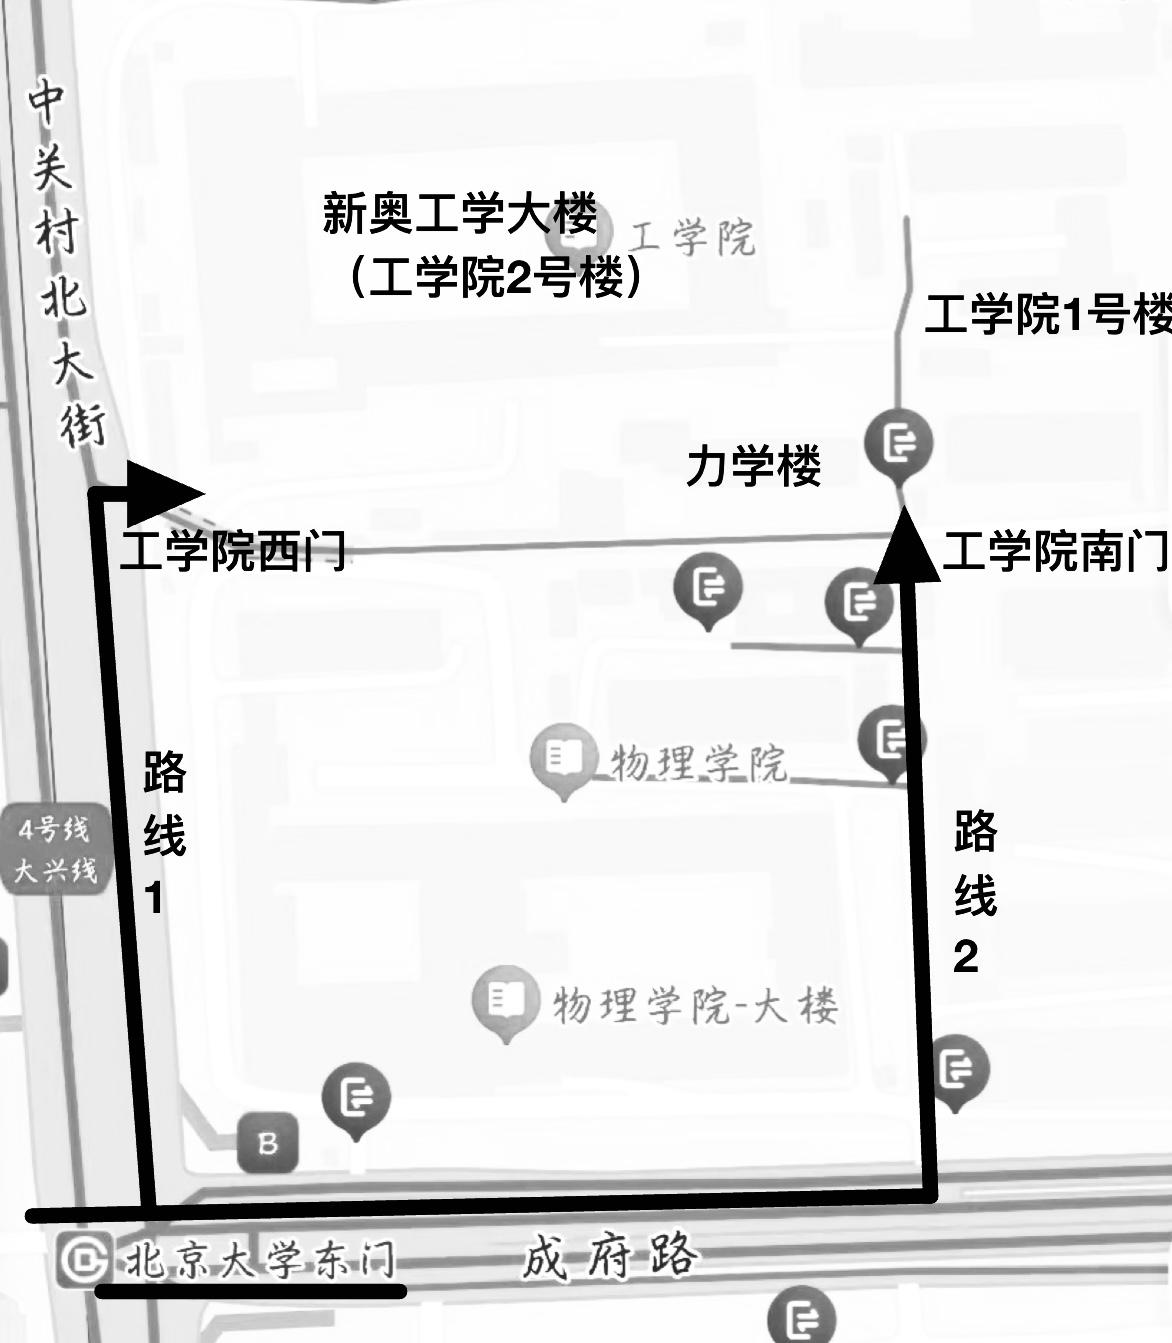
\includegraphics[width=0.5\linewidth]{assets/6.1工学大院地形.jpeg}
	\renewcommand{\figurename}{图}
	\caption{工学院主要建筑分布及通勤路径}
	\label{fig:enter-label}
\end{figure}

教务办公室、学生工作办公室均已搬入新奥工学大楼，分别位于2005室和2012室。负责其他事务的办公室位置也可进入工学院官网——办公服务——工学院办公室一栏查看。

\vspace{10pt}

需要提醒大家的是，老师们的办公室并非一定在新奥工学大楼内。故建议大家在与老师面谈前确认老师办公室所在地点。

\vspace{10pt}

工学院的三栋主要建筑内都有会议室。大多数情况下，学院内的大规模会议在这些地方举行：力学楼434，1号楼210，新奥工学大楼3004。

\vspace{10pt}

此外，燕南园60号也是工学院部分部门的办公地点，院子东北角立有写着“北京大学工学院”字样的石碑，是工学院新生打卡圣地。同学们通勤穿过燕南园时经常能路过60号院。

\vspace{10pt}

环境科学大楼（简称环境大楼）是北京大学环境科学与工程学院的教学科研大楼，大楼坐落于北京大学主校园的东北部成府园内，东临中关村北大街，毗邻微纳电子大厦、廖凯原楼（政府管理学院大楼）。

\vspace{10pt}

大楼集教学、科研、办公及学术交流于一体，包含地上五层，地下三层，房间编号是从西南角开始，逆时针方向连续编号。教学办公室（环境大楼104）与学生工作办公室（环境大楼212）位于大楼的一、二层，其余行政老师的办公室地点及联系方式可在“环境学院官网——师资队伍——行政人员”处进行查询。老师办公室与实验室主要位于大楼的三至五层，可在“师资队伍——在职教师”处查询老师们的办公地点与邮箱。

\vspace{10pt}

大楼负一层主要为会议室（B104、B110、B112、B121、B122、B130，以及一层的101室），会议室在无人使用时开放用作自习室，开放时间为8:00-23:00。

\vspace{10pt}

此外，大楼每层均设置有茶水间，并提供微波炉，有需要的同学可按照操作提示进行使用。

\section{信息渠道}
主动高效地获取、筛选信息，是每一位大学生的必修课。这门课优秀与否，在相当大的程度上决定了大家的学业水平和生活水平——某一门课的复习资料和往年题、诺奖得主的学术讲座、百讲的电影首映礼、校园十佳歌手决赛的门票领取……

\vspace{10pt}

进入大学，中学时代信息主动找上门的模式一去不复返，原地等待老师、学长学姐、同学、室友等他人告知的最终结局就是成为信息孤岛，错失关键大事。笔者曾耳闻某位同学四日未打开自己的校园邮箱，导致错失某关键奖项的申请——他本可以十拿九稳。此事虽是个例，却也足以说明主动掌握信息的重要性\footnote{以及每日检查邮箱的重要性！}。因此，我们建议大家充分利用各类渠道，尽快建立信息网络，将信息主动权掌握在自己手中。

\vspace{10pt}

在此，我们列出最为常用的各类渠道，以便大家日常使用，提高主动搜集、整理信息的能力。

\subsection{网站}

1. 北京大学信息门户\quad portal.pku.edu.cn

包含北大日常生活所需80\%的工具和信息，如校园卡（含充值、挂失等）、校园邮箱、校历、课表查询、成绩查询、体育场馆预约、访客预约、空闲教室查询、畅行清华等。同时有手机端APP，推荐大家安装，功能几乎相同，虽然界面适配仍待改进。

\vspace{10pt}

2. 北大树洞\quad treehole.pku.edu.cn

专属于北大人的匿名聊天平台。可查询数量极为庞大、内容极为丰富的民间信息，包括但不限于学习资料、课程评测、院系/专业体验、导师推荐、活动经验、生活技能、恋爱教程、美食攻略、旅游指南、跳蚤市场等。一言以蔽之：无数精彩内容等待大家探索！

需要注意的是，树洞上也有许多没有多少价值的内容，且发帖者（洞主）的立场和偏见、信息真假等均需自行辨别。此外，即使是匿名平台，也请大家务必注意遵守底线思维，不可发表违背公序良俗或法律法规的言论。

\vspace{10pt}

3. 北京大学教务部\quad dean.pku.edu.cn

包含北大有关课程、考试的种种信息，例如培养方案、选课退课、双专业/辅修、本科生科研等。任何学业、课程、政策等有关问题均可在该网站尝试搜索。

\vspace{10pt}

4. 北京大学选课网\quad elective.pku.edu.cn

顾名思义，选课期间最为重要的网站之一。选课网基本操作详见本手册2.3。

\vspace{10pt}

5. 北京大学教学网\quad course.pku.edu.cn

包含已选课程的相关信息，例如教师通知、课程回放、大纲、教案、作业、成绩\footnote{据笔者经验，只有少数课程成绩会在教学网上记录，大多数课程的成绩只出现在树洞上}等。

鉴于极具年代感的网页设计，笔者不得不向大家推荐一份专门美化教学网页面的插件：\\https://github.com/zhuozhiyongde/PKU-Art。具体下载、安装、使用方式，详见GitHub页面的详细说明。注意，笔者仅作推荐，不承担因使用该插件造成的任何损失。

\vspace{10pt}

6. 北京大学学生邮箱\quad mail.stu.pku.edu.cn 

稍正式沟通、交流的常用平台之一。学校或院系通知、活动项目、志愿者招募、师生交流等均会用到学生邮箱。需要注意的是，部分有价值的邮件可能会因判断机制被归入垃圾邮件，而不会出现在收件箱中。故在常规的收件箱之外，垃圾邮件亦需定期检查。

\vspace{10pt}

此处为大家透露一个小彩蛋：学校信息中心会不定期组织钓鱼邮件攻防演练，发送各类与大家学习、生活、兴趣等密切相关的模拟钓鱼邮件，“勾引”大家填写自己的学号和密码，随后跳转至“老师/同学，您已中招”的界面。笔者曾经历校园卡充值满减、端午节免费送粽子、新生情况有奖调查、免费试用Sora大模型等“勾引主题”。在提升诈骗防范能力的同时，笔者也不得不感慨信息中心花样真多（$\times$）。但是，认真地！大家作为新生，一定要提高防范意识，谨防网络诈骗！

\vspace{10pt}

7. 北京大学工学院\quad coe.pku.edu.cn

包含与工学院相关的信息、文件、新闻等，可查询各功能处室办公地址、奖学金评选通知、各专业培养方案、各系所教师队伍、各老师的研究方向和联系方式等。建议大家空闲时了解了解各位老师的研究方向，感兴趣的可以和老师多多交流，甚至可以进入老师的课题组，开启科研体验。早一些接触科研训练对本科生而言，总不是什么坏事。

\vspace{10pt}

8.北京大学环境学院\quad cese.pku.edu.cn

包含环境学院概况、教师信息、招生招聘信息，以及学院重大新闻等。

\vspace{10pt}

9. 北京大学信息中心\quad its.pku.edu.cn

校园网连接设备管理、网费充值、常见问题解决方案，正版软件（如Adobe系列、Microsoft Office、MATLAB等），邮箱使用指南等校园内一切有关“信息”的内容。

\vspace{10pt}

10.北大研招网\quad admission.pku.edu.cn

查询北大研究生招生、录取信息。

\vspace{10pt}

11.北大图书馆\quad www.lib.pku.edu.cn

提供北大图书馆图书借阅、研讨空间预约、活动/展览/讲座等信息。
	
\newpage

\subsection{公众号与小程序}

\[
\begin{matrix}
	\text{北京大学} & \text{公众号} & \text{正身自然不必多说}\\
	\text{工映青春} & \text{公众号} & \text{工学院学生活动信息平台，会发布一些重要通知}\\
	\text{北大体育} & \text{公众号} & \text{85km跑、五四跑、新生杯、北大杯等体育赛事通知}\\
	\text{PKU体委} & \text{公众号} & \text{85km跑相关通知，周二、周四夜奔点歌渠道}\\
	\text{赛艇先生} & \text{公众号} & \text{考试复习资料、往年题}\\
	\text{北大团委} & \text{公众号} & \text{团委活动通知，如中秋晚会、五四诗会等}\\
	\text{北京大学学生会} & \text{公众号} & \text{学生会活动通知，如十佳歌手、十佳主持人等}\\
	\text{P大CoE教务} & \text{公众号} & \text{工院教务公众号，发布学业、课程相关重要通知}\\
	\text{北京大学百周年纪念讲堂} & \text{公众号} & \text{电影、演出等信息}\\
	\text{北大与世界} & \text{公众号} & \text{对外交流项目相关信息}\\
	\text{北大就业} & \text{公众号} & \text{就业指导相关信息}\\
	\text{北大工学} & \text{公众号} & \text{工学院新闻、学术、科研等通知}\\
	\text{北大环院} & \text{公众号} & \text{环境学院最新动态与新闻}\\
	\text{北大环院人} & \text{公众号} & \text{团委、学生会、研会信息发布、活动宣传与风采展示平台}\\
	\text{北京大学学生发展支持} & \text{公众号} & \text{学业辅导、生涯规划等方面的支持}\\
	\text{北大餐饮中心官方资讯} & \text{公众号} & \text{食堂、菜品、特色美食信息}\\
	\text{北京大学图书馆} & \text{小程序} & \text{馆藏内容检索、云打印服务等}\\
	\text{北大空间} & \text{小程序} & \text{预约空闲教室用于自习等}\\
	\text{志愿北京} & \text{小程序} & \text{查看志愿服务学时}\\
	\text{北大文创} & \text{小程序} & \text{文创产品的线上购买、邮寄等}\\
	\text{动力中心收费服务号} & \text{小程序} & \text{查询宿舍用电购电情况，及时充值缴费购电}\\
	\text{燕园学子微助手} & \text{小程序} & \text{北京大学学生工作部发布校园活动宣传推送}\\
\end{matrix}
\]

\subsection{软件}

1. 北京大学APP

与北大门户网站功能相似。

\vspace{10pt}

2. bilibili

无数宝藏课程的荟萃地，同时也是娱乐的天堂。

\vspace{10pt}

3. MATLAB

工学院必备，但大一用处不算大，可提前学习掌握。

\vspace{10pt}

4. 各类IDE软件

IDE（Integrated Development Environment），集成开发环境。用于编写代码，

如Visual Studio Code、PyCharm、Spider、Dev C++等，具体可咨询计算机课程老师或助教，自行比较择优即可。

\vspace{10pt}

5. 手写笔记软件

Goodnotes、Notability、Notein一笔记等，用于手写笔记、绘图等。笔者自觉好用的（例如上述三者）均需付费\footnote{提醒：切勿相信各类低价Goodnotes/Notability账号信息，笔者曾购买所谓永久账号，使用了三周便被封禁（悲）。擦亮双眼，不贪小便宜！}。注意：定期备份！毕竟谁也不想看到软件bug让辛辛苦苦写了一学期的数分笔记在期末周灰飞烟灭。

\subsection{校内联系电话}

\textbf{·保卫部：62755110}

\textbf{·燕园派出所：62751331}

生病、受伤等无法自主行动时，可拨打保卫部电话，前往校医院。

\vspace{10pt}

\textbf{·心理咨询中心：62760852}

\textbf{·24小时心理援助热线：62760521}

情绪没有对错，困难不必独行。笔者真诚地希望你在逐梦的路上，也能照顾好自己的心灵。

\vspace{10pt}

\textbf{·校医院：62759011}

\textbf{·校医院24小时急诊电话：62751919}

\vspace{10pt}

\textbf{·勺园酒店：62752218，62757361，62752200}

\textbf{·中关新园：62755236}

若大家有同学、亲友到访且需住宿，可通过上述电话联系酒店预定房间。持学生卡预定可享受优惠。


\backmatter

\chapter*{后记}
后记是笔者的一点碎碎念。我们非常感谢各位读者能够有耐心阅读到这里。

\vspace{10pt}

本手册从2023年9月22日学术部例会上名为“Engineering DIY”的构想，到2024年8月的初具雏形，再到2025年7月、2026年7月的逐步修订，学术实践部一直致力于打破信息壁垒，希望能够对各位初入工院的读者有所帮助。在此，诚挚感谢所有对本手册的编写和修订作出贡献的老师和同学们。

\vspace{10pt}

%人名
\textbf{以下是参与《北京大学工学院新生生存手册》制作的全体人员名单：}

\textbf{主编：赵丹枫\hspace{6pt}倪\hspace{11pt}昊\hspace{6pt}武昱达}

\textbf{第二版主编：古冠群\hspace{6pt}郑雅文\hspace{6pt}郭濠源}

\textbf{第三版主编：王晨锦\hspace{6pt}田\hspace{11pt}特\hspace{6pt}孙兆梓骞}

\textbf{封面美工：周文硕\hspace{6pt}田浩远}

\textbf{文字作者：}

\textbf{2020级本科\hspace{20pt}王一诺\hspace{6pt}瞿朱毅}

\textbf{2021级本科\hspace{20pt}刘家豪\hspace{6pt}李一川\hspace{6pt}吴秉宪\hspace{6pt}杨铮昊\hspace{6pt}钱骏飞\hspace{6pt}谢谊锋}

\textbf{2022级本科\hspace{20pt}王喆楷\hspace{6pt}付\hspace{11pt}杨\hspace{6pt}李昆泰\hspace{6pt}范文琳\hspace{6pt}赵丹枫\hspace{6pt}郭\hspace{11pt}祺}

\textbf{\hspace{82pt}秦\hspace{11pt}晟\hspace{6pt}曹林博\hspace{6pt}曾帅鹏程}

\textbf{2023级本科\hspace{20pt}李宗远\hspace{6pt}武昱达\hspace{6pt}倪\hspace{11pt}昊}

\textbf{2024级本科\hspace{20pt}古冠群\hspace{6pt}郑雅文\hspace{6pt}郭濠源}

\textbf{2025级本科\hspace{20pt}常宇宁\hspace{6pt}王晨锦\hspace{6pt}田\hspace{11pt}特\hspace{6pt}孙兆梓骞}

\textbf{特别鸣谢：刘牧时\hspace{6pt}陈\hspace{11pt}正\hspace{6pt}尹子馨\hspace{6pt}张瑞石\hspace{6pt}刘\hspace{11pt}涵\hspace{6pt}朱若珊\hspace{6pt}苑湘崎}

\textbf{监制：陈泽宇\hspace{6pt}何沐祺}

\textbf{以及几位希望保持匿名的同学，再次感谢所有老师们和同学们的付出！}

\vspace{10pt}

由于编者水平所限，手册还存在许多失误和疏漏亟待完善，敬请读者指正。任何关于《北京大学工学院新生生存手册》的纠错和建议，欢迎通过以下方式和我们联系。提前感谢各位对本手册做出的贡献！

\begin{figure}[htbp]
	\centering
	
\includegraphics[width=0.2\linewidth]{assets/后记二维码.png}
\end{figure}

人生是旷野，不是轨道。北大是沃土，不是硬岩。笔者衷心希望各位读者能够灵活应用本手册提供的信息，为自己创造出似锦前程，创造出不设限的人生。

\begin{flushright}
	2026年8月
\end{flushright}



\chapter*{结语}
雅思贝尔斯讲：“教育是一棵树摇动另一棵树，一朵云推动另一朵云，一个灵魂唤醒另一个灵魂。”笔者自知身为“先行者”，决不能耳提面命，不能高高在上，不能不容置疑。诚望能将自己的经验、自己走过的道路汇编成册，抛砖引玉式地为读者提供参考，让读者更快更好地“上手”大学生活。

\vspace{10pt}

洋洋洒洒写到结尾，笔者深知前文中仍有片面的、主观的认识，若对读者造成困扰，还望见谅。

\vspace{10pt}

人生是旷野，不是轨道。我们真诚地祝愿读者不囿于一隅，能够在这片旷野里恣意奔跑，在燕园中纵情挥洒青春年华。

\vspace{10pt}

\begin{flushright}
	武昱达
	
	2024年8月
\end{flushright}
\fullbleedpage{assets/封底.jpg}


\end{document}
